\documentclass[
  12pt      
  ,letterpaper
  ,center
  ,noupper
  ]{uconnthesis}
\ThesisLineSpacing{2}
\usepackage{graphicx}  % needed for figures
\usepackage{subeqnarray}
\usepackage{cases}
\usepackage{bm}        % for math
\usepackage{amssymb}   % for math
\usepackage{epstopdf}

\newcommand{\adag}{\ensuremath{a^{\dagger}}}
\newcommand{\bdag}{\ensuremath{b^{\dagger}}}
\newcommand{\cdag}{\ensuremath{c^{\dagger}}}
\newcommand{\ddagg}{\ensuremath{d^{\dagger}}}
\newcommand{\ket}[1]{\ensuremath{\left| #1 \right\rangle}}
\newcommand{\bra}[1]{\ensuremath{\left\langle #1 \right|}}
\newcommand{\braket}[2]{\ensuremath{\left\langle #1 \right|\left. #2\right\rangle}}
\newcommand{\mele}[3]{\ensuremath{\left\langle #1 \right|#2\left| #3\right\rangle}}
\newcommand{\dyad}[2]{{\ket{#1}\!\!\bra{#2}}}
\newcommand{\norm}[1]{\ensuremath{\left\| #1 \right\|}}
\newcommand{\abs}[1]{\ensuremath{\left| #1 \right|}}
\newcommand{\To}{\ensuremath{\rightarrow}}
\newcommand{\from}{\ensuremath{\leftarrow}}
\newcommand{\funE}{\ensuremath{\mathcal{E}}}
\newcommand{\beq}{\begin{equation}}
\newcommand{\eeq}{\end{equation}}
\newcommand{\bea}{\begin{eqnarray}}
\newcommand{\eea}{\end{eqnarray}}
\newcommand{\mbf}[1]{\ensuremath{\mathbf{#1}}}
\newcommand{\eq}[1]{{(\ref{#1})}}
\newcommand{\commentout}[1]{{}}
\newcommand{\idx}{{l}}
\newcommand{\half}{{\hbox{$\frac{1}{2}$}}}
\newcommand{\Kappa}{{\cal K}}
\newcommand{\bE}{{\bf E}}
\newcommand{\br}{{\bf r}}
\newcommand{\cbE}{\boldsymbol{\mathbf{\cal E}}}
\newcommand{\dip}{{\cal D}}
\newcommand{\G}{{\sf G}}
\newcommand{\bd}{{\bf d}}
\newcommand{\red}[1]{\textcolor{red}{#1}}
\newcommand{\blue}[1]{\textcolor{blue}{#1}}
\newcommand{\ja}[1]{\red{#1}}
\newcommand{\js}[1]{\textcolor{blue}{\textst{#1}}}

\begin{document}
\bibliographystyle{prsty}

\abstract{
At high density, dipole-dipole interactions between the atoms may have a major impact on light propagation in a dense gas. We have developed a classical-electrodynamics simulation to study the cooperative response of a near-resonant gas to light. We take into account the motion of the radiators using classical trajectories, including collisions with the walls of the container and atom-atom collisions, and describe the transition from homogeneously broadening to inhomogeneously broadened phenomenology.
}

\title{Cooperative Effects in the Optical Response of Dense Atomic Gases}
\author{Yi Li}
\authorspreviousdegreelong{
  B.S., University of Science and Technology of China, Hefei, China, 2007 \\
  M.S., University of Connecticut, 2010
  }
\authorspreviousdegreeshort{M.S.}

\MajorAdvisor{Juha Javanainen}
\AssociateAdvisorA{Robin C\^ot\'e}
\AssociateAdvisorB{William Stwalley}

\dedication{
To ...
  }

\acknowledgements{
Thank you.
  }

\maketitle
\frontmatter
\tableofcontents
\listoffigures
\listoftables

\mainmatter

\chapter{Introduction}

\section{Light scattering and cooperative effects}

Light scattering is the primary mechanism of physical observation. The state of the light field would carry a great deal of information about the object with which the light had just interacted. A simple example is that one can tell the shape and color of an object by receiving the light scattered off its surface.

%Along with the exploration of the essence of light itself, the application of light as an indispensable tool to study the property of matter has achieved tremendous success since the dawn of modern science. 
 
With the development of physics, the model of light kept getting more comprehensive. Beyond the simple ray model in geometrical optics, wave properties of light were introduced in the scope of physical optics. Later, within the framework of classical electrodynamics, light scattering became satisfactorily explainable. Examples include Rayleigh and Mie scattering. Both mechanisms are based on discrete radiators in a liquid or gaseous medium, where each particle (e.g. an atom or a molecule) deflects the incoming light independently.

Assuming the light wavelength is $\lambda$ and the dimension of a particle is $D$, in the small particle regime ($D\ll\lambda$), Rayleigh scattering would be observed~\cite{Lilienfeld:04}. As an elastic scattering process, each particle is treated as a classical dipolar radiator that oscillates at the same frequency as the incoming electric field and then re-radiates the field outward. In Rayleigh scattering, the relative strength of the scattered light is proportional to $\lambda^{-4}$. This is the reason for the blue sky for the shorter wavelength is scattered much stronger than the longer wavelengths.

When the size of the scattering particles is comparable to the wavelength ($D\sim\lambda$), the Rayleigh model would break down. One can instead solve the Maxwell equations that describe a plane wave scattered by a homogenous sphere with an infinite series of spherical harmonics. This solution is Mie scattering~\cite{1908AnP...330..377M}. 

There are some remarkable features of Mie scattering that make it different from Rayleigh model. For example, the strength of the scattered light is greater in the forward direction than in the backward direction; the larger the particle, the more of light is scattered in the forward direction. 

We mention Rayleigh and Mie scattering for they have features similar to the light scattering process in dense gases that we study in the dissertation.

%The optical property of a medium hinges on the nature of light-matter interactions that take place inside it.

In many cases, light scattering, as an important aspect of optical response to light, is responsible for the optical property of a medium. For example, the light attenuation inside a medium of independent radiators is partially due to the scattering of light in directions other than the one of the incident light beam. For a linear and isotropic medium, the Beer-Lambert law relates the relative intensity of the transmitted light to the optical thickness $\mathcal{D}$ of the sample:
\bea
I_{out}=I_{in}\,e^{-\mathcal{D}}.
\label{BEER'S_LAW}
\eea
This relation is one of the theoretical bases of absorption imaging, a commonly used technique to access information of the sample in cold atom experiments. The law tends to break down in a very dense sample, where the atoms or molecules are so close to each other that the interaction between the particles will change their internal states, and thus will change the attenuation. 

%Another possibility that this law fails could happen when the light is quite intense, the nonlinear optical processes will then alter the bulk property of the sample.


%(cooperative effects; time domain: superradiance; frequency domain: CLS)~\cite{PhysRevLett.112.113603}

%(mean-field theory; continuous medium; independent radiators; interacting radiators.)

%(light-matter interaction: from simple to complex: classical scattering, attenuation, fluorescence, polarization of a medium, ensemble-light interfaces)

%The Beer-Lambert law does not distinguish microscopic mechanisms of the light attenuation, such as absorption and scattering by atoms in the sample. Moreover, it also neglects all the other attributes of the light except the intensity. 

%\section{The role of light in modern physics}

In the era of modern physics, the role of light scattering is even more important. Of course, light is still a natural and feasible way of probing the state of the material with which it interacts. For example, at the time of the first realizations of Bose-Einstein condensates~\cite{Anderson14071995,PhysRevLett.75.3969}, the properties of light scattering from BECs were widely discussed~\cite{PhysRevA.43.6444,PhysRevA.51.3896,PhysRevA.52.3033,PhysRevLett.71.1339}  and a number of proposals for employing light scattering to detect BECs were raised. Characteristic details in the line shape for light scattered from BECs were predicted for different configurations~\cite{PhysRevLett.72.2375,PhysRevA.50.R3565,PhysRevLett.75.1927,PhysRevLett.76.1774,PhysRevA.54.R2543}. Though much trickier than one might wish, it is in principle possible to verity the existence of a Bose-Einstein condensate by spectral measurements of the scattered radiation from an atomic sample. Another example of theoretical proposal is probing quantum statistics of atoms in an optical lattice by light scattering~\cite{PhysRevA.76.053618}. In practice, for instance, an experiment that used light scattering to determine the relative phase of two Bose-Einstein condensates has been carried out~\cite{Saba25032005}.

Furthermore, in the context of quantum measurement theory, light scattering is likely to be a common probe for nondestructive measurements~\cite{RevModPhys.68.1} , continuous observation, and feedback control. For example, a nondestructive measurement to probe the quantum state of a 1D Bose gas using off-resonant light scattering was proposed\cite{PhysRevLett.107.270403}. Another example is monitoring continuously and non-destructively the number of atoms in a Bose-Einstein condensate by light scattering as the atoms oscillate back and forth between two sides of a double-well trap\cite{NJP.JJ}.

From a even broader perspective, the understanding of light-matter interactions, including light scattering, is critical for the work on controlling quantum systems, which in turn opens the way for practical techniques such as quantum computer and quantum communication. One approach to handle the light-matter interaction is cavity quantum electrodynamics (cavity QED)~\cite{0034-4885-69-5-R02}. In general, a week coupling between the cavity field and the atoms leads to modifications of the internal state of the atoms. In the strong coupling case, atoms and photons are entangled, this being the basis of a lot of interesting applications. A lot of fascinating experiments have been preformed such as photon blockade~\cite{photon_blockade}.

Another way to deal with light-matter interaction is via atomic ensemble-light interface. To be specific,  optically thick free space ensembles can be efficiently interfaced with quantum optical fields~\cite{RevModPhys.82.1041}. In recent years, this approach has become a very active area of research. Comparing to ensembles of independent or weakly correlated atoms, in an atomic ensemble with a large optical depth, the strong correlation between atoms dramatically alters the way the light and atoms interacts. Various mechanisms including quantum feedback control and electromagnetically induced transparency have also been studied extensively on the basis of the quantum interface between atomic ensembles and light. Finding a thorough understanding of the optical response of a atomic ensemble to light is a challenging task. For instance, as a classical analogy, light scattering in a optically dense medium becomes a collective behavior of the whole system, which is much trickier to handle in mathematics.

Experimentally, the cooperative effects in light scattering have been studied intensively in recent decades.  Superradiant Rayleigh scattering from a Bose-Einstein condensate was studied\cite{Inouye23071999,PhysRevLett.83.5202,PhysRevA.62.063615} and cooperative Mie scattering from an ultracold atomic cloud was also observed\cite{PhysRevA.82.011404}. Moreover, recent experiments demonstrated that the density fluctuations in the atomic cloud tend to suppress cooperativity\cite{PhysRevLett.104.183602}, and that the cooperativity generates a shift of the optical transition frequency that depends on the density and geometry of the atomic sample\cite{PhysRevLett.108.173601}. The cooperative effects also lead to the phenomenon that the radiation pressure of a laser beam would be modified by the scattered photons\cite{Eur.Phys.J.D.58.1}.

The importance of light-matter interaction calls for more insights into cooperative effects in the medium which the light passes through. However, analysis of cooperative response of a dense medium is a challenge because of the combination of the strong short-range divergence $(1/r^3)$ and the long range $(1/r, $ for radiating atoms$)$ of the dipole-dipole interactions. The literature is replete with approximations\cite{FRIEDBERG1973101}. In this dissertation we promote an alternative approach, numerical simulations of classical light propagating in a medium of classical induced dipoles. Starting from quantum field theory for both atoms and light, it has been shown\cite{PhysRevA.55.513} that such an approach is valid basically when photon recoil and saturation of the atoms may be neglected. We develop software objects in C++ to carry out classical light propagation studies in an (in principle) arbitrary collection of classical dipoles, and use them to understand the emergence of the cooperative effects in common geometries. Our classical simulations of inhomogeneously broadened samples improved and perfected traditional optical theory on some well-known cooperative effects. Moreover, simulations with moving atoms verifies existing theoretical predictions and reveals new features in spectroscopic observations that can be categorized as cooperative.


\section{Outline}

In Chapter 2, the theoretical basis of the research is reviewed. As a fundamental content of quantum optics, the semi-classical theory of the interaction between a two-level atom and a classical light field is briefly restated. The polarizability of an atom as a damped two-level system is particularly emphasized for this is related to two primary aspects of cooperative effects: absorption and resonance shift. Additionally, we also introduce the local-field correction and Clausius-Mossotti equation in this chapter, for they are critical in analyzing cooperative effects that we will see later in the dissertation.

Chapter 3 qualitatively describes two typical types of cooperative effects in a system of strongly interacting dipoles. While observing the fluorescence from a dense sample, the emitted field intensity is much stronger and the duration of the pulse is much shorter than that from a system of independent atoms. We recap Dicke's pioneering work on the superradiance model in this chapter. On the other hand, in the frequency domain, besides the generic Lorentz-Lorenz shift brought by the local-field correction in the absorption spectrum, another type of shift called collective Lamb shift can be observed in a dense sample for atoms are correlated with the virtual photons of the QED vacuum. We emphasize superradiance and CLS here for they are phenomena that repeatedly come up in our research. In the last section of this chapter, the exact definition of cooperativity is discussed before we initialize further calculations and simulations.

As the primary technique in our research, classical simulation is introduced in the beginning of Chapter 4. After the discussion about the validity and scope of application of our simulation, we firstly solve the problem of light scattering from a single atom and a two-atom system. Then detailed calculations are carried out on a hypothetical cloud of independent radiators whose spacial distribution is Gaussian.  When dipole-dipole interaction is added to this Gaussian cloud, we find from simulation that the cooperative effect in emission intensity shows up at an unexpectedly low density. The simulation of the Gaussian cloud is followed by a more realistic simulation on a dense gas in a circular disk container. The most important technique we employ in this simulation is the addition of an artificial inhomogeneous broadening to the sample. We find that such a broadening in the system of discrete radiators leads to close agreement with the collective Lamb shift predicted by the traditional mean-field theory.

In Chapter 5, an important feature is added into the simulation, that is the atomic motion. When atom-atom and atom-wall collisions as well as free flight in-between are taken into account, the model becomes more comprehensive and hence able to display more intriguing phenomena. Both the direct calculation on a single atom and the simulation of indecent atoms generate a narrowed peak of resonance in the absorption spectrum. This is a clear signature of Dicke narrowing due to atomic collisions. Again, things are different when atoms are strongly correlated. When we introduce dipole-dipole interactions between atoms, the thickness-dependent attribute of the collective Lamb shift is unaltered. However, the width of the resonance peak in this case becomes another signature of cooperativity. The transition from a clearly Dicke narrowed peak in a dilute gas to a greatly broadened peak in a optically dense sample is observed in simulation.

Finally, we summarize our work in Chapter 6 and prospect the work direction of the aftertime.


%Apparently, the success of classical scattering theories such as Rayleigh and Mie scattering results from the fact that the model with classical dipoles is much more realistic than the continuous-medium model. 

%However, it doesn't end here. The fundamental principles that rule the real world is quantum, not classical, including both sides of the light-matter interactions. Quite a lot of optical phenomena could only be interpreted by quantum theories. A prime example is the spontaneous emission of atoms.

%A well known semi-classical description of spontaneous transitions is given by the Einstein A and B coefficients. In this framework, the atom is quantized but the electromagnetic field is not. 

%In an ordinary fluorescence experiment of two-level atoms, assume that the sample has $N(0)$ atoms initially prepared in the upper level, then the number of excited atoms at time $t$ is given by
%\bea
%N(t)=N(0)e^{-At}=N(0)e^{-\Gamma t}=N(0)e^{-t/\tau},
%\eea
%where the Einstein A coefficient is just the spontaneous decay rate $\Gamma$, which in turn equals to the reciprocal of the lifetime $\tau$.

%The fundamental mechanism of spontaneous transition can only be explained by a quantized electromagnetic field. In quantum electrodynamics, the spontaneous transition in free space is a consequence of the interaction between the atom and the QED vacuum. In the dipole approximation, the rate of spontaneous emission $\Gamma$ is given by
%\bea
%\Gamma=\frac{k^3d^2}{3\pi\hbar\epsilon_0}.
%\eea
%Given a sample composed of independent atoms, due to the infinite number of degrees of freedom of the electromagnetic field, the radiation pattern of the spontaneous emission would be essentially isotropic.

%In summary, if the constituent particles are treated as independent radiators, i.e., the sample is sufficiently dilute so the interaction between particles is neglected, the eventually observable electromagnetic field from a sample can be predicted as a simple superposition of the post-interaction fields (photons) from all the particles in the sample. The interacting field can be vacuum or not.







\chapter{Semiclassical Theory of Interaction between Two-level Atom and Classical Light}

\section{Electrodynamics of a polarizable medium: Local-fleld correction and Clausius-Mossotti equation}

In a dense liquid or gaseous medium, the field on an individual atom will be influenced by the polarization of the atoms in its close neighborhood. %In other words, if the medium is uniformly polarized, an atom will feel a local field that differs from the field in the medium.

Conventionally, a mean-field theory (MFT) is used to study the local field. An arbitrary atom in such a medium is surrounded by the other atoms~\cite{feynman}. The field on the site of this atom $\cbE_{loc}$ can be approximated by the field in a small spherical hole that centered at the position of the atom. Imagine that this spherical hole is made by "scooping out" a sphere of the polarized material, assume $\cbE$ is the average field in the medium and $\cbE_{sphere}$ is the field inside the scooped out sphere, because of the superposition, we have
\bea
\cbE=\cbE_{loc}+\cbE_{sphere}.
\label{E_MEAN}
\eea

Note that the sphere is also uniformly polarized, therefore the field inside the sphere is uniform, the value is given by
\bea
\cbE_{sphere}=-\frac{\mathbf{\cal{P}}}{3\epsilon_0},
\label{E_SPHERE}
\eea
where  $\mathcal{P}$ is the polarization.

Combining Eq.~\eq{E_MEAN} and Eq.~\eq{E_SPHERE}, we obtain the expression of the local field at the position of an atom in a uniformly polarized medium as
\bea
\cbE_{loc}=\cbE+\frac{\mathbf{\cal{P}}}{3\epsilon_0},
\label{LOCAL_FIELD}
\eea
The correction term $\frac{\mathbf{\cal{P}}}{3\epsilon_0}$  is referred to as the local-field correction. We will encounter with this correction repeatedly in later chapters where we will discuss the interpretation of this correction by means other than the conventional mean-field theory.

For now, we can take one more step forward. Assume $\alpha$ is the polarizability of each individual atom and there are $N$ identical atoms in the medium, since the real field felt by each atom is $\cbE_{loc}$ given by Eq.~\eq{LOCAL_FIELD}, we have
\bea
\mathbf{\cal{P}}=4\pi\epsilon_0N\alpha\cbE_{loc}=4\pi\epsilon_0N\alpha\left(\cbE+\frac{\mathbf{\cal{P}}}{3\epsilon_0}\right).
\label{POLARIZATION}
\eea
Remembering that the susceptibility $\chi$ is just $\mathbf{\cal{P}}/\epsilon_0\cbE$, from Eq.~\eq{POLARIZATION} we can readily derive the Clausius-Mossotti equation (Lorentz-Lorenz law) as:
\bea
\chi=\frac{4\pi N\alpha}{1-\frac{4}{3}\pi N\alpha}.
\label{LLLAW}
\eea
This equation is a bridge between the bulk property of a sample ($\chi$) and the response of individual atoms to the external light field ($\alpha$). The exact form of $\alpha$ is determined by the internal structure of the atom and the nature of the light. We will see specific examples in later chapters too.


\section{Interaction of a two-level atom with a classical field}

Now let us get back to the problem of the response of a quantum two-level atom to a classical electric field, which is one of the simplest nontrivial models involving the atom-field interaction\cite{quantum_optics}. As a semiclassical model, it allows us to extract essential features of atom-field interactions and provides rather satisfactory explanations to many optical phenomena. As a matter of fact, most of our research is primarily based on this model. Therefore, it is worthwhile to recap some core concepts here.

\subsection{Einstein $A$ and $B$ coefficients}
Einstein used $A$ and $B$ coefficients to formulate a purely phenomenological theory of  absorption and emission of light by an atom~\cite{quantum_optics,1982AmJPh..50..982H}.

We assume $N$ identical two-level atoms with a lower bound-state energy level $E_1$ and a higher level $E_2$. The photon emitted or absorbed by the atom has an energy equal to the difference between two levels, i.e., $\hbar\omega_0=E_2-E_1$.

Three processes exist simultaneously in the atom-field interaction: spontaneous emission, stimulated emission and absorption. Accordingly, there are three phenomenological constants $A_{21}$, $B_{21}$ and $B_{12}$.

We also assume the average energy density of the electromagnetic field is $U(\omega)$, the populations of the lower and upper levels are $N_1$ and $N_2$, thus $N_1+N_2=N$, then we can write a rate equation as
\bea
\frac{dN_1}{dt}=-\frac{dN_2}{dt}=A_{21}N_2+B_{21}U(\omega)N_2-B_{12}U(\omega)N_1.
\label{AB_RATE}
\eea
Apparently, $A_{21}$, $B_{21}U(\omega)$ and $B_{12}U(\omega)$ represent the probabilities per unit time for the atom to undergo spontaneous decay, stimulated emission and absorption, respectively. Starting from Eq.~\eq{AB_RATE}, given a certain energy distribution of the field, Eq.~\eq{AB_RATE} is solvable in some cases.

For example, if we have an external light beam incident on atoms, which has a constant energy density such that $U(\omega)\equiv U$, both the lower and upper level are non-degenerate so $B_{21}=B_{12}=B$. We also write $A_{21}=A$, the solution for Eq.~\eq{AB_RATE} is:
\bea
N_1(t)=\left(N^0_1-\frac{N(A+BU)}{A+2BU}\right)\exp\left[-\left(A+2BU\right)t\right]+\frac{N(A+BU)}{A+2BU},
\eea
where $N^0_1$ is the initial population of the lower level.

In the case that $N^0_1$, as $t\to\infty$, we will finally reach the steady state for which we have
\bea
\frac{N_2}{N}=\frac{1}{2+A/BU}.
\eea

Particularly, if we switch off the external field, i.e., $U=0$, Eq.~\eq{AB_RATE} becomes
\bea
\frac{dN_2}{dt}=-N_2A,
\eea
then $N_2(t)=N^0_2\exp(-At)$. This exponential decay of the upper level population with time corresponds to the familiar spontaneous emission. Of course, the ab initio calculation of the $A$ (and $B$ as well) coefficient is not feasible under this framework. A thorough analysis based on quantum field is needed, which will not be covered in this section.

\subsection{Damped two-level system}
Now let us assume that the two-level atom is driven by a classical monochromatic light field
\bea
\bE(\br,t)=\frac{1}{2}\cbE(\br)e^{-i\omega t}+\frac{1}{2}\cbE^*(\br)e^{i\omega t},
\eea
and the two energy eigenstates of the atom is labeled by $\ket{0}$ and $\ket{1}$. The energy difference between the two levels is still $\hbar\omega_0$. Then the atomic Hamiltonian can be written as
\bea
\frac{H_0}{\hbar}=\omega_0\ket{1}\bra{1}.
\eea
In the dipole approximation, the atom-field interaction is
\bea
\frac{H^\prime}{\hbar}=-\hat{\bf{d}}\cdot\bE(t)=-\bE(t)\cdot\left(\bf{d}^*\ket{0}\bra{1}+\bf{d}\ket{1}\bra{0}\right),
\eea
where $\hat{\bf{d}}$ is the atomic dipole operator and $\bf{d}=\bra{1}\hat{\bf{d}}\ket{0}$. Thus we have the Hamiltonian
\bea
\frac{H}{\hbar}=\frac{H_0}{\hbar}+\frac{H^\prime}{\hbar}=\omega_0\ket{1}\bra{1}-\frac{\bE(t)}{\hbar}\cdot\left(\bf{d}^*\ket{0}\bra{1}+\bf{d}\ket{1}\bra{0}\right).
\eea

Next we transform to a rotating frame with a unitary operator
\bea
U=\ket{0}\bra{0}+e^{i\omega t}\ket{1}\bra{1}.
\eea
In order to keep the time dependent Schrodinger equation valid, the transformed Hamiltonian should be defined as
\bea
\tilde{H}&=&i\hbar\frac{dU}{dt}U^{\dagger}+UHU^{\dagger}\nonumber\\
&=&(\omega_0-\omega)\ket{1}\bra{1}\nonumber\\
&&-\frac{1}{2}(\cbE e^{-i\omega t}+\cbE^*e^{i\omega t})\cdot(e^{-i\omega t}\bf{d}^*\ket{0}\bra{1}+e^{i\omega t}\bf{d}\ket{1}\bra{0}).
\eea
In the rotating-wave approximation (RWA), we drop the terms that contain $e^{\pm 2i\omega t}$, define the detuning $\Delta=\omega_0-\omega$ and the Rabi frequency $\Omega=\frac{\bf{d}\cdot\cbE}{\hbar}$, the tranformed Hamiltonian becomes
\bea
\frac{H}{\hbar}=\Delta\ket{1}\bra{1}-\frac{1}{2}(\Omega\ket{1}\bra{0}+\Omega^*\ket{0}\bra{1}).
\label{TRANS_H}
\eea

The Liouvill-von Neumann equation gives the equation of motion of the density matrix as
\bea
\frac{d\rho(t)}{dt}=-i\left[\frac{H}{\hbar},\rho\right].
\eea
In principle, given the Hamiltonian in ~\eq{TRANS_H}, we can solve the equations of motion. However, just as in the Einstein's theory of $A$ and $B$ coefficients, spontaneous emission should be taken into consideration although our model is semi classical. In other words, some relaxation terms due to the coupling between the atom and the quantized electomagnetic field should be added into the system.

First, there is a constant probability per unit time $\Gamma$ for decay from the excited state 1 to the ground state 0, so that we have
\bea
\left.\frac{d}{dt}\right|_R\rho_{11}=-\Gamma\rho_{11},\quad \left.\frac{d}{dt}\right|_R\rho_{00}=\Gamma\rho_{11}.
\eea
We also need to add a relaxation term for the off-diagonal coherences
\bea
\left.\frac{d}{dt}\right|_R\rho_{01}=-\gamma\rho_{01}, \quad \left.\frac{d}{dt}\right|_R\rho_{10}=-\gamma\rho_{10}.
\eea

The density operator is a legitimate density operator if and only if the relaxation terms are of what is known as the Lindblad form,
\bea
\mathcal{L}\rho=\sum_k\left[2L_k\rho L^{\dagger}_k-L^\dagger_kL_k\rho-\rho L^\dagger_kL_k\right],
\eea
where $L_k$ are some system operators. The evolution of the system (atom alone) is described by a master equation of the form
\bea
\dot{\rho}=-\frac{i}{\hbar}[H,\rho]+\cal{L}\rho.
\eea

For the damped two-level system, it is required that $\gamma\geq\Gamma/2$ to ensure the density operator remains positive. If only the spontaneous-emission damping is considered, we can explicitly choose $\gamma=\Gamma/2$. The Lindblad operator is
\bea
L=\sqrt{\gamma}\ket{0}\bra{1}.
\eea

We then have the explicit equations of motion of the elements of the density operator in the matrix form:
\bea
\dot{\rho}_{00}&=&\Gamma\rho_{11}+\frac{1}{2}i(\Omega^*\rho_{10}-\Omega\rho_{01}),\nonumber\\
\dot{\rho}_{11}&=&-\Gamma\rho_{11}-\frac{1}{2}i(\Omega^*\rho_{10}-\Omega\rho_{01}),\nonumber\\
\dot{\rho}_{01}&=&(i\Delta-\gamma)\rho_{01}+\frac{1}{2}i\Omega^*(\rho_{11}-\rho_{00}),\nonumber\\
\dot{\rho}_{10}&=&(-i\Delta-\gamma)\rho_{10}-\frac{1}{2}i\Omega(\rho_{11}-\rho_{00})=(\dot{\rho}_{01})^*.
\label{TWO_LEVEL_EQ}
\eea

Eqs.~\eq{TWO_LEVEL_EQ}, together with the condition of unit trace $\rho_{00}+\rho_{11}=1$, has a steady-state solution as
\bea
\rho_{11}=1-\rho_{00}=\frac{\abs{\Omega}^2/4}{\Delta^2+\gamma^2+\abs{\Omega}^2/2},\quad\rho_{10}=(\rho_{01})^*=\frac{\frac{1}{2}\Omega(i\gamma+\Delta)}{\Delta^2+\gamma^2+\abs{\Omega}^2/2}.
\label{STEADY_STATE}
\eea
$\Gamma\rho_{11}$ stands for the probability per unit time that an atom in an excited state falls down to the ground state. According to the solution of $\rho_{11}$ in ~\eq{STEADY_STATE}, the fluorescence intensity behaves as a function of detuning as a Lorentzian with the maximum at $\Delta=0$ and with the half width at half maximum, HWHM, $\gamma^\prime=\sqrt{\gamma^2+\abs{\Omega}^2/2}$.  In the weak-field approximation, the power broadening from the Rabi frequency becomes negligible, thus the HWHM would be close to the natural width $\gamma$. Again, just as the Einstein $A$ and $B$ coefficient, $\Gamma$  and $\gamma$ are also introduced as phenomenological constants.
\subsection{Polarizability of a two-level atom}
Besides the fluorescence, our strongest interest still lies in the light propagation in a polarizable medium. In the previous section about local-field correction, our discussion ended up with the relation between the susceptibility of the medium $\chi$ and the atomic polarizability $\alpha$. Now let us move on to the expression of $\chi$ for a two-level medium.

Starting from Maxwell's equations in a medium, we have for the electric field an inhomogeneous wave equation
\bea
-\nabla^2\bE+\frac{1}{c^2}\frac{\partial^2\bE}{\partial t^2}=-\frac{1}{\epsilon_0c^2}\frac{\partial^2\bf P}{\partial t^2},
\label{WAVE_EQ}
\eea
where $\bf P$ is the polarization of the medium and $c=1/\sqrt{\mu_0\epsilon_0}$ is the speed of light in vacuum.

For plane waves propagating in the $+z$ direction, the electric field and the polarization can be in the forms
\bea
\bE(\br,t)&=&\frac{1}{2}e^{i(kz-\omega t)}\mathcal E(z,t)\hat{\bf e}+c.c.,\\
\bf P(\br,t)&=&\frac{1}{2}e^{i(kz-\omega t)}\mathcal P(z,t)\hat{\bf e}+c.c.
\eea
The amplitudes $\mathcal E$ and $\mathcal P$ are then supposed to vary slowly in time and space compared with the exponentials. This is called the slowly-varying envelope approximation (SVEA). 

We assume that
\bea
\abs{\frac{\partial\mathcal E}{\partial t}}\ll \omega\abs{\mathcal E}, \quad \abs{\frac{\partial\mathcal E}{\partial z}}\ll k\abs{\mathcal E}, 
\eea
where $k=\omega/c$ and similarly for $\mathcal P$. Neglecting the higher-order derivatives, then Eq.~\eq{WAVE_EQ} is reduced to 
\bea
\frac{\partial \mathcal E}{\partial z}+\frac{1}{c}\frac{\partial \mathcal E}{\partial t}=i\frac{k}{2\epsilon_0}\mathcal P.
\label{BASIC_EQ}
\eea

As an example, consider the case when the electric field amplitude is stationary and the response of the medium is linear:
\bea
\frac{\partial \mathcal E}{\partial t}=0, \quad \mathcal P=\epsilon_0\chi\mathcal E.
\eea
Let us break the susceptibility $\chi$ into real and imaginary parts as $\chi=\chi^\prime+i\chi^{\prime\prime}$, the solution to Eq.~\eq{BASIC_EQ}  is then
\bea
\mathcal E(z)=\mathcal E(0)e^{\frac{1}{2}k(i\chi^\prime-\chi^{\prime\prime})z}.
\eea

It turns out that the intensity of the light will go down along the direction of propagation:
\bea
I(z)\propto\abs{\mathcal E(z)}^2\propto e^{-k\chi^{\prime\prime}z}.
\eea
This is just the familiar Beer-Lambert law.

Next, for the Rabi frequency $\Omega=\bd\cdot\cbE/\hbar$, we assume that $\cbE$ and $\bd$ are proportional to the same real unit vector $\hat {\bf e}$, write
\bea
\bd=d\hat{\bf e}, \quad \cbE=e^{ikz}\mathcal E(z)\hat{\bf e},
\eea
then we have
\bea
\Omega=\Omega(z)=de^{ikz}\mathcal E(z).
\eea

On the other hand, the observed dipole moment is given by the expectation value of the dipole moment operator
\bea
\bd=\langle\hat{\bd}\rangle=Tr\left(\hat{\bd}\rho\right)\hat{\bf e}=(d\rho_{01}+d^*\rho_{10})\hat{\bf e}.
\eea

Now we take the steady-state solution ~\eq{STEADY_STATE}, and restore the oscillations at the frequency $\omega$ that were eliminated in the rotating frame, we have
\bea
\bd(z,t)&=&\langle\hat{\bd}\rangle(z,t)=\frac{\abs{d}^2(i\gamma+\Delta)/2\hbar}{\Delta^2+\gamma^2+\abs{\Omega}^2}\mathcal E(z)e^{i(kz-\omega t)}\hat{\bf e}+c.c.\nonumber\\
&=&\frac{1}{2}d(z)e^{i(kz-\omega t)}\hat{\bf e}+c.c.
\eea
with
\bea
d(z)=\frac{d^2}{\hbar}\frac{i\gamma+\Delta}{\Delta^2+\gamma^2+\abs{\Omega}^2/2}\mathcal E(z)=\alpha\mathcal E(z).
\eea
Here $\alpha=\frac{d^2}{\hbar}\frac{i\gamma+\Delta}{\Delta^2+\gamma^2+\abs{\Omega}^2/2}$ is the polarizability of a two-level atom.

\subsection{Absorption of two-level medium and Lorentz-Lorenz shift}
In the weak-field approximation, the atomic polarizability turns out to be
\bea
\alpha=-\frac{d^2}{\hbar}\frac{1}{\Delta+i\gamma},
\label{POLARIZABILITY}
\eea
which exhibits a linear response of the atom to the field.

Note that inside a two-level medium, $\mathcal E(z)$ stands for the local field at the position of an atom, so the local-field correction should be applied. Consequently, we can use the Clausius-Mossotti equation to obtain the susceptibility. Substitute ~\eq{POLARIZABILITY} to Eq.~\eq{LLLAW}, we have
\bea
\chi=\frac{N\alpha}{1-\frac{1}{3} N\alpha}=\frac{Nd^2/\hbar}{\Delta-\Delta_{LL}+i\gamma}.
\eea
where $\Delta_{LL}=-\frac{Nd^2/\hbar}{3\epsilon_0}$ is known as the Lorentz-Lorenz (LL) shift, which is brought by the local-field correction.

As discussed above, the absorption coefficient of the medium is
\bea 
a=k\Im(\chi)=a_0\frac{\gamma^2}{(\Delta-\Delta_{LL})^2+\gamma^2}.
\eea
Here
\bea
a_0=\frac{d^2kN}{\hbar\gamma\epsilon_0}.
\eea

Therefore, it is expected that the absorption spectrum of a two-level medium with low light intensity would have a Lorentzian shape and the HWHM is $\gamma$, but the resonance would be shifted by $\Delta_{LL}$.

Later, we will see that the LL shift serves as the generic frequency scale for other density dependent phenomena in an atomic sample such as the collective Lamb shift (CLS). 





\chapter{Cooperativity in a strongly interacting dipolar system}
%In a dense atomic sample, each atom is immersed in a total field composed of the incident field plus the radiated fields from all the other atoms in the sample. 

As we just discussed, the correlation between atoms is the origin of various cooperative effects in a dense medium.

%In the recent decades, the cooperative effects in light scattering have been studied in a variety of experiments.  Superradiant Rayleigh scattering from a Bose-Einstein condensate was studied\cite{Inouye23071999,PhysRevLett.83.5202,PhysRevA.62.063615} and cooperative Mie scattering from an ultracold atomic cloud was also observed\cite{PhysRevA.82.011404}. Moreover, recent experiments demonstrated that the density fluctuations in the atomic cloud tend to suppress cooperativity\cite{PhysRevLett.104.183602}, and that the cooperativity generates a shift of the optical transition frequency that depends on the density and geometry of the atomic sample\cite{PhysRevLett.108.173601}. The cooperative effects also lead to the phenomenon that the radiation pressure of a laser beam would be modified by the scattered photons\cite{Eur.Phys.J.D.58.1}.

Cooperativity is the major subject of our research. In this chapter, we will discuss several typical examples of cooperative effects and end up with a rigorous definition of cooperativity,  distinguishing it from some similar but non-cooperative phenomena that can be confusing.

\section{The Dicke model of superradiance (A qualitative description)}
Unlike an "ordinary" fluorescence experiment with independent atoms, when the density of radiators in a sample becomes large enough, the spontaneous emission from the sample would be much stronger and faster.  The field intensity becomes proportional to $N^2$ and the radiation would last for a time in the order of $\tau/N$~\cite{0038-5670-23-8-R04,1982PhR....93..301G}. 

In 1953, Dicke investigated this phenomenon as "superradiance"  in his pioneering paper~\cite{Dicke_superradiance}. In Dicke's model, we have an ensemble of $N$ two-level identical atoms labeled by $1,2,\dots,i,\dots,N$. They are assumed to be motionless, located within a volume  whose linear dimensions are small compared to the wavelength $\lambda$. We use the same notation as in last chapter such that the upper state $\ket{1}$ and lower state $\ket{0}$ of an atom are separated by an energy difference $\hbar\omega_0$. For convenience, we define the raising and lowering operators that act on the $i$th atom as:
\bea
d_{+i}=\ket{1}\bra{0}; \quad d_{-i}=\ket{0}\bra{1}
\eea  
and additionally,
\bea
d_{3i}=\frac{1}{2}\left(\ket{1}\bra{1}-\ket{0}\bra{0}\right).
\eea
The $d_{\pm i}$ and $d_{3i}$ operators obey the commutation rules:
\bea
[d_{3i},d_{\pm i}]=\pm\delta_{ij}d_{\pm i}; \quad [d_{+i},d_{-i}]=2\delta_{ij}d_{3i}.
\eea
Then the dipole operator of the $i$th atom can be written as:
\bea
\bd_i = \left(d_{+i}+d_{-i}\right)d\hat{\bf{e}}.
\eea 

We assume that at time $t=0$, the $N$ two-level atoms are all prepared in the upper state, i.e., the initial state of the atomic system is
\bea
\ket \psi_{t=0}=\ket{1,1,\dots,1}.
\eea
Another important assumption here is that the atom-field coupling is symmetrical with respect to all atomic permutations.  Then the atomic system can be represented by an $N$ spin $1/2$ system. In another word, the states $\ket{1}$ and $\ket{0}$ are corresponding to the spin-up and the spin-down states respectively, the $d_{\pm i}$ and $d_{3i}$ operators are analogous to Pauli spin matrices and the $N$-atom state is just the eigenstate with the maximum $J=N/2$ value of the angular momentum of an $N$ spin $1/2$ system.

Then, we can use $\ket{JM}$ state to represent the state in which $J+M$ atoms are in the upper level and $J-M$ atoms in the lower level:
\bea
\ket{JM}=\sqrt{\frac{(J+M)!}{N!(J-M)!}}\cdot\left(\sum_id_{-i}\right)^{J-M}\ket{1,1,\dots,1}.
\eea
The $\ket{JM}$ states are eigenstates of the collective operators:
\bea
D_\pm=\sum_id_{\pm i},\quad D_3=\sum_id_{3i} \quad and \quad D^2=\frac{1}{2}(D^+D^-+D^-D^+)+(D_3)^2.
\label{COLLECTIVE_OPERATORS}
\eea
such that
\bea
&&D_3\ket{JM}=M\ket{JM},\nonumber\\
&&D^2\ket{JM}=J(J+1)\ket{JM}.
\eea
Meanwhile, we define
\bea
&&N^+=\sum_id_{+i}d_{-i},\nonumber\\
&&N^-=\sum_id_{-i}d_{+i}.
\eea
they obviously obey the following relations:
\bea
\bra{JM}N^+\ket{JM}=J+M; \quad \bra{JM}N^-\ket{JM}=J-M.
\eea
As the names suggest, $N^+$ and $N^-$ represent the number of atoms in the upper and lower state.

Since the sample dimension is small compared to the wavelength of incident field, the $N$ atoms behave like a point-like dipole:
\bea
\mathbf{D}=\sum_i\bd_i=d\hat{\bf{e}}\sum_i\left(d_{+i}+d_{-i}\right)
\eea

For a single atom, the rate of spontaneous photon emission is given by
\bea
W_i=\Gamma\langle d_{+i}d_{-i}\rangle.
\eea
It can be expanded in matrix form such that
\bea
W_i=\Gamma\cdot Tr\left(d_{+i}d_{-i}\rho\right)=\Gamma\rho_{11}
\eea
which agrees with the formulation of damped two-level system in last chapter. We can generalize this result to the $N$-atom point-like dipole whose radiation rate is given by
\bea
W_N=\Gamma\langle D_+D_-\rangle=\Gamma(J+M)(J-M+1).
\eea

Initially, all the atoms are excited, i.e., $M=J$ and $W_N=2J\Gamma=N\Gamma$. As photons being emitted, when half of the atoms are de-excited, we have $M=0$ and $W_N=\Gamma J(J+1)=\frac{1}{2}N(\frac{1}{2}N+1)$. That is to say, the maximum rate of emission is proportional to $N^2$ in the collective spontaneous emission. We expect a stronger and shorter pulse of fluorescence from such a strongly correlated system. This amplification is a signature of cooperative effects. However, as we will see later, it's not a sufficient condition to assert cooperativity.

In the qualitative analysis above, the $N$ atoms are treated as a full quantum system. Superradiance is then derived as a collective spontaneous emission of such a system. Another point of view is closer to a semi-classical analysis, which emphasizes field amplification and stimulated emission of atoms due to the field emitted from other atoms. We will skip the details of this alternative approach for now. 

\section{Collective Lamb shift}
%In the semi-classical theory of the damped two-level system, the rate of spontaneous emission is introduced as a phenomenological constant. In quantum electric dynamics (QED), the spontaneous emission results from the coupling between the atom and the QED vacuum, or the ground state of the quantized electromagnetic field. Superradiance, as a collective phenomenon, is originated from the coupling between the quantum atomic system and the QED vacuum.

Another well-known phenomenon due to the quantum property of the electromagnetic field is Lamb shift. It is due to the fluctuation of the QED vacuum that perturbs the electric potential in the atom, or, we can attribute it to the emission and re-absorption of virtual photons by the atom.

Just like superradiance is the cooperative version of ordinary spontaneous emission, in a strongly correlated atomic sample, one can observe the so-called collective Lamb shift (CLS), which arises in the same way as the ordinary Lamb shift except that the atoms are correlated and the virtual photon that emitted by one atom can be absorbed by another~\cite{FRIEDBERG1973101}.

We still consider the $N$-atom system as in last section. For convenience, we define two operators on the $j$th atom:
\bea
d_{1j}=\frac{1}{2}(\ket{0}\bra{1}+\ket{1}\bra{0}),\quad d_{2j}=\frac{1}{2i}(\ket{0}\bra{1}-\ket{1}\bra{0}).
\eea
such that
\bea
d_{+j}=d_{1j}+id_{2j},\quad d_{-j}=d_{1j}-id_{2j}.
\eea
The collective operators $D_{\pm}$, $D_3$ and $D^2$ are still as defined in ~\eq{COLLECTIVE_OPERATORS}. It is easy to prove that $D^2$ has an equivalent form as:
\bea
D^2=\sum_{i=1}^3\left(\sum_jd_{ij}^2\right).
\eea
Corresponding to Dicke's $\ket{JM}$ states, the eigenvalues orf $D_3$ and $D^2$ are $M$ and $J(J+1)$, respectively. So far, nothing is different from what we have done in the discussion of superradiance. 

For atoms in a particular geometry, we need to take account of the position-dependent phases. For the moment, we introduce an arbitrary vector $\bf k$ and introduce a factor $\exp(i\bf k\cdot\br_j)$ into some of the operators that we defined. Thus
\bea
d^{\bf k}_{\pm j}=\exp(\pm i\mathbf{k}\cdot\br_j)d_{\pm j};\quad d^{\bf k}_{3j}=d_{3j};\quad D^{2\mathbf k}=\sum_{i=1}^3\sum_j\left(d^{\mathbf k}_{ij}\right)^2=J_{\bf k}(J_{\bf k}+1).
\eea
and the dipole moment operator of the $j$th atom with wave vector $\bf k$ is
\bea
\bd_j^{\bf k}=d\hat{\bf{e}}\left[d^{\mathbf k}_{+j}\exp(-i\mathbf k\cdot\br_j)+d^{\mathbf k}_{-j}\exp(i\mathbf k\cdot\br_j)\right].
\eea
Here $J_{\bf k}$ is the quantum number that measures coherence with respect to the wave vector $\bf k$. Unlike $J$ and $M$, now $J_{\bf k}$ and $M$ do not completely specify a state. We need to add a third quantum number $\beta$ which is conserved by $\sum_jd^{\bf k}_{ij}$ for $i=1,2,3$. The physical meaning of $\beta$ will be discussed later.

The Dicke states with quantum number $(J_{\bf k},M,\beta)$ provide a basis to calculate the frequency shift with the first-order perturbation theory. The interaction Hamiltonian $V_{ij}$ between the $i$th and the $j$th atom consists of both a Coulomb potential and a dipole-dipole interaction due to the exchange of virtual photons between the atoms:
\bea
V_{ij}&=&-\exp(ik_0r_{ij})\left[\frac{k_0^2}{r_{ij}}(\bd_i\cdot\bd_j-\bd_i\cdot\hat{\mathbf{n}}_{ij}\bd_j\cdot\hat{\mathbf{n}}_{ij})\right.\nonumber\\
&&\left.+\left(\frac{ik_0}{r^2_{ij}}-\frac{1}{r^3_{ij}}\right)(\bd_i\cdot\bd_j-3\bd_i\cdot\hat{\mathbf{n}}_{ij}\bd_j\cdot\hat{\mathbf{n}}_{ij})\right].
\eea
Thus, the energy shift for all states of a given $J_\mathbf k$ and $M$ is
\bea
\Delta E_{J_\mathbf k,M}=\langle\sum_{i<j}\bra{J_{\mathbf k},M,\beta}V_{ij}\ket{J_{\mathbf k},M,\beta}\rangle_\beta.
\label{E_SHIFT}
\eea
The outer angle brackets represent the average over $\beta$.

The formalism of the Dicke states also ensures that the emission of radiation from the state $\ket{J_{\mathbf k},M,\beta}$ would lead exclusively to a transition into $\ket{J_{\mathbf k},M-1,\beta}$. Therefore, the total frequency shift after averaging $\beta$ is given by
\bea
\Delta\Omega_{J_\mathbf k,M\to M-1}=\frac{\Delta E_{J_\mathbf k,M}-\Delta E_{J_\mathbf k,M-1}}{\hbar}.
\eea

Our interest lies primarily in a particular geometry: atoms in a slab, for recent experiments have been performed on this geometry and our simulations are primarily based on atoms in a slab as well. Consider a slab of thickness $h$ with uniform density and infinite lateral extent and take $\bf k$ as normal to the slab thickness, we can turn the summation in ~\eq{E_SHIFT} into a spatial integral over the slab. Here we omit the details of the integration, but it should be noted that the form of $V_{ij}$ implies a singularity at $r_{ij}=0$. In reality, the singularity is prevented because the dipole approximation would break down when the atomic spacing is comparable to the atomic size. Mathematically, in order to avoid divergence of the integration, we  add to the potential $V_{ij}$ a term $-\frac{1}{3}d^2\delta^3(r_{ij})$, which is the origin of the so-called Lorentz shift. Essentially, this additional term brings in local-field correction.

In conclusion, the total shift for such a slab of atoms is given by
\bea
\Delta_L=\Delta_{LL}-\frac{3}{4}\Delta_{LL}\left(1-\frac{\sin 2hk}{2hk}\right);\,\quad\Delta_{LL}=-\frac{\rho\mathcal{D}^2}{3\epsilon_0\hbar}.
\label{CLS_1}
\eea


\section{What is cooperativity?}

Superradiance and CLS are two important examples of cooperative effects. The fact that atoms in a medium are strongly correlated alters the response of the medium to the external field, even if the field is QED vacuum.

Before diving into more details, it is essential to provide a precise definition of the core concept of our research, namely, cooperativity.

First of all, one could not determine whether a physical phenomenon is cooperative simply based on the observable characteristics. As shown above, superradiant emission has $I\propto N^2$, but the dependence $I\propto N^2$ does not constitute the main distinguishing feature of superradiance. In another word, $I\propto N^2$ is not a reliable criterion of cooperativity.

%It is rather the mechanism leading to coherent phasing of atoms.

As we will see in next chapter, under certain conditions, due to constructive interference of the radiation from different atoms, there may be many more ($\sim N^2$) photons available for detection than is the number of photons that the atoms would have emitted individually, and this without any cooperative effects.
 

Alternatively, one may think that a physical phenomena should be defined as cooperative if it involves the modification of fields on an emitter due to the radiation from other emitters. However, in this sense, the regular Beer's law given by Eq.~\eq{BEER'S_LAW} that depicts usual light absorption is cooperative by itself.

As a matter of fact, the classical Beer-Lambert law of light attenuation can be well explained by traditional electrodynamics of a polarizable medium. However, recent simulations and experiments of a quasi-two-dimensional gas demonstrate that the simple exponential relation as in Eq.~\eq{BEER'S_LAW} would break down in a dense gas due to the light induced correlations between atoms. 

Therefore, to be more rigorous, the term cooperativity in our context merely refers to strongly correlated behavior of the radiators, which is qualitatively different from the usual electrodynamics of a polarizable medium (EDPM). According to this criterion, the regular Beer's law is not cooperative, the deviation from the regular Beer's law in a dense sample, as mentioned above, can be categorized as an instance of cooperative effects.

%(Beer-Lamber law itself is not defined as cooperative effect, the deviation from it is.)

It is unsurprising that cooperativity is positively related to the density of radiators in a medium. What we found interesting is that the conventional optics fails at much lower densities than one would expect. 

\makeatletter
\newcommand{\lambdabar}{{\mathchoice
  {\smash@bar\textfont\displaystyle{0.25}{1.2}\lambda}
  {\smash@bar\textfont\textstyle{0.25}{1.2}\lambda}
  {\smash@bar\scriptfont\scriptstyle{0.25}{1.2}\lambda}
  {\smash@bar\scriptscriptfont\scriptscriptstyle{0.25}{1.2}\lambda}
}}
\newcommand{\smash@bar}[4]{%
  \smash{\rlap{\raisebox{-#3\fontdimen5#10}{$\m@th#2\mkern#4mu\mathchar'26$}}}%
}
\makeatother

\chapter{Optical Response of Gases of Stationary Atoms}

Except for some simplest configurations, it is impractical to analytically solve the problem of light propagation with re-scattering process in atomic gases. In this chapter, we will get to  the principle and practice of classical simulations of a number of different configurations and introduce some remarkable results.
 
\section{From quantum field theory to classical simulation}

Classical simulation is the main way to investigate cooperative atom response in a dense medium in our research. Under certain assumptions, for example, when photon recoil and saturation of the atoms are neglected, such an approach is valid both theoretically and practically.

In the limit of low intensity for driving light, the field-theory version of the Born-Markow approximation was introduced in an earlier paper~\cite{PhysRevA.55.513}, whereby one could find a hierarchy of equation of motion for an entire hierarchy of products of atomic operators. 

Starting from the full result of quantum field theory, by taking expectation values of the operator hierarchy, we obtain a hirerarchy of equations of motion for correlation functions. 

For a $J_g=0\rightarrow J_e=1$ atomic transition, we define the correlation functions as
\bea
\mathbf{P}_1(;\mathbf{r}_1)&=&\langle\psi^\dagger_g(\mathbf{r}_1)\mathbf{d}_{ge}\psi_e(\mathbf{r}_1)\rangle\equiv\langle\mathbf{P}^+(\mathbf{r}_1)\rangle,\nonumber\\
\mathbf{P}_2(\mathbf{r}_1;\mathbf{r}_2)&=&\langle\psi^\dagger_g(\mathbf{r}_1)\mathbf{P}^+(\mathbf{r}_2)\psi_g(\mathbf{r}_1)\rangle,\\
\mathbf{P}_3(\mathbf{r}_1,\mathbf{r}_2;\mathbf{r}_3)&=&\langle\psi^\dagger_g(\mathbf{r}_1)\psi^\dagger_g(\mathbf{r}_2)\mathbf{P}^+(\mathbf{r}_3)\psi_g(\mathbf{r}_2)\psi_g(\mathbf{r}_1)\rangle, \nonumber\\
&&\cdots,\nonumber
\eea
and also
\bea
\rho_1(\mathbf{r}_1)&=&\langle\psi^\dagger_g(\mathbf{r}_1)\psi_g(\mathbf{r}_1)\rangle,\nonumber\\
\rho_2(\mathbf{r}_1,\mathbf{r}_2)&=&\langle\psi^\dagger_g(\mathbf{r}_1)\psi^\dagger_g(\mathbf{r}_2)\psi_g(\mathbf{r}_2)\psi_g(\mathbf{r}_1)\rangle,\\
&&\cdots.\nonumber
\eea

$\mathbf{P}_k(\mathbf{r}_1,\cdots,\mathbf{r}_{k-1};\mathbf{r}_k)$ is the correlation function of the polarization at $\mathbf{r}_k$ and the atom density at $k-1$ positions $\mathbf{r}_1,\cdots,\mathbf{r}_{k-1}$, and $\rho_k$ is a $k$-point density correlation function. All of these are normally ordered. A hierarchy of equations for the correlation functions can be derived.

From the angle of classical physics, the correlations between the atoms are induced by scattered light, which in turn is essentially dipole radiation due to atomic polarization. In the limit of low light intensity, the response of the medium is isotropoic, and the equation of motion for the polarization reads
\bea
\dot{\mathbf{P}}(\mathbf{r}_1)=(i\Delta-\gamma)\mathbf{P}(\mathbf{r}_1)+i\zeta\rho(\mathbf{r}_1)\mathcal{E}_0(\mathbf{r}_1)+i\zeta\int d^3r_2\sf G(\mathbf{r}_1-\mathbf{r}_2)\mathbf{P}_2(\mathbf{r}_1;\mathbf{r}_2).
\label{CORE}
\eea

As before, $\Delta$ is the detuning from the atomic resonance, $\gamma$ is the HWHM linewidth of the transition, $\zeta=\mathcal{D}^2/\hbar$ and $\epsilon_0\mathcal{E}_0$ would be the electric displacement of the driving light if the matter were absent. $\sf G$ is the dipole field propagator, a $3\times 3$ matrix such that $\sf G(\mathbf{r}-\mathbf{r}^\prime)\mathbf{d}$ is the usual electric field at $\mathbf{r}$ from a dipole $\mathbf{d}$ at $\mathbf{r}^\prime$.

Eq.~\eq{CORE} is the first one of a succession of equations. In principle, the two-atom correlation $\mathbf{P}_2(\mathbf{r}_1;\mathbf{r}_2)$ is coupled to three-atom correlation functions, which are coupled to four-atom correlations, etc.

It's necessary to point out that the full quantum field theory even includes photon recoil on the center-of-mass motion of the atoms. In summary, in the case when photon recoil and saturation [population of the excited state(s)] are negligible, the level scheme of the atomic two-level transition is simple enough ($J_g=0\rightarrow J_e=1$), and the incoming light can be taken as classical (coherent state), classical electrodynamic applies for classical dipoles representing the atoms and for the electromagnetic fields. 

In the sections that follow, Eq.~\eq{CORE} will come up repeatedly as the foundation of all the classical simulations that we conducted, where we will formulate all the other factors in the simulations. 


\section{Preparation}
Keeping in mind the restrictions raised in the first section, in particular a sufficiently low intensity of the initially driving light, we therefore formulate our model entirely classically. In the present exposition we take all time dependent quantities as monochromatic, and write them in terms of complex amplitudes. For instance, the physical electric field at the position ${\bf r}$ would be expressed in terms of an amplitude vector ${\bf E}({\bf r})$ as
\beq
{\bf E}({\bf r},t) = \half {\bf E}({\bf r}) e^{-i\omega t} + {\rm c.\,c.}\,.
\eeq
The amplitude vectors may be complex, which allows for, say, circularly or elliptically polarized quantities as usual. 

With the given assumptions, according to the polarizability given by Eq.~\eq{POLARIZABILITY}, the dipole moment of an atom at point $\bf r$ is
\beq
{\bf d}_{{\bf r}} = -\frac{d^2}{\hbar(\Delta+ i\gamma)} {\bf E}({\bf r})\,,
\label{staticEtoD}
\eeq
where $d$ is the dipole moment matrix element for the transition. There is an explicit relation between the dipole matrix element, linewidth, and the wavenumber of resonant light $k_0 = \omega_0/c$. Now, the monochromatic light with the frequency $\omega$ need not be exactly on resonance, but dealing with near-resonant transitions in atoms we may usually ignore the difference between the wavenumber $k=\omega/c$ and the resonant wave number $k_0$. We therefore write the relation
\beq
\gamma = \frac{k^3 d^2}{6 \pi\hbar\epsilon_0}\,.
\eeq

The linewidth $\gamma$ describes damping of the dipole due to spontaneous emission. It has appeared more than once but here we have the explicit expression for the first time. $\gamma$ originates from quantum mechanics, but has a clear classical analog: An oscillating dipole radiates energy that should come from somewhere, namely from the energy of the oscillator. Even more to the present point, the linewidth may also be viewed as a result of radiation reaction, the field of the dipole falling back on the dipole and opposing its oscillations. This kind of an argument gives a quantitatively correct damping rate for a charged harmonic oscillator, albeit in a classical analysis one needs to drop manually an infinite in-phase field driving the dipole. Quantum mechanically, the infinite field is eliminated by renormalization.

Note that $\bf{E}(\bf{r})$ in Eq.~\eq{staticEtoD} denotes the electric field inside the sample. In traditional optics ~\cite{jackson,optics}, this field can be described by an effective electric field with local-field corrections based on the assumption of a continuous medium. Alternatively, if an atomic gas is treated as ensembles composed of point-like dipolar emitters, $\bf{E}(\bf{r})$ can also be interpreted as the total field at $\bf{r}$ including the incoming light plus the dipolar fields from all the other atoms~\cite{PhysRevLett.112.113603}. We will see intriguing comparisons between the two models later. 

%Moreover, Eq.~\eq{staticEtoD} is essentially a steady state solution to a more general equation of motion for the dipole moment.  New features brought by the atomic motions is the topic of the latter half of this paper.


Given the dipole moment induced on an atom, it will send out both an electric and a magnetic field that fall on the atom itself, causing radiation reaction, and on the other atoms as well. For instance, the electric field from a dipole at ${\bf r}_0$ is given by the familiar expression~\cite{jackson}
\bea
{\bf E}({\bf r; {\bf r}_0}) &=& \frac{1}{4\pi\epsilon_0}\left\{
k^2( \hat{\bf n}\times{\bf d}_{{\bf r}_0})\times \hat{\bf n}\,\frac{e^{ikR}}{R}\right.\nonumber\\
&&\left.+ [3\hat{\bf n}(\hat{\bf n}\cdot{\bf d}_{{\bf r}_0})-{\bf d}_{{\bf r}_0}]\left( \frac{1}{R^3}-\frac{ik}{R^2}\right)e^{ikR}
\right\};\\
R &=& |{\bf r}-{\bf r}_0|,\quad\hat {\bf n} = \frac{{\bf r}-{\bf r}_0}{R}\,.\label{DDIR}
\label{dipolarE}
\eea
In addition to the usual far-field radiation $\propto 1/R$ we will have to consider explicitly also the near fields $\propto 1/R^2$ and $\propto 1/R^3$.

In order to shorten the ensuing expressions, in our analysis we use the same units as also in the numerical calculations, setting
\beq
k = c = \hbar = \frac{1}{4\pi\epsilon_0} = 1\,.
\eeq
In particular, the unit of length derives from the free-space wavelength of the radiation $\lambda$ and equals $\lambda/2\pi$.
In these units the relation between the positive frequency parts of the electric and magnetic fields reads
\beq
{\bf B}({\bf r}) =-i\,\nabla\times{\bf E}({\bf r}) 
\eeq
the energy density and Poynting vector at the given field position read
\bea
\hbox{\sc e} &=& \frac{1}{16\pi}\, \Re[{\bf E}\cdot{\bf E}^*+{\bf B}\cdot{\bf B}^*],\\
{\bf S} &=& \frac{1}{8\pi}\, \Re[{\bf E}\times{\bf B}^*]\,,
\eea
and  the linewidth of the transition and dipole matrix element are related by
\beq
d = \sqrt{\frac{3\gamma}{2}}\,.
\eeq

The electric and magnetic fields of dipole radiation at position $\bf r$ are then given in dipole at ${\bf r}_0$ as
\beq
{\bf E}({\bf r}) = {\cal E}({\bf r},{\bf r}_0)\cdot {\bf d}_{{\bf r}_0},\quad
{\bf B}({\bf r}) = {\cal B}({\bf r},{\bf r}_0)\cdot {\bf d}_{{\bf r}_0}
\eeq
where $\cal E$ and $\cal B$ are $3\times3$ matrices with the elements
\bea
{\cal E}_{ij}({\bf r},{\bf r}_0) &=& \hat{\bf e}_i \cdot\left\{
(\hat{\bf n}\times \hat{\bf e}_j)\times\hat{\bf n} + [3\hat{\bf n}(\hat{\bf n}\cdot\hat{\bf e}_j)-\hat{\bf e}_j]\left( \frac{1}{R^2}-\frac{i}{R}\right)\right\}\frac{e^{iR}}{R}\,,\\
{\cal B}_{ij}({\bf r},{\bf r}) &=&\hat{\bf e}_i \cdot\hat{\bf n}\times\hat{\bf e}_j\left(1-\frac{1}{iR}\right)\,\frac{e^{iR}}{R}\,.
\eea
Here $R$ and $\hat{\bf n}$ are the distance from the source point to the field point and the unit vector pointing from the source point to the field point as before, Eq.~\eq{DDIR}, and $\hat{\bf e}_i$ are the cartesian unit vectors. One the other hand, given the electric field on an atom at ${\bf r}$, in the new convention of units the induced dipole moment reads
\beq
{\bf d}_{\bf r} = \alpha\,{\bf E}({\bf r}_0),\quad \alpha = -\frac{3}{2(\delta+i)}\,.
\label{STEADY}
\eeq
The sole material parameter that remains is the polarizability $\alpha$ expressed in terms of the detuning in units of the natural linewidth of the transition,
\beq
\delta = \Delta/\gamma\,.
\eeq
%\bea
%{\cal G}_{ij}({\bf r}) &=& \hat{\bf e}_i \cdot\left\{
%(\frac{\bf \br}{r}\,\times\! \hat{\bf e}_j)\!\times\!\frac{\bf \br}{r} + [3\frac{\bf \br}{r}(\frac{\bf \br}{r}\!\cdot\!\hat{\bf e}_j)\!-\!\hat{\bf e}_j]\left( \frac{1}{r^2}\!-\!\frac{i}{r}\right)\right\}\!\frac{e^{ir}}{r}\,,\\
%\eea
Consider now a collection of $N$ atoms at positions ${\bf r}_n$. The electric field on an atom at ${\bf r}_n$ equals the incoming field ${\bf E}_0$ plus the dipolar field from the other atoms, which is expressed in the set of equations
\beq
{\bf E}({\bf r}_n) = {\bf E}_0({\bf r}_n)+\sum_{m\ne n} {\cal E}({\bf r}_n,{\bf r}_m)\cdot{\bf d}({\bf r}_m)\,
\eeq
or
\beq
{\bf E}({\bf r}_n) = {\bf E}_0({\bf r}_n) + \alpha \sum_{m\ne n} {\cal E}({\bf r}_n,{\bf r}_m)\cdot{\bf E}({\bf r}_m)\,.\label{FEQ}
\eeq
The latter form makes a $3N\times3N$ set of linear equations for the cartesian components of the electric field at the positions of the atoms. Given the solutions ${\{\bf E}({\bf r}_n)\}_n$ we then have the electric and magnetic fields everywhere in space as
\bea
{\bf E}({\bf r})&=& \bE_0({\bf r}) + \alpha \sum_{n} {\cal E}({\bf r},{\bf r}_\alpha)\cdot{\bf E}({\bf r}_n),
\label{EF}\\
{\bf B}({\bf r}) &=& {\bf B}_0({\bf r}) + \alpha \sum_{n} {\cal B}({\bf r},{\bf r}_n)\cdot{\bf E}({\bf r}_n)\,,
\label{BF}
\eea
where ${\bf B}_0$ is the magnetic component of the incident field.

In brief, the plan of the present paper is to solve Eqs.~\eq{FEQ}, be it analytically or numerically, and analyze the resulting electromagnetic field, Eqs.~\eq{EF} and~\eq{BF}. 

\section{Calculation: Radiation from a single atom}
We begin with a single atom. It is driven by an incoming plane wave that propagates in the $x$ direction and is polarized in the $z$ direction, so that we have
\beq
{\bf E}_0({\bf r}) = E_0\, \hat{\bf e}_z\,  e^{i x},\quad {\bf r}_0 = 0\,.
\eeq
Since there are no other dipoles, the field driving the atom equals the external field
\beq
{\bf E}({\bf r}_0) = E_0\, \hat{\bf e}_z\,,
\eeq
and the dipolar fields are as usual. Denoting the unit vector from the origin to the point of observation and the position for the field observation as usual in terms of the spherical polar coordinates,
\bea
\hat{\bf r} &=& \sin\theta\cos\varphi\, \hat{\bf e}_x+ \sin\theta\sin\varphi\, \hat{\bf e}_y + \cos\theta\, \hat{\bf e}_z,\\
{\bf r} &=& r\,\hat{\bf r}\,,
\eea
the angular distribution of the outward flux of radiated energy at any given distance $r$ and the total radiated power are
\bea
F_1(\theta,\varphi) &=& r^2 \,\hat{\bf r}\cdot{\bf S} = \frac{9 |E_0|^2 \sin^2\theta}{32\pi(\delta^2+1)},\label{1DIPF}\\
P_1 &=& \int d\theta \sin\theta\,d\varphi\, F(\theta,\varphi) = \frac{3|E_0|^2}{4(\delta^2+1)}\label{1DIPP}\,.
\eea
These are uttterly familiar results, even if they might look unusual at first sight  because of our units.

Even if this is the case of a single atom and therefore presents no enhanced radiation due to neither interference nor cooperative effects, it is still instructive to see how the energetics works out, see also Ref.~\cite{CRA82}. Thus, the total electric and magnetic fields at point $\br$ are written as
\beq
\bE_T(\br) = \bE_D(\br) + \bE_0(\br),\, {\bf B}_T(\br) = \bf B_D(\br) + \bf B_0(\br),
\eeq
where the index $D$ denotes for the dipole radiation from the atom and index $0$ for the incoming field. The total Poynting vector therefore is
\beq
{\bf S}_T = \frac{1}{2\pi}\, \{\Re({\bf E_0}\times{\bf B_0}^*)+ \Re({\bf E_D}\times{\bf B_D}^*) + [\Re({\bf E_0}\times{\bf B_D}^*) +  \Re({\bf E_D}\times{\bf B_0}^*)]\}\,.
\eeq
The first term is due to the incoming field. When the corresponding energy flux is calculated over any surface (not containing any part of the source of the incoming field), the result is obviously zero. The second term is due to the radiation of the dipole alone, as if the incoming field were not present, and gives Eqs.~\eq{1DIPF}, \eq{1DIPP} for the flux and the total radiated power. The final term in square brackets gives the part of the Poynting vector that corresponds to the interference between the incoming and dipolar fields.

At large distances the interference term is the dominant contribution to the Poynting vector. It is quite complicated already for this  simple case and we will not write it down, but at a fixed large distance it may vary very rapidly with the angles and have a negative radial component, as if power were streaming toward the radiating dipole. There is  no guarantee that the Poynting vector is the local energy current as the continuity equation for energy only says that a suitable integral involving the Poynting vector over a closed surface equals the rate of change of the energy inside that surface. Nevertheless, one can  show analytically that the total power associated with the interference term equals $-P_1$. The total power coming  out of a closed (spherical, in our explicit calculations) surface surrounding the dipole equals $P_1-P_1=0$. This is as it should be, since evidently the dipole does not store or emit net energy but simply reradiates it.

\section{Calculation: Radiation from two atoms}
For two atoms an explicit solution for the radiation field exists no matter what are the incoming fields and the positions of the dipoles, but the general expression is complicated enough to be  completely useless. We discuss here as an example the special case in which a plane wave polarized in the $z$ direction and propagating in the $x$ direction strikes two atoms sitting on the $z$ axis. Specifically, we have the incoming field and the two positions for the dipoles
\beq
E_0({\bf r}) = E_0\, \hat{\bf e}_z\,  e^{i x},\quad {\bf r}_{\pm} = \pm\half\,\ell\,\hat{\bf e}_z\,.
\eeq

In this case the fields at the positions of the dipoles are
\beq
{\bf E}({\bf r}_\pm) = \frac{\ell ^3}{\ell ^3+2 i \alpha  \ell e^{i \ell }-2 \alpha  e^{i \ell }}\,E_0\,\hat{\bf e}_z\,.
\label{FOD}
\eeq
Since the dipolar field diverges with the decreasing distance from the source, one might expect that the field of one dipole on the other would diverge when the dipoles approach one another, but to opposite holds true: For a fixed detuning and hence fixed polarizability $\alpha$ the fields are actually proportional to $\ell^3$ as $\ell\rightarrow0$.

Fixed detuning, however, may not the most useful way of viewing the result. Instead, we insert the explicit expression of the polarization and write
\bea
{\bf E}({\bf r}_\pm) &=& \left\{
1 + \frac{3 e^{i\ell}(1-i\ell)/\ell^3}{\delta(\ell)-i\gamma(\ell)}
\right\}E_0\,\hat{\bf e}_z;\\
\Delta(\ell) &=& \Delta -3  \left[\frac{\cos (\ell )}{\ell ^3}+\frac{\sin (\ell )}{\ell
   ^2}\right] \gamma,\nonumber\\
\gamma(\ell) &=&\left[1+\frac{3 \sin (\ell )}{\ell ^3}-\frac{3 \cos (\ell )}{\ell ^2}\right]\gamma \,.
\label{GAMMAL}
\eea
This shows our first instance of collective shift and broadening of the resonance of the atoms as a result of the radiation from on dipole falling on the other. The sines and cosines clearly originate from retardation, propagation delay of light between the atoms. In the limit $\ell\rightarrow0$ we have the expansions, keeping the leading terms in real and imaginary parts,
\beq
\Delta(\ell)-\Delta \simeq -\frac{3\gamma}{\ell^3},\,\gamma(\ell) \simeq 2\gamma\,.
\eeq
The shift $\Delta(\ell)-\Delta$ diverges as  $\ell^{-3}$, which clearly reflects the dipole-dipole interactions between the atoms. On the other hand, the linewidth doubles.

Moving on to the energy flux of in the far field and the radiated power, we find after some tedious algebra (even with Mathematica) the expressions
\bea
F_2 &=& \frac{9 \gamma ^2 |E_0|^2 \cos ^2\!\left[\frac{1}{2} \ell  \cos
   (\theta )\right] \sin ^2(\theta )}{8 \pi  \left[\Delta (\ell )^2+\gamma (\ell )^2\right]},\\
P_2 &=&\frac{3 \gamma\,\gamma(\ell)|E_0|^2 }{2[\Delta^2(\ell)+\gamma^2(\ell)]}\,.
\eea
The angular distribution of the radiation, normalized in such a way that $\int_0^\pi d\theta\,\sin\theta P(\theta)=1$, reads
\beq
P(\theta;\ell) = \frac{3\gamma}{2\gamma(\ell)}\left[\frac{1}{2} \ell  \cos
   (\theta )\right] \sin ^2(\theta )\,.
\eeq
This shows the dipole radiation pattern modulated by the interference of the radiation from the two dipoles. See the demonstration in Fig.~\ref{DipoleRadiations}. For $\ell=0$ we have the usual dipole radiation pattern. With increasing $\ell$ the interference first concentrates the radiation more to the $\theta=\pi$ plane perpendicular to the dipole. With increasing $\ell$ the side lobes grow numerous, and the overall angular distribution pattern rounds out.

\begin{figure}[h!]
\begin{center}
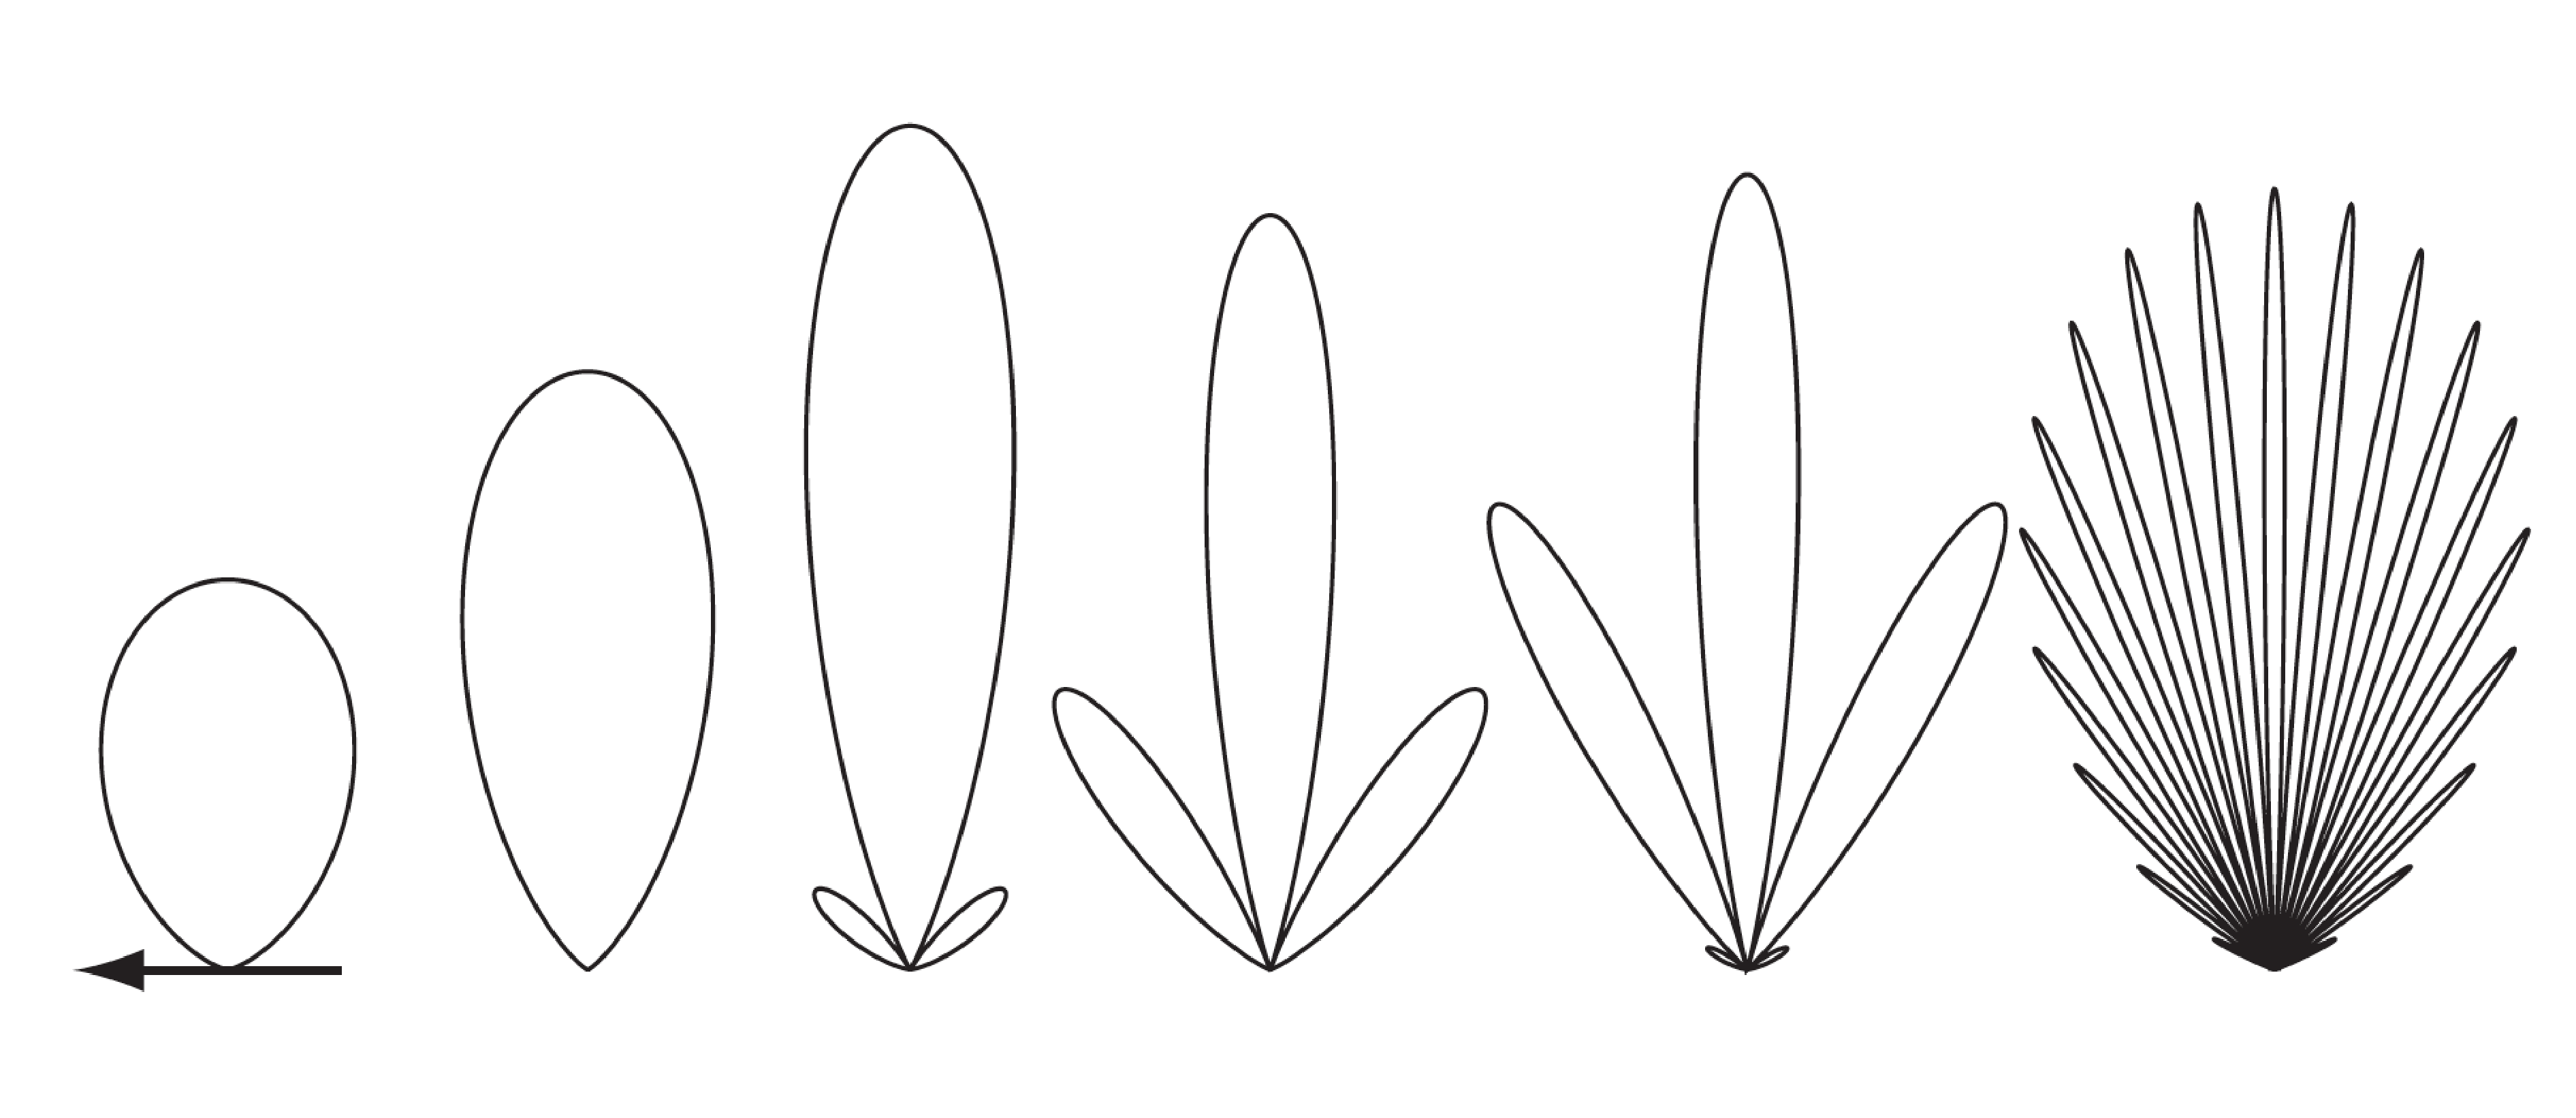
\includegraphics[width=0.8\textwidth]{two_atoms.pdf}
\end{center}
\caption[Radiation patterns for two dipoles]{Normalized radiation patterns $P(\theta;l)\sin\theta$ for the two dipoles for the distances between the dipoles $l=0,\pi,2\pi,3\pi,4\pi$, and $20\pi$ (left to right). These are a polar plots for $\theta\in[0,\pi]$,with the direction of the dipole and the $z$ axis denoted by the arrow in the $l=0$ graph.}
\label{TWOATOMS}
\end{figure}

As to the radiated power, the detuning from the single-atom resonance shifted by the co-operative effects is the true measure of resonance effects. We momentarily assume that this shift of reference point is implicit in the expressions of the energetics of the radiation, and simply replace $\Delta(\ell)\rightarrow\Delta$. On the other hand, if there were no co-operative effects or interference between the radiations of the two dipoles, the total radiated power would simply be twice the radiated power from one dipole under the same field. The ratio of these quantities
\beq
C = \frac{P_2}{2 P_1} = \frac{\gamma(\ell)[\Delta^2+\gamma^2]}{\gamma[\Delta^2+\gamma^2(\ell)]}
\eeq
is a reasonable measure of cooperativity, with $C=1$ applying to completely independent radiators.

The explicit expression follows immediately from Eq.~\eq{GAMMAL}. Since in the limit $\ell\rightarrow\infty$ we have $\gamma(\ell)\rightarrow\gamma$, we find $C\rightarrow1$ as expected. In the opposite limit $\ell\rightarrow0$ we have $\gamma(\ell)\rightarrow 2\gamma$, and the co-operativity depends in an essential manner on the detuning. If $|\Delta|\ll\gamma$, we have $C\simeq\half$. This means that on resonance the two atoms together radiate the same power as one single atom. On the other hand, with $|\Delta|\gg\gamma$, we have $C\simeq2$, and the two-atom sample radiates twice as much power as two independent atoms would. In fact, in this limit the radiated power can be expressed at all detunings as
\beq
P_2 = \frac{3 |E_0|^2}{2\{[\Delta/\gamma(\ell)]^2+1\}}\,,
\eeq
as if we had a single dipole with the dipole moment matrix element equal to $\sqrt2$ times the original dipole moment matrix element. Now, it is well known that on resonance the cross section for light scattering is independent of the dipole moment matrix element, so the cross section and scattered power are both independent of the dipole matrix element. On the other hand, far-off resonance the scattered power is in fact proportional to the square of the dipole matrix element times the linewidth, and as such is proportional to the fourth power of the matrix element. Hence, the power from two atoms is four times the power from one atom, or twice the power from two independent atoms. The $\ell\rightarrow0$ limit is fully compatible with the observation that the two atoms have merged into one and the dipole matrix element has been multiplied by $\sqrt2$, with the proviso   that, as a result of atom-atom interactions, there is a shift of the resonance that diverges in the limit $\ell\rightarrow0$.

There is an interesting little puzzle here as well: One would imagine that the when one simply joins the two atoms, the dipole moment matrix element should, perhaps, be twice the matrix element for a single atom, not multiplied by $\sqrt 2$. Granted, in quantum mechanics, when restricted to the state space of collective states that are invariant under the exchange of the two atoms, the factor in fact is $\sqrt2$. But here we have a completely {\em classical\/} situation. Does everything fit in?

For an answer, let us momentarily take a variation of the classical Lorentz mode for a dipole, namely two classical charged particles with charge $q$ moving in the $z$ direction. Both particles are bound to their equilibrium positions with assumedly immovable neutralizing charges so that there are restoring forces proportional to the square of the of natural frequency $\omega_0$ common to both of the oscillators. By a suitable choice of the origins of the coordinates, we make the equilibrium positions equal to zero. Nonetheless, we assume that in actuality the dipoles  sit back to back as in the example of the present section, and much closer than the wavelength of the driving light from one another. The fields from one dipole, the moving charge and the stationary "nucleus", then add up to a force that attempts to move the other charge in the same direction. We characterize this force by the frequency $\Omega$. Finally, we assume that both of the dipoles are driven by the same external field $E$ at the freqency $\omega$. The equations of motion for the positive-frequency components of the positions of the two charges are then
\bea
\ddot{z}_1 = -\omega_0^2 z_1+ \Omega^2 z_2 + \frac{qE}{2}e^{-i\omega t},\label{INDIVDIP1}\\
\ddot{z}_2 = -\omega_0^2 z_2+ \Omega^2 z_1 + \frac{qE}{2}e^{-i\omega t}\,.
\eea
In terms of the normal modes
\beq
\eta_\pm = \frac{1}{\sqrt 2} (z_1 \pm z_2)
\eeq
the equations of motion read
\bea
\ddot{\eta}_+ &=& -(\omega_0^2-\Omega^2)\eta_+ +\frac{qE}{\sqrt2} e^{-i\omega t},\label{COLLDIPP}\\
\ddot{\eta}_- &= &-(\omega_0^2+\Omega^2)\eta_-\,.
\eea
The resonance of the two modes $\eta_\pm$ are  shifted  in the opposite directions by the interaction between the dipoles. Besides, the ``nonradiating'' mode $\eta_-$ does not couple to the driving field at all. 

Let us now assume that there is some damping in the system that eventually leads to equilibrium, but which is otherwise negligible; for instance that we drive the dipoles off resonance. Then there is no excitation of the mode $\eta_-$. Moreover, a comparison of Eqs.~\eq{COLLDIPP} and~\eq{INDIVDIP1} with $\Omega=0$ shows that for the same driving field strength $E$ and for the same detuning of the frequency $\omega$ from the respective resonance frequencies $\sqrt{\omega_0^2-\Omega^2}$ and  $\omega_0$, the steady-state oscillation amplitude of the collective mode $\eta_+$ would be a factor of $\sqrt 2$ larger that the amplitude for a single dipole. This is ostensibly the $\sqrt 2$ for the collective response in quantum mechanics, but the normal modes are an auxiliary construct and as such have no a priori meaning in classical mechanics. We therefore consider the original displacement $z_1$ and $z_2$. These oscillate in phase and with the same amplitude as would one dipole, for the same detuning from resonance. The total radiated electric field from the two dipoles will thus be twice the field from one dipole and the radiated power is multiplied by four. Everything is as it should be.


\section{Radiation Power of Gaussian Clouds of Atoms}


\subsection{Continuous Medium}

For the more general problem of $N$-atom gases, let us start with a hypothetical model with continuous spatial distribution of atoms.

In terms of macroscopic electromagnetism, there is a monochromatic polarization of the sample
\beq
{\bf P}({\bf r},t) = \half\varrho({\bf r}) \,{\bf d}({\bf r})e^{-i\omega t} + {\rm c.c.}\,,
\eeq 
where $\varrho({\bf r})$ is the density of the sample  and $\bf d({\bf r})$ is the positive-frequency component of the eletcric dipole of an atom at the position $\bf r$. Taking the atoms  to reside around the origin of the coordinates, in the far field with $r\gg \lambda$ and $r\gg R$, the terms  $\propto 1/R^2$ and $\propto 1/R^3$ in Eq.~\eq{dipolarE} would vanish and the it gives the positive component of the field radiated by this polarization in the form
\bea
{\bf E}_R({\bf r})&\simeq&\frac{e^{ir}}{r} \int d^3r'\,e^{-i  \hat{\bf r}\cdot {\bf r}'}\varrho({\bf r}')
\, [\hat{\bf r}\times{\bf d}({\bf r}')]\times\hat{\bf r}\,;
\label{SCATFIELD}
\eea
$\hat{\bf r}={\bf r}/r$ is the unit vector that points from the source at $\simeq 0$ to the field point. 

For easy analysis, we model the density with a Gaussian,
\beq
\varrho({\bf r}) = \frac{3\sqrt3N}{2\sqrt2\pi^{3/2} R^3}\, e^{-\frac{3r^2}{2R^2}}\,,
\eeq
where $N$ is the atom number. In the limit $kR\gg1$ there will be a narrow cone of radiation around the direction of the incoming beam; let us denote the angle from the incident beam by $\theta$. The parametrization is chosen in such a way that the rms value of $|\br|$ equals $R$. 

For a tangible example, let us take a $\sigma_+$ circularly polarized plane wave propagating in the $z$ direction, writing
\beq
\bE_0(\br) = E_0\, e^{iz}\,\hat{\bf e}_+;\quad \hat{\bf e}_+=\frac{1}{\sqrt{2}}(\hat{\bf e}_x - i \hat{\bf e}_y)\,.
\label{incomingE}
\eeq
Accordingly, 
\bea
{\bf d}({\bf r})=\alpha\bE_0(\br)=\alpha E_0\, e^{iz}\,\hat{\bf e}_+;
\eea
Now we turn back to the radiated field:
\bea
{\bf E}_R({\bf r})&=&\frac{e^{ir}}{r}\int d^3r^{\prime} e^{-i\hat {{\bf n}} \cdot {\bf r}^{\prime}} \rho({\bf r^\prime}) [ \hat { \bf n} \times  {\bf d}({\bf r}^{\prime}) ]  \times \hat {\bf n}\nonumber\\
&=&\frac{3\sqrt{3}\alpha NE_0e^{ir}[ (\hat { \bf n} \times \hat{{\bf e}}_+)  \times \hat {\bf n}]}{2\sqrt{2}\pi ^{3/2}R^3r}\int d^3r^{\prime} e^{-i\hat {{\bf n}} \cdot {\bf r}^{\prime}}e^{iz}e^{\frac{-3r^{\prime2}}{2R^2}}\nonumber\\
&=&\frac{\alpha NE_0e^{ir-\frac{1}{3}R^2(1-\cos \theta)}}{r}[ (\hat { \bf n} \times \hat{{\bf e}}_+)  \times \hat {\bf n}].
\eea
The magnitude of the Poynting vector is 
\bea
S_C({\bf r})&=&\frac{|{\bf E}_R|^2}{8\pi}=\frac{\left|\alpha\right|^2N^2 E_0^2 e^{-\frac{2}{3}R^2(1-\cos \theta)}|(\hat { \bf n} \times \hat{\bf e}) \times \hat {\bf n} |^2}{8 \pi r^2} \nonumber\\
&=&\frac{\left|\alpha\right|^2N^2 E_0^2 e^{-\frac{2}{3}R^2(1-\cos \theta)} (1+\cos^2 \theta)}{16 \pi r^2};  
\eea
The total power of the radiation is readily obtained by
\bea
P_C&=&\int r^2 S_C({\bf r}) d^2\Omega\nonumber\\
&=&\frac{3\left|\alpha\right|^2N^2E_0^2\left[(4R^4-6R^2+9)-e^{-\frac{4R^2}{3}}(4R^4+6R^2+9)\right]}{32R^6}.
\eea
Here, the intensity of the observation light scales with the square of the atom number, $N^2$. This is similar to the important characteristic of superradiance. However, it's early for a conclusion now. Let us check a more realistic problem, where we have discrete atoms instead of a over simplified continuous medium.

\subsection{Independent Radiators}
Suppose we have collection of $N$ identical dipoles sitting at the positions ${\bf r}_i$ in the incoming field, and that each of these dipoles radiate a field ${\bf E}_i({\bf r})$ {\em independently\/} of one another, i.e., with no co-operative effects. The total dipolar field at the point ${\bf r}$ is then simply
\beq
{\bf E}_D({\bf r}) = \sum_i {\bf E}_i({\bf r})\,.
\eeq
Suppose we are in the far field when the Poisson vector is obviously radial and its absolute value is related in the same simple way to the square of the electric field as for a single dipole. The Poynting vector for the dipolar field then points radially outwards, and has the absolute value
\bea
S_D(\br) &=& \frac{1}{8\pi} \bE_D(\br)\cdot\bE_D^*(\br )\nonumber\\
&=& \frac{1}{8\pi} \sum_{i,j} \bE_i(\br)\cdot\bE_j ^*(\br)
\eea
It may be that the atoms, in fact, reside in some fixed configuration, but for a gaseous sample it is more physical to take them to have some random position distribution in space. We take the position of each atom to be a random variable independent of the positions of the other atoms, governed by same probability density function $f(\br)$. Then the average outward energy flux (over many samples of the gas) is given by
\bea
8 \pi\bar{S}_D &=&\left\langle
 \sum_{i\ne j} \bE_i(\br)\cdot\bE_j^*(\br)+\sum_i \bE_i(\br)\cdot\bE_i^*(\br)
\right\rangle\nonumber\\
&=&
 \sum_{i\ne j} \left\langle\bE_i(\br)\right\rangle
\cdot\left\langle\bE_j^*(\br)\right\rangle +
\sum_{i} \left\langle\bE_i(\br)\cdot\bE^*_i(\br)\right\rangle\nonumber\\
&=&N(N-1)|\left\langle \bE_i(\br)\right\rangle|^2 + N \left\langle\bE_i(\br)\cdot\bE^*_i(\br)\right\rangle\,.
\eea
The first term represents coherent scattering, as if the atom was spread out to a continuous dielectric material with the spatial shape specified by $f(\br)$. It arises from adding the fields of different radiators, and is essentially proportional to $N^2$. The second term $\propto N$ is for incoherent scattering, basically the sum of intensities radiated by the individual atom. It is present because the gas is not a continuous dielectric medium, but consists of discrete scatterers.

Incidentally, while this argument may not be as widely known as it deserves to be, it is far from new: Einstein used it to demonstrate the atomic (molecular) nature of matter when it was still under doubt. The blue sky comes from incoherent scattering. If air were a continuous dielectric medium, it would not scatter sunlight sideways, and the sky would be black.

For comparison purposes, we apply the same incoming light as in Eq.~\eq{incomingE} and the position distribution for the atoms is still taken to be Gaussian,
\beq
f(\br) = \frac{3\sqrt3}{2\sqrt2\,\pi^{3/2}R^3}\,e^{-\scriptstyle\frac{3r^2}{2R^2}}\,.
\eeq
Given the usual polarizability $\alpha$, the far field (the $1/r$ part of dipole radiation) averaged over the position of the atom, the absolute square of the former, and the  absolute square  of the field averaged over the positions give
\bea
\langle \bE_i(\br)\rangle &=& \alpha E_0 e^{ir-\hbox{$\frac{1}{3}$}R^2(1-\cos\theta)}[(\hat{\bf r}\times\hat{\bf e}_+)\times\hat{\bf r}]\,\frac{e^{ir}}{r},\\
|\langle \bE_i(\br)\rangle|^2 &=& \frac{|\alpha |^2| E_0|^2[3+\cos (2 \theta )] e^{\frac{2}{3} R^2 [\cos (\theta
   )-1]}}{4 r^2},\\
   \langle |\bE_i(\br)|^2\rangle &=& \frac{|\alpha |^2| E_0|^2[3+\cos (2 \theta )]}{4 r^2}\,.
\eea
The total radiated power then becomes
\bea
P_N&=&\frac{|\alpha|^2 |E_0|^2}{3}\Bigg\{
N(N-1)\frac{9\left[(4R^4-6R^2+9)-e^{-\frac{4R^2}{3}}(4R^4+6R^2+9)\right]}{32R^6}\nonumber\\
&&+N\Bigg\}\,.
\label{PN}
\eea

\begin{figure}[h!]
\begin{center}
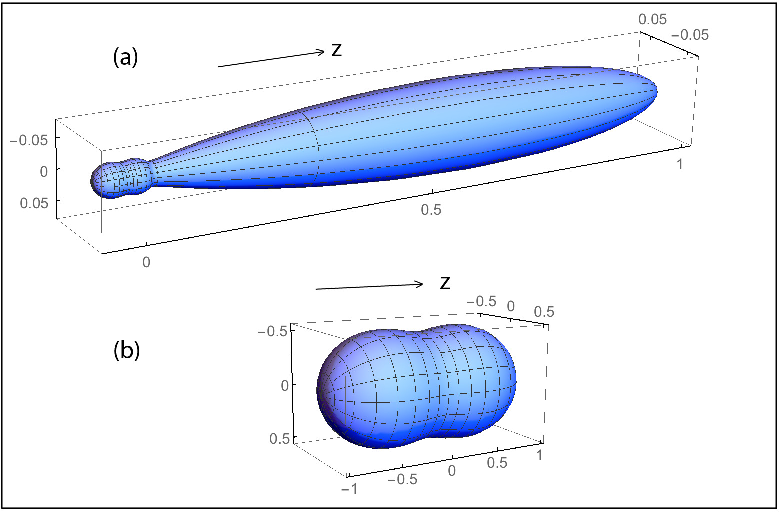
\includegraphics[width=\textwidth]{angular.pdf}
\end{center}
%\caption{Log-log plot of the total radiated power vs. the number of atoms from two types of models. $R$=1 and $\delta=600$ in both cases. The solid line is the result of Eq.~\eq{PN}. Ret dots denote the results from simulations.}
\caption{Normalized radiation patterns $P_N(\theta,R)\sin\theta$ for two Gaussian samples with $kR=10$ in (a) and $kR=0.1$ in (b). For both cases, the number of atoms $N=20$ and $\delta=600$.}
\label{ANGULAR}
\end{figure}


The main utility of these formulae is that they will serve as references to which to compare the numerical results. A few incidental results could be noted, however. As shown in Fig.~\eq{ANGULAR}, first, the intensity of the radiation in the forward direction, $\theta=0$, coherent and incoherent component, add up to exactly $N^2$ times the intensity from a single atom. The bigger the sample, the narrower the cone in the direction $\theta=0$ for coherent scattering. The sample acts as an antenna that directs the radiation in the forward direction. However, the total power decreases with increasing size of the cloud. Conversely, in the limit $R\rightarrow0$ the intensity in all directions is enhanced by a factor $N^2$, and of course so is the total power. People familiar with the Dicke cooperative regime might erroneously interpret such an enhancement as a cooperative phenomenon, which it is not since in this example we have simply added the fields from independent radiators.

%Last but not least, the difference between the continuous medium model and the independent radiators model in the total scattering power is given by
%\bea
%P_N-P_C&=&\frac{N\left|\alpha\right|^2E_0^2}{3}\nonumber\\
%&&\cdot\left\{1-\frac{9\left[(4R^4-6R^2+9)-e^{-\frac{4R^2}{3}}(4R^4+6R^2+9)\right]}{32R^6}\right\}
%\label{diffNandC}
%\eea

\subsection{Simulation of the scattered light power} 

When the dipolar fields from all the other radiators are taken into account, an analytical calculation for the total power is impractical and we have to turn to simulations. 

\begin{figure}[h!]
\begin{center}
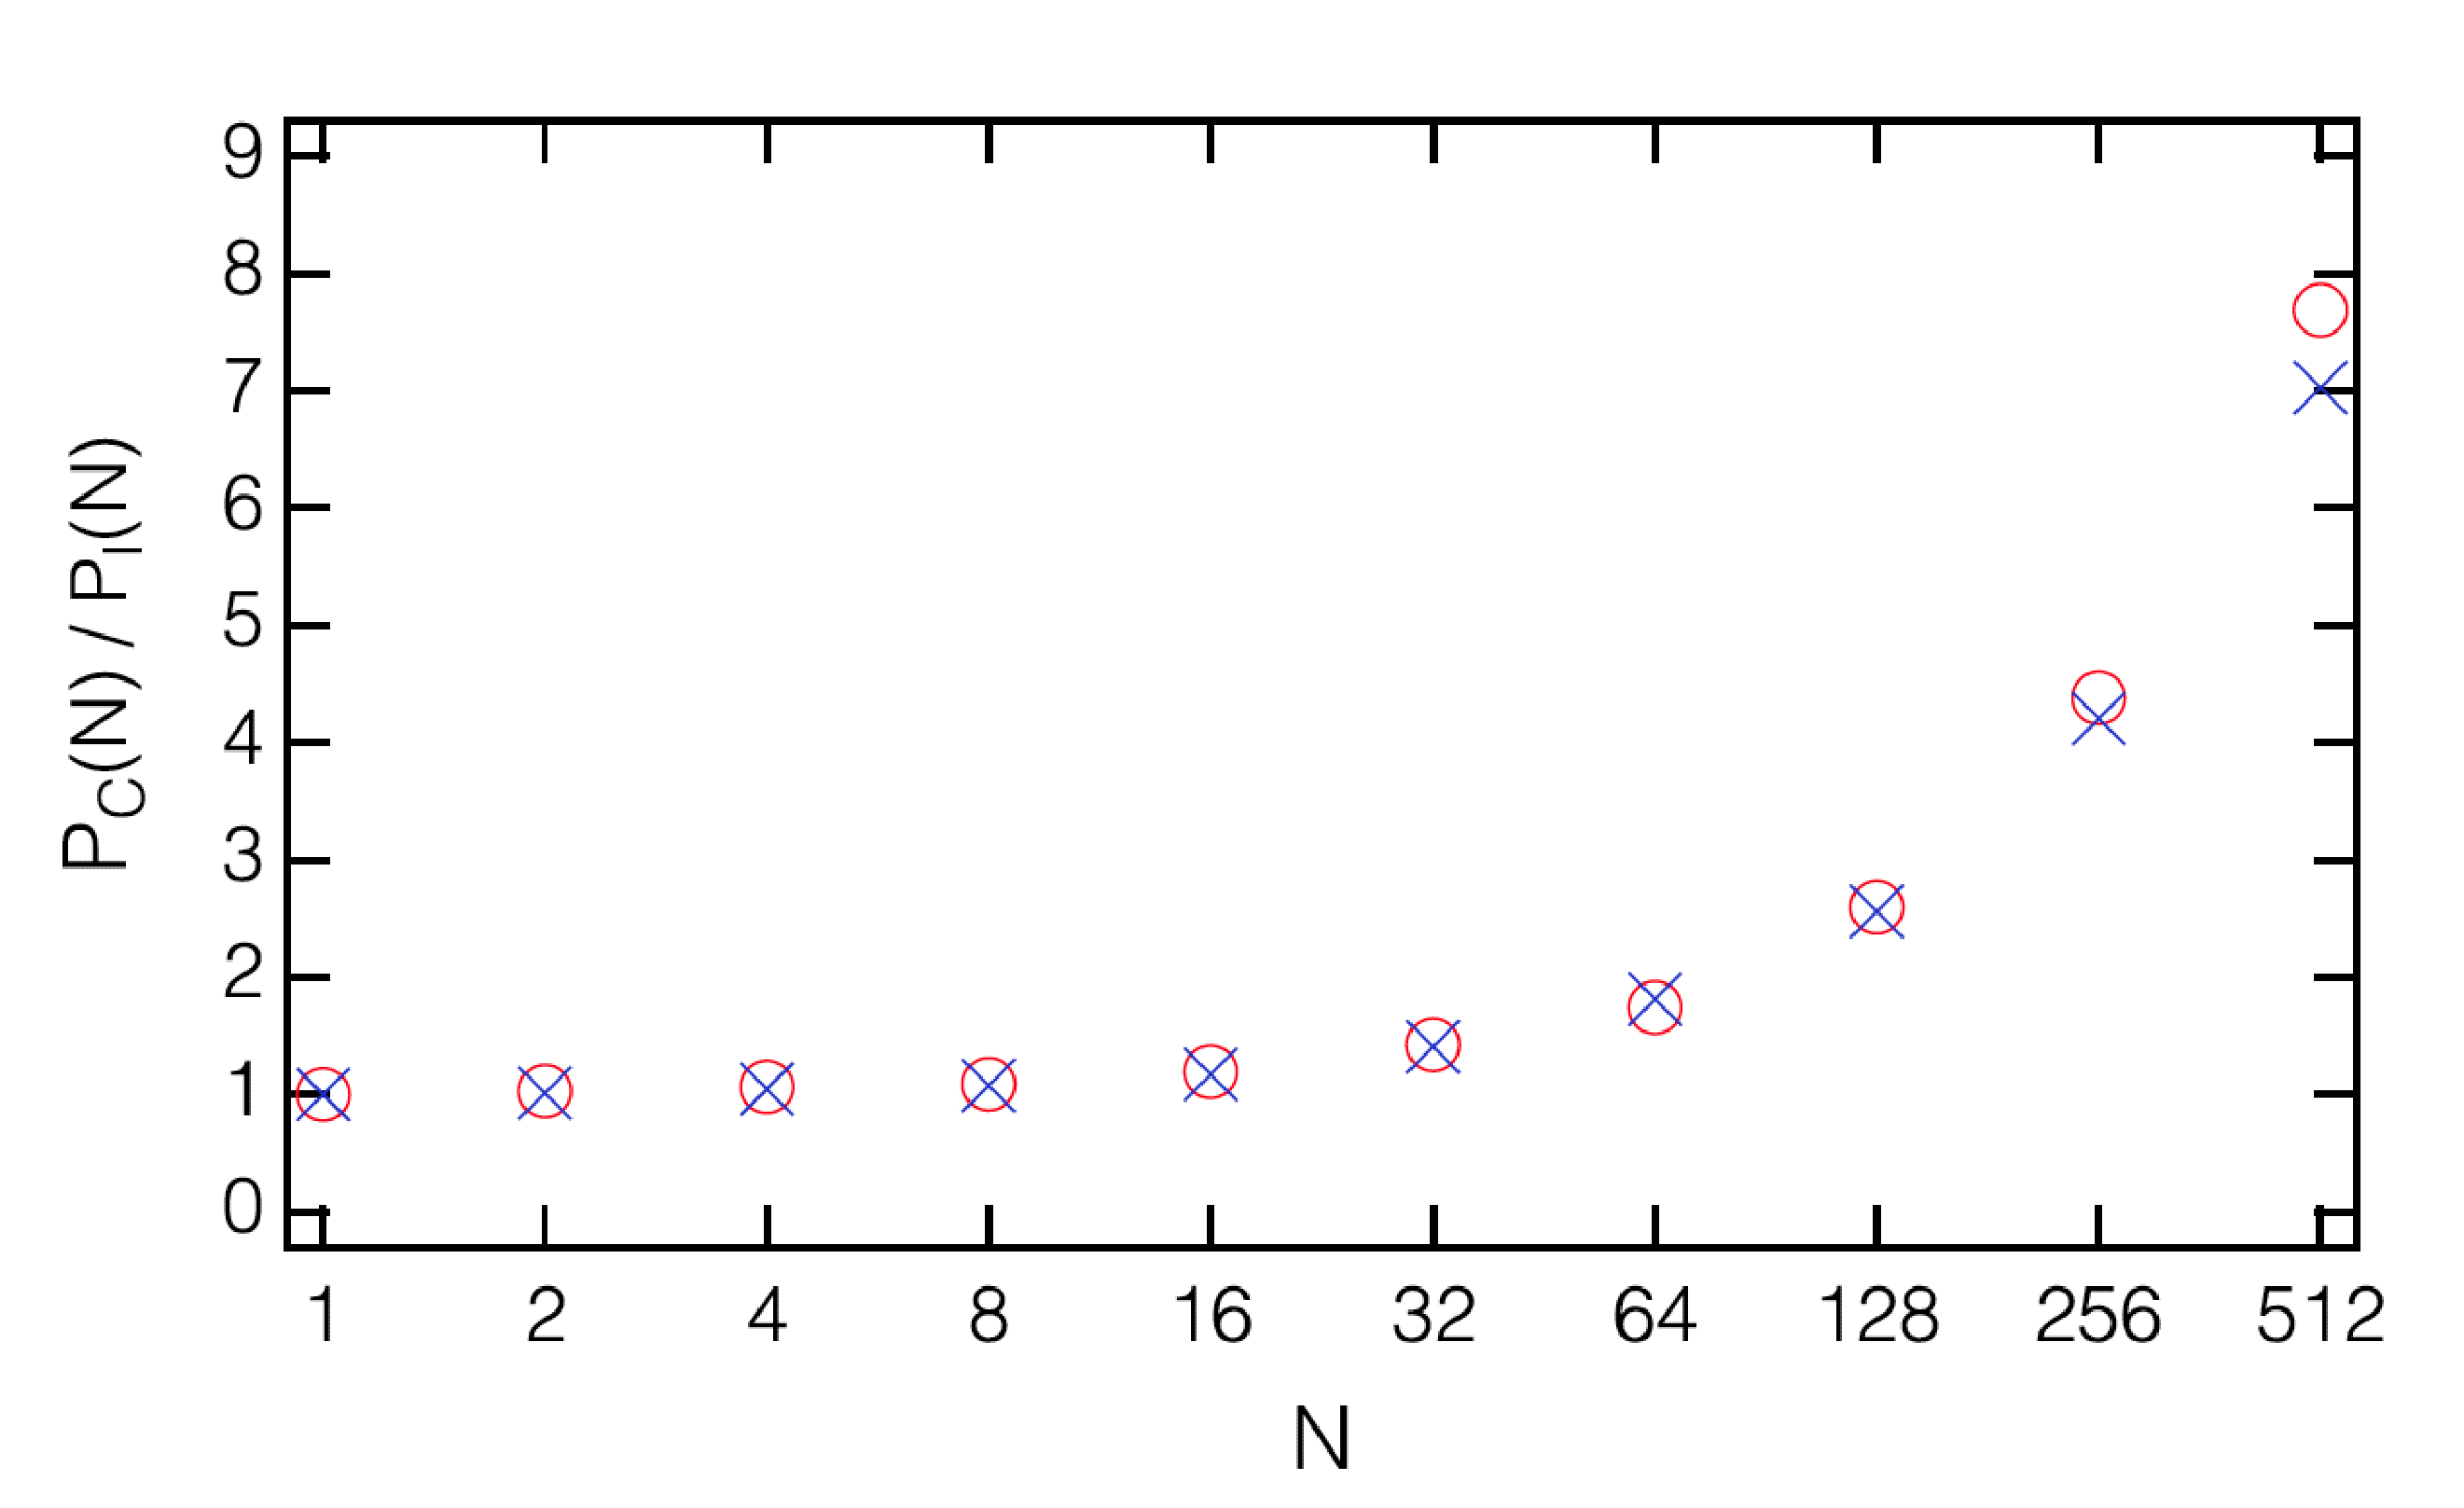
\includegraphics[width=\textwidth]{Pc_Pi.pdf}
\end{center}
%\caption{Log-log plot of the total radiated power vs. the number of atoms from two types of models. $R$=1 and $\delta=600$ in both cases. The solid line is the result of Eq.~\eq{PN}. Ret dots denote the results from simulations.}
\caption{Ratio of the numerically simulated scattered light power to the power from independently radiating atoms plotted for varying atom number $N$ for a Gaussian cloud with the rms radius $R$ satisfying $kR=10$. The detuning is varied in such a way that the estimated optical thickness through the center of the cloud is $10^{-2}$ for all $N$. The circles and crosses are for different signs of the detuning such that the cloud acts as eighteen focusing or a defocusing lens.}
\label{PCANDPN}
\end{figure}



We plot in Fig.~\eq{PCANDPN} the ratio of the numerically simulated collective power to the independent-atom power, $P_C(N)/P_I(N)$, for different number of the atoms $N$. Here the cloud radius give $kR=10$. While we vary the atom number and hence the density, we also vary the detuning in such a way that the estimated optical thickness for a ray going straight through the center of the could is $10^{-2}$, so that absorption of light should not be a major factor. We have both positive (circles) and negative (crosses) detunings that make the gas either a focusing or defocusing lens.

The surprise here is that by $N=128$ when the collectively scattered power already more than doubles the independent-atom power, the central density $n$ of the cloud gives the cooperativity parameter of only $\xi=n\lambdabar^3\sim 0.03$. Our hypothesis is that co-operation sets in much earlier than expected, and we suspect that the same applies elsewhere too.


%The solid line in Fig.~\eq{PCANDPN} reflects the analytical result of a Gaussian cloud of independent radiators as given by Eq.~\eq{PN} and the red scatters represents the results of  radiators with dipole-dipole interactions.  
 
%We notice that the total power with cooperativity exceeds at small atom numbers but the situation reverses at large $N$, where the gas radiates much less then one would expect according to Eq.~\eq{PN}. This is a clear signature of cooperativity (for the only difference in this two models is the presence of light rescattering between atoms. ?)

\section{Shifts of a Resonance Line of Gases in a Circular Disk}

Compared with the total radiated power, the spectroscopic evidence of cooperativity is of more interest to us. To observe this, we replace the Gaussian cloud with a gas sample evenly distributed in a circular-disk-shaped container. This geometry is vastly studied in recent theoretical and experimental research~\cite{PhysRevLett.108.173601}.

As previously mentioned, Lorentz-Lorenz or collective Lamb shifts are expected in a dense atomic sample as cooperative responses to light. 

We have also concluded in Chapter 3 that for a slab configuration, a uniform-density medium restricted to the interval $z\in [0,h]$ and a plane wave with the wave number $k=\omega/c$ propagating in the $z$ direction, in the limit of asymptotically small density $\rho$ of the medium, the absorption line is Lorentzian and is shifted by
\bea
\Delta_L=\Delta_{LL}-\frac{3}{4}\Delta_{LL}\left(1-\frac{\sin 2hk}{2hk}\right);\,\quad\Delta_{LL}=-\frac{\rho\mathcal{D}^2}{3\epsilon_0\hbar}
\label{LL_CLS}
\eea
from the atomic resonance. Here $\Delta_{LL}$, a redshift , is the standard LL shift, and $\Delta_L$ is the CLS as in Ref.~\cite{FRIEDBERG1973101}. In the present formulation the CLS is a combination of the LL shift and the etalon effect because of the reflections of light from the front and back surfaces of the sample. This is the CLS verified in the experiments~\cite{PhysRevLett.108.173601}.

The derivation of the CLS $\Delta_L$ in Ref.~\cite{FRIEDBERG1973101} and many other analyses such as in Ref.~\cite{PhysRevA.81.053821} are all built on a common foundation of mean-field theory. This approximation ignores the correlations between nearby atoms that might arise from dipole-dipole interactions, and as such is uncontrolled. This is why we will solve the light propagation problem using stochastic classical-electrodynamics simulations~\cite{PhysRevA.59.649,PhysRevE.69.026605,PhysRevLett.101.103602,1367-2630-14-5-055001,PhysRevA.86.031602,PhysRevB.86.085116,PhysRevB.86.205128,PhysRevA.88.033844}.

In the simulation, we have $N$ atoms fixed at positions $\br_i,\, i=1,\dots,N$, each with an assumedly isotropic polarizability $\alpha$, we find a closed set of linear equations given by Eq.~\eq{FEQ}. Having solved it numerically, we have the electric field amplitude everywhere as in Eq.~\eq{EF}.

The radius of the circular disk in our numerical experiments is $R=\sqrt{256/\pi}k^{-1}$, so that the area is $A=256k^{-2}$. We vary the thickness of the disk $h$ but keep the density $\rho=N/hA=2k^3$ constant in our examples, so the number of atoms $N$ varies accordingly. A circularly polarized plane wave comes in perpendicular to the pace of the disk. Analogous numerical experiments, although for different purposes, have been described in Refs.~\cite{1367-2630-14-5-055001,PhysRevA.86.031602}.  

We generate a number of random samples, from 64 to millions, of atomic positions evenly distributed inside the disk, compute the absorption as a function of the detuning $\Delta$ for each sample, and average the results. We express the final results in terms of optical thickness $D$ defined as $D=-\ln T$. The advantage is that in a medium that obeys Beer's law the line shape of optical thickness $D$ would be independent of the thickness $h$ of the sample. 

Fig.~\eq{HOMO_D} shows the optical thickness $D$ as a function of detuning $\Delta$ for the sample thicknesses $hk=0.25, 0.5, 1.0$ and $2.0$, with the corresponding atom numbers $N=128, 256, 512,$, and $1024$. For comparison we also give the predicted LL shift of this atom density as the dashed vertical line. The absorption lines are not Lorentzian. While the line broadens with increasing atom number and may be noticeably asymmetric, the maximum moves very little. The shift, if any, is at most a few percent of the LL shift. There is no manifest LL shift, nor a CLS.


\begin{figure}[h!]
\begin{center}
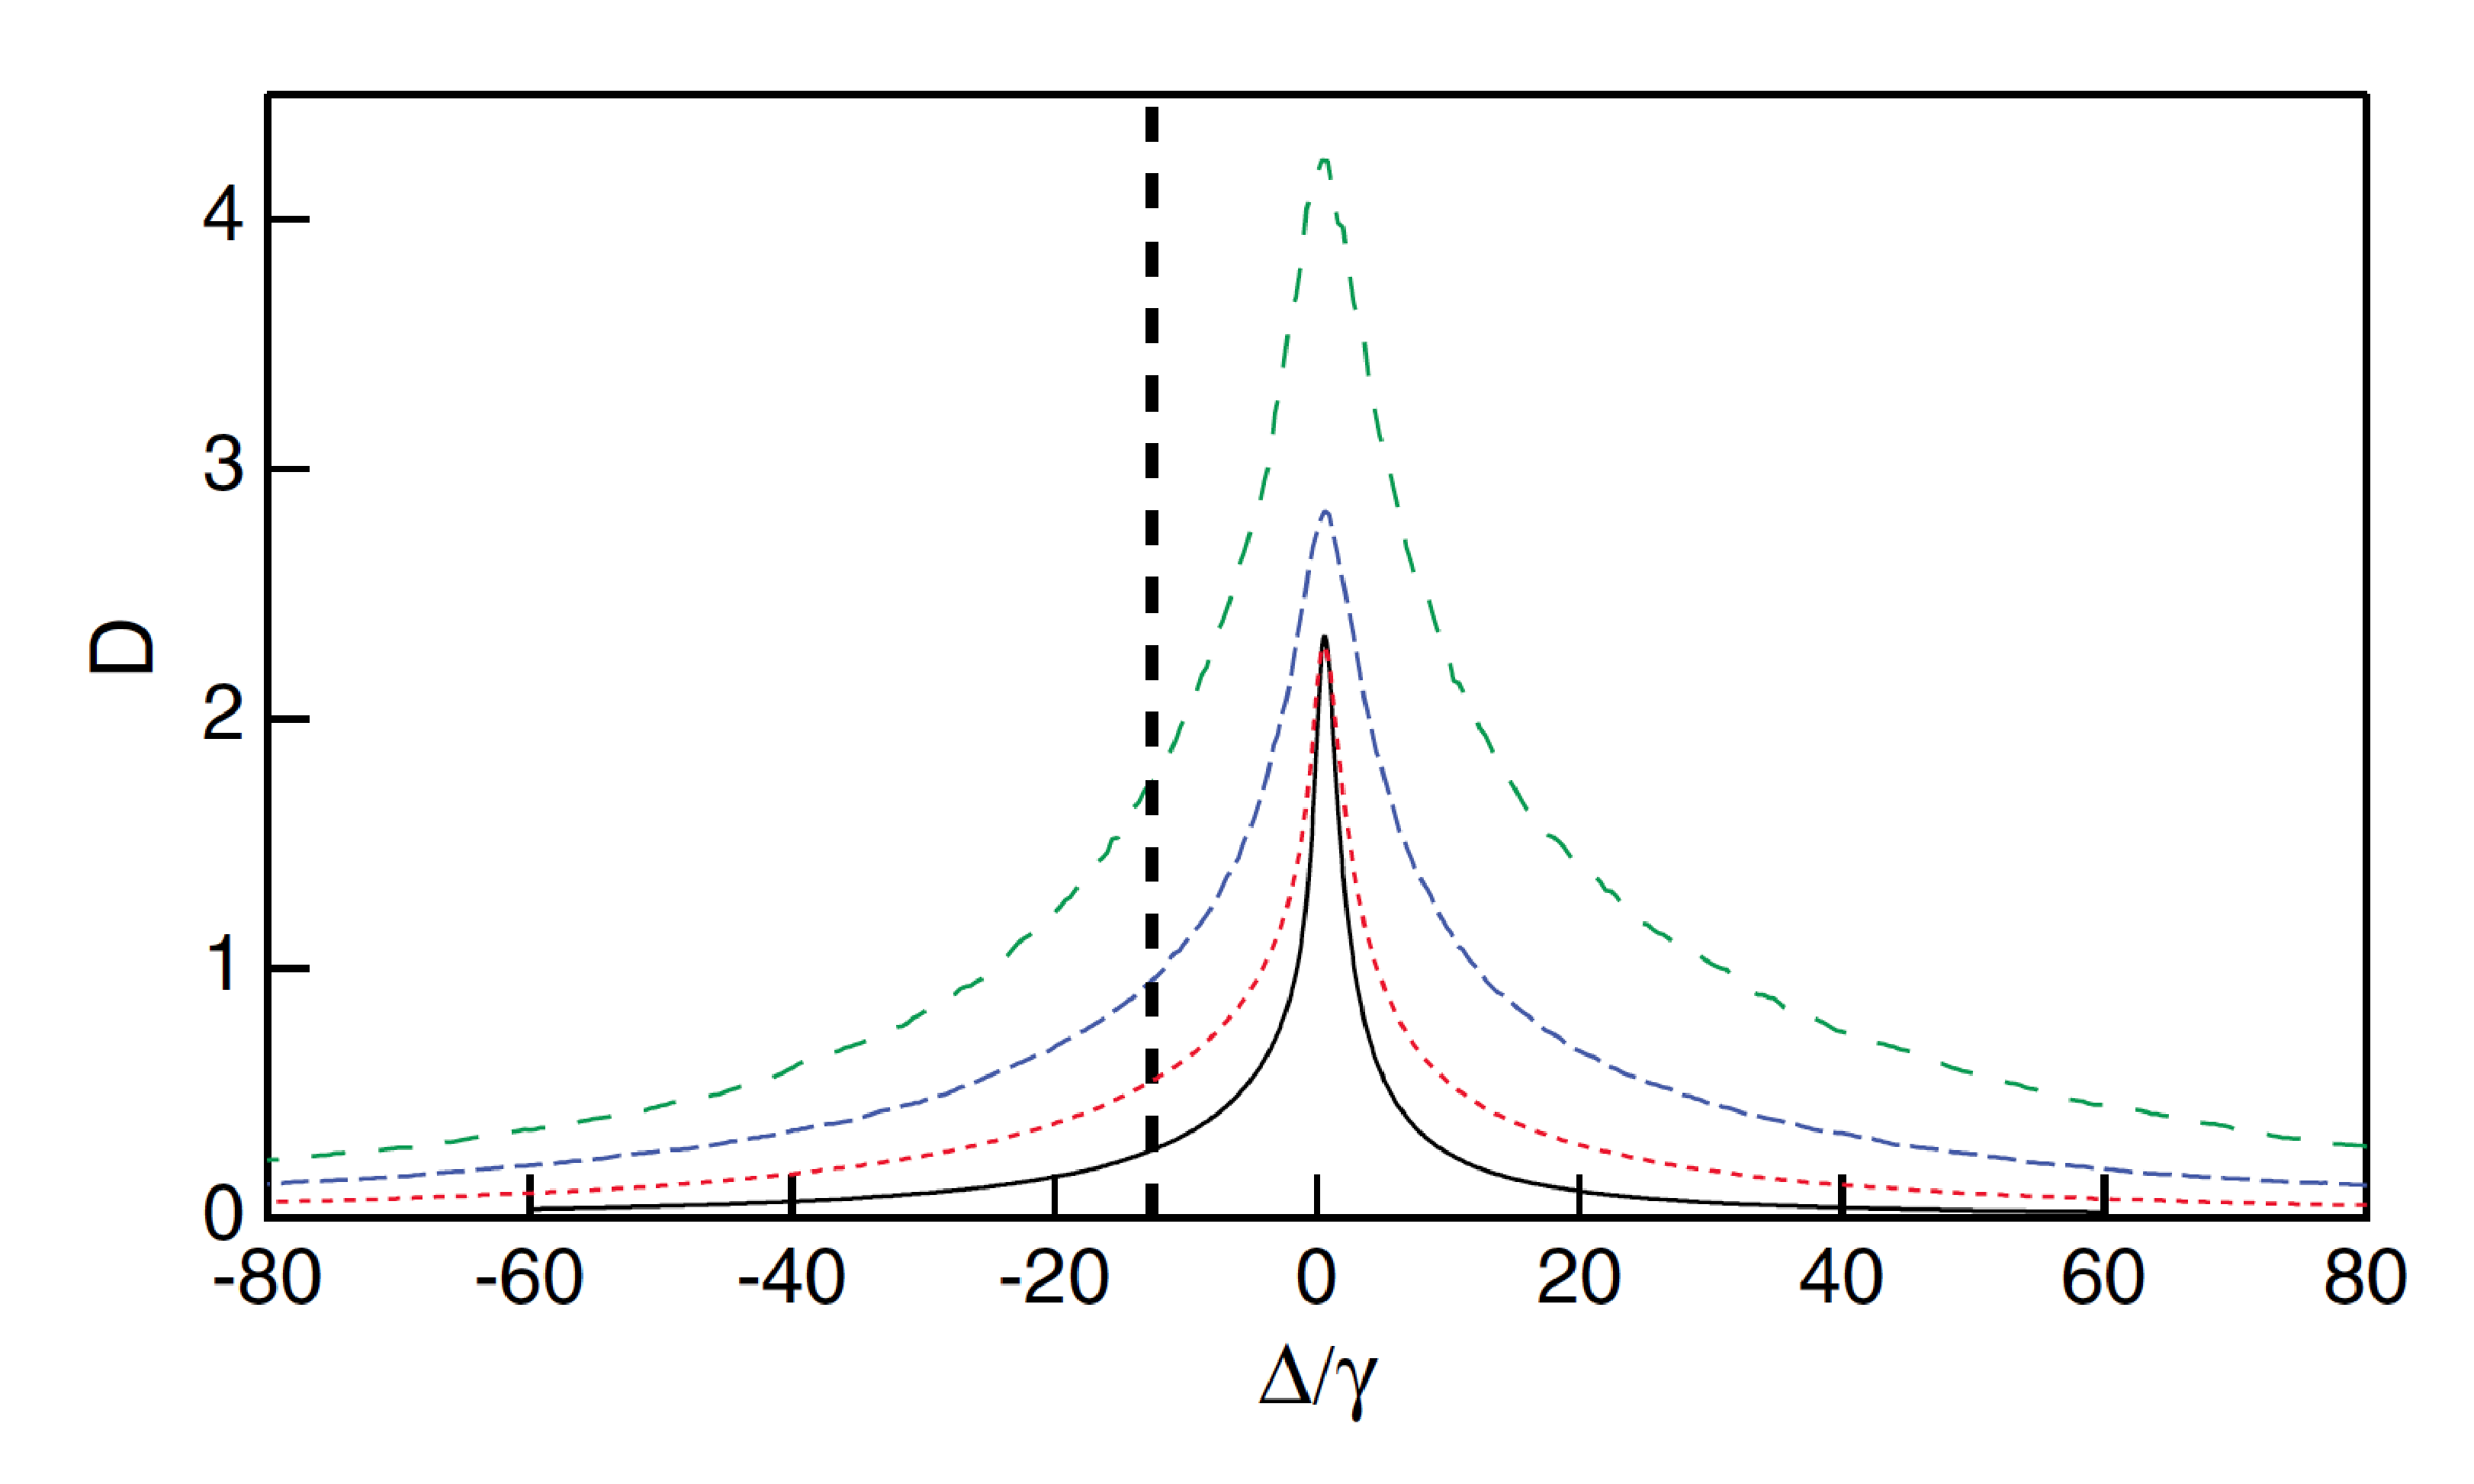
\includegraphics[width=\textwidth]{homo_D.pdf}
\end{center}
\caption{Optical depth $D$ versus detuning $\Delta$ in a homogeneously broadened sample for sample thicknesses $hk=0.25, 0.5, 1.0$, and $2.0$, from bottom to top; the corresponding atom numbers are $N=128, 256, 512,$ and $1024$. The dashed vertical line shows where the center of the line would be if the naive Lorentz-Lorenz shift applied.}
\label{HOMO_D}
\end{figure}

Note that the atoms are fixed in position, this configuration is obviously oversimplified. Therefore, although all correlations between atoms are included in the simulations, we do not observe the density dependent shifts, which are predicted from mean-field theory that ignores the correlations and verified by experiments.

Before introducing new factors into our simulations, such as atomic motions, we simply repeat the numerical experiments with stationary atoms in the circular disk, except that this time we assume that the resonance fequency of each atom is also shifted by a Gaussian random variable with zero mean and the rms value $\omega_D=100\gamma$, which could be interpreted as the effect of Doppler shift depends on the volocity of an atom.

An example spectrum is shown in Fig.~\eq{INHOMO_D}. The line shape has the appearance common in the spectroscopy of inhomogeneously broadened samples. Accordingly, we fit it with the Voigt profile $V(\Delta;\Gamma,\Omega_D)$, convolution of a Lorentzian with the HWHM width $\Gamma$ and a Gaussian with the rms width $\Omega_D$. 

\begin{figure}[h!]
\begin{center}
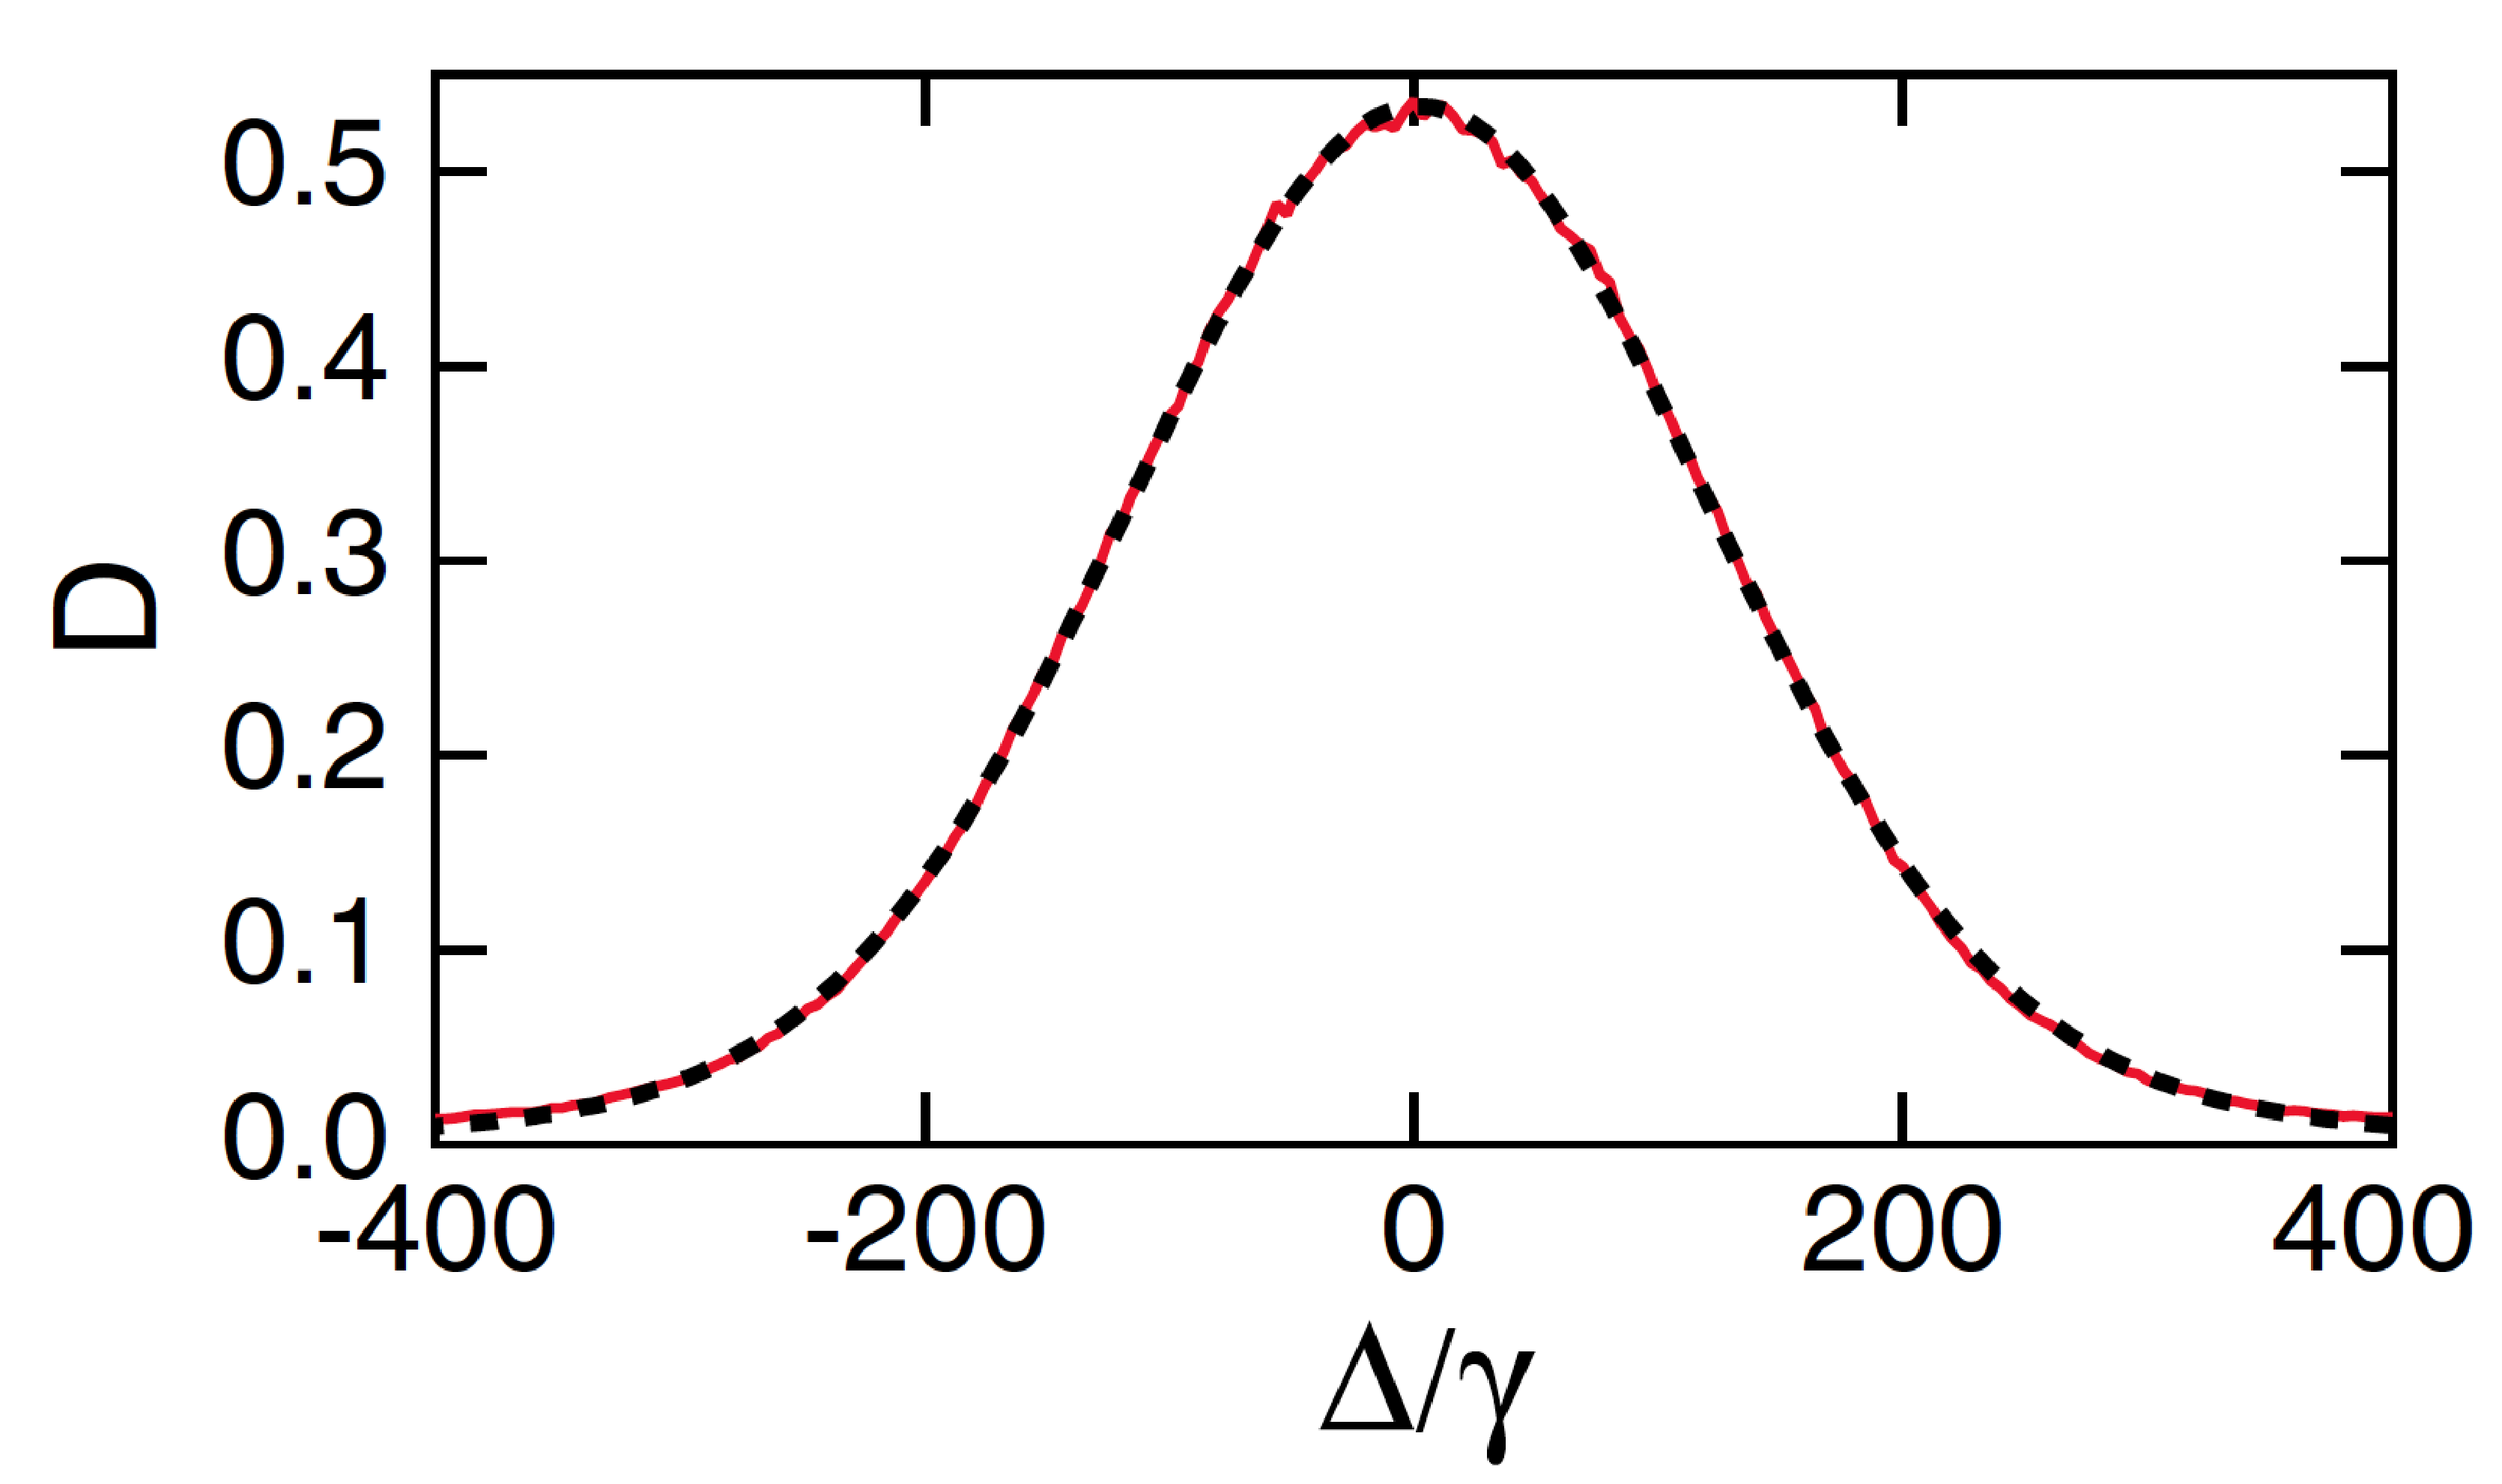
\includegraphics[width=\textwidth]{inhomo_D.pdf}
\end{center}
\caption{Optical depth of the sample $D$ with thickness $hk=1.5$, and, hence, $N=768$ atoms, as a function of the detuning for a sample with the inhomogeneous linewidth $\omega_D=100\gamma$. This numerical experiment (solid red line) is an average of 1024 samples, the fit with a Voige profile (dashed black line) has the parameters $s=2.15\gamma$, $\Gamma=17.74\gamma$, and $\Omega_D=112.83\gamma$.}
\label{INHOMO_D}
\end{figure}

We plot the shift of the resonance $s$ as a function of the thickness of the disk $h$ in Fig.~\eq{STATIC_CLS}, as filled circles. The shift tends to zero at small thicknesses. In this limit the physics becomes two dimensional, for a fixed three-dimensional density the relevant two-dimensional area density tends to zero, and eventually the toms mush radiate completely independently. 

We also plot the CLS, Eq.~\eq{LL_CLS}, as a solid line. Numerical data and theory show similar oscillations, albeit differing approximately by an additive constant. In Fig.~\eq{STATIC_CLS} we also plot as a dashed line the vertically translated version of the theory to fit the numerical data points with $hk\geq 1$. There was an additive term fitted to the experiments~\cite{PhysRevLett.108.173601}, too, before they gave an agreement with Eq.~\eq{LL_CLS}. The agreement of our numerical experiments with the theory is on a similar footing as in the real experiments.


\begin{figure}[h!]
\begin{center}
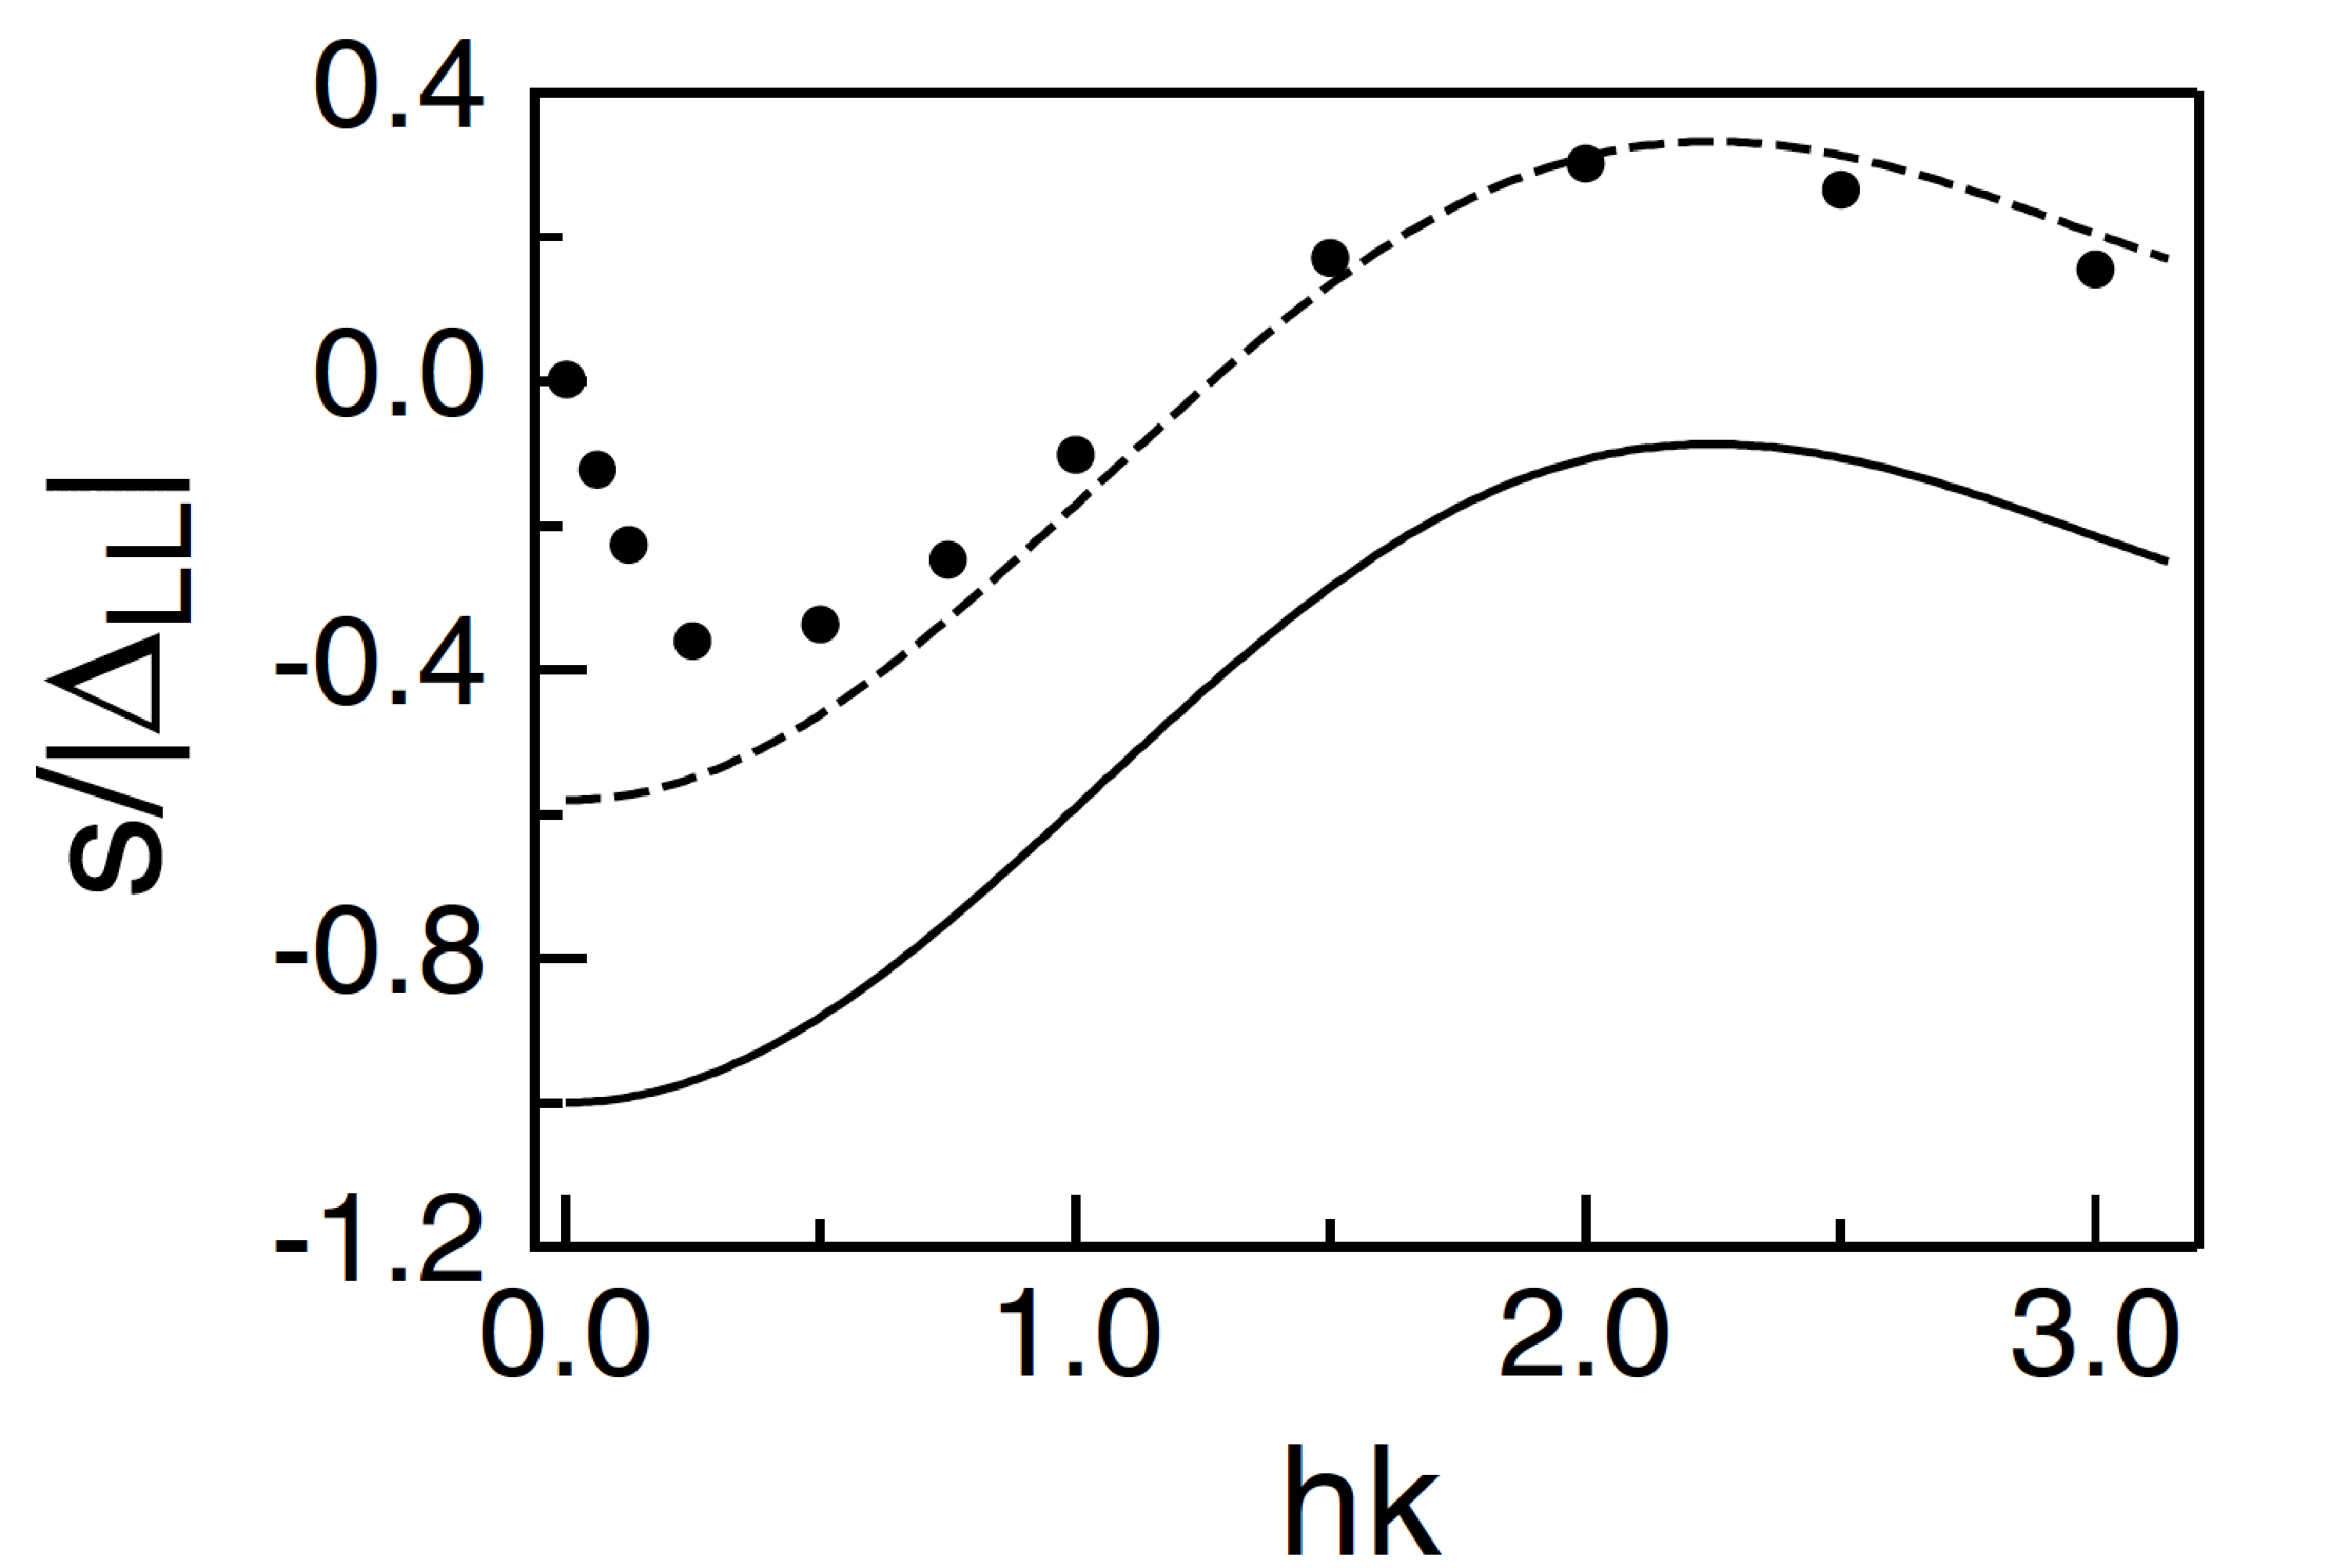
\includegraphics[width=\textwidth]{CLS_static.pdf}
\end{center}
\caption{The sift of the absorption line $s$ lotted as a function of the thickness of the sample $h$ as solid cricles. The statistical error bars are smaller than the size of the circles. Also shown as a solid line is the collective Lamb shift, Eq.~\eq{LL_CLS}, and as a dashed line a vertically translated version of Eq.~\eq{LL_CLS} fitted to the numerical data points with $hk\geq 1$.}
\label{STATIC_CLS}
\end{figure}


The inhomogeneous broadening apparently emphasizes mean-field physics at the expense of correlations between adjacent atoms.

Consider a two-atom sample of atom 1 and 2, with different resonance frequencies, hence, different polarizabilities $\alpha_1$ and $\alpha_2$, we can sketch a formal solution to Eq.~\eq{FEQ}. The field on atom 2 that is generated by the incident field and the light scattered from atom 1 yields
\bea
\bE(\br_2)&=&(1-\alpha_1\alpha_2\G\G)^{-1}[\cbE_0(\br_2)+\alpha_1\G\cbE(\br_1)]\nonumber\\
&=&\cbE_0(\br_2)+\alpha_1\G\cbE_0(\br_1)+\alpha_1\alpha_2\G\G\cbE_0(\br_2)+\dots.
\eea

The second line shows the first three terms of the expansion of $(1-\alpha_1\alpha_2\G\G)$, with $\G\equiv\G(\br_1-\br_2)=\G(\br_2-\br_1)$. The first term is the free field on atom 2; in the second term the free field excites atom 1, which sends its dipolar field back on atom 2; in the third term the free field excites atoms, which sends a dipolar field to excite atom 1, which sends a dipolar field back on atom 2. Further terms in the expansion come out the same way reflecting repeated photon exchanges between the atoms. Such recurrent scattering processes in which a classical wave scatters more than once by the same atom are responsible for the cooperative phenomena and the emergence of subradiant and superradiant resonanes~\cite{PhysRevA.55.513,PhysRevA.86.031602,PhysRevB.86.085116}

Let us now regard atom 2 as the spectator and imagine averaging over the position of atom 1. Upon averaging, the second term becomes the mean-field contribution radiated by an assumedly continuous polarization, and further terms represent repeated photon exchanges between the atoms. 

Next, add the inhomogeneous broadening $\omega_D$. To the order of magnitude, averaging over the resonant frequencies suppresses the polarizability by a factor or $\gamma/\omega_D$. Thus, the first nontrivial term in the expansion corresponding to the mean-field polarization gets suppressed by this small factor, and the higher terms by higher powers of the small quantity $\gamma/\omega_D$. Qualitatively, repeated photon exchanges are deemphasized because in such processes bothe the emitter and the absorber are off resonance.

Analogously, the transition from homogeneously broadened to inhomogeneously broadened phenomenology also takes place in a many-atom sample when the inhomogeneous broadening $\omega_D$ and the effective linewidth $\Gamma$ are comparable. This is, in fact, what we observe in the numerical experiments.

From classical-electordynamics simulations, we have found qualitative features in the optical response of a homogeneously broadened dense atomic sample that are at variance with the time-honored pictures of local-field corrections and collective Lamb shifts. However, an inhomogeneous broadening (random distribution of atomic resonance frequencies) restores the agreement with the traditional theory.

So far, the simulations are based on atoms fixed in position with an artificial inhomogeneous broadening. In the following chapter, real atomic motion will be introduced into the simulations.


\chapter{Gases of Moving Atoms}
In experiments, the atomic motion including collisions is another important factor that might impact the optical response of the gas. We have to face the possibility that the influence from the kinematics of atoms could be so remarkable that some cooperative effects may be more or less swept under the rug. Therefore, it is worthwhile to extend our simulations to moving atoms. 

Subsequent to the simulations on inhomoneneous broadened stationary atomic samples, we develop a program to deal with the atomic motions and the time evolution of dipole moments. 

Similarly, inhomogeneous broadening included in the simulations of moving atoms for it is a natural consequence of a thermal velocity distribution. Just as in the stationary-atom model, given a certain spacial distribution, we would be able to solve a closed set of linear equations to obtain the dipole moment of each atom.  However, in the moving-atom model, we integrate the equation of motion of each atom's dipole moment until the gas eventually reaches an equilibrium. During that time, atoms undergo free flight as well as elastic collisions with the container walls and other atoms. Accordingly, we find that some kinematic factors such as the frequency of collisions, may kick in to affect the simulation outcomes.

As expected, some results of stationary-atom simulations are inherited by moving-atom simulations, such as the dependence of collective Lamb shift on the sample thickness. Beyond that, some new features that do not exist in stationary-atom model could emerge. For instance, a typical Dicke narrowed lineshape~\cite{PhysRev.89.472} is observed. This is not surprising. After all, in reality, atoms are not stationary and Dick narrowing has been indeed observed.

However, contrary to what one might predict, as the gas density rises, the width of the Dick narrowed central peak is increasing. This is quite unlike what would happen in a hypothetical gas of independent atoms, wherein the higher density would reduce the linewidth. We attribute this broadening to the strong dipole-dipole interactions between the atoms, or from an overall perspective, the cooperative response of the gas to light. 

The following discussion is constructed similarly as last chapter of stationary atoms. We will start from the analysis of one single moving atom, extend to many independent atoms and finally focus on atoms with dipole-dipole interactions. Of course, all the calculations and simulations are done in a circular slab.

\section{Calculation of A One-atom Gas}
In our model of discrete dipolar radiators, Eq.~\eq{CORE} can be specified so that it describes the time evolution of each atom's dipole moment. For the $n$th atom located at $\mathbf{r}_n$, we have
\bea
\dot{\mathbf{d}}(\mathbf{r}_n)&=&(i\Delta-\gamma)\mathbf{d}(\mathbf{r}_n)+i\zeta\mathbf{\mathcal{E}}_0(\mathbf{r}_n)+i\zeta\sum_{m\neq n}\mathsf{G}(\mathbf{r}_n-\mathbf{r}_m)\mathbf{d}(\mathbf{r}_m).
\label{DIPOLEEQ}
\eea
As before, $\Delta=\omega-\omega_0$ is the detuning from the atomic resonance $\omega_0$, $\gamma$ is the HWHM line width of the transition, $\zeta=\mathcal{D}^2/\hbar$ and $\mathcal{D}$ is the dipole matrix element and $\mathbf{\mathcal{E}}_0$ is the electric field of the driving light if the matter were absent. $\mathsf{G}(\mathbf{r}_n-\mathbf{r}_m)$ is the dipole field propagator from the atom at $\mathbf{r}_m$ to the atom at $\mathbf{r}_n$.

It is worth reminding that atomic motion is taken into account in our model, hence $\mathbf{r}_n$ is actually a function of time and coordinates change with time as the atoms move.

The first term on the right hand side of Eq.~\eq{DIPOLEEQ} comes from the damped free evolution of the atomic polarization. The second and the third terms, respectively, correspond to the polarization induced by the incident light and the scattered light from all the other atoms. Apparently, if the left hand side of Eq.~\eq{DIPOLEEQ} equals zero, this equation would be reduced to a steady state as given by Eq.~\eq{STEADY}.

All the calculations and simulations we present below are all done with these universal configurations:


First, the gas sample is inside a circular disk with thickness $h$ and radius $R$. For convenience, the disk is placed so that its axis is used as the $z$ axis, and the body center is the coordinate origin.

Second, the incident light is represented by $\mathcal{E}_0(\mathbf{r})=E_0\,\hat{\mathbf{e}}\,e^{i\mathbf{k}\cdot\mathbf{r}}$. It is circularly polarized and the propagating in the $+z$ direction.
\bea
\hat{\mathbf{e}}=\{\frac{1}{\sqrt{2}},\frac{i}{\sqrt{2}},0\}, \, \mathbf{k}=\{0,0,1\}.
\eea

Third, the absorption spectrum is investigated by calculating the optical thickness $D$ of the sample, as defined in Ref~cite{0953-4075-44-19-195006}. Details will be given later.

Finally, the units we use are the same as for stationary atoms:
\bea
k=c=\hbar=\frac{1}{4\pi\epsilon_0}=1,
\eea 
and linewidth of the transition $\gamma$ and dipole matrix element $\mathcal{D}$ are still related by 
\bea
\mathcal{D}=\sqrt{\frac{3\gamma}{2}}.
\eea

\subsection{Dipole Evolution of the Atom}
If the gas consists of only one atom, Eq.~\eq{DIPOLEEQ} can be reduced to a nonhomogeneous first-order ODE:
\bea
\dot{\mathbf{d}}(t)+(1-i\delta)\mathbf{d}(t)=i\frac{3}{2}\mathcal{E}_0(t)=i\frac{3}{2}E_0\,\hat{\mathbf{e}}\,e^{i\mathbf{k}\cdot\mathbf{r}(t)},
\label{SINGLEEQ}
\eea
where $\delta=\Delta/\gamma$ and the dependence on position is expressed in the form of a dependence on time. 

For $\mathbf{k}=\{0,0,1\}$, we readily have $\mathbf{k}\cdot\mathbf{r}(t)=z(t)=z_0+v_zt$. Thus, the radial components of the initial position and the velocity have no impact on the evolution. So we need not concern with the collision between the atom and the lateral surface of the disk at all. As we will see later, even $z_0$ does not matter either. Therefore, we would not hesitate to endow the atom with $\mathbf{r}_0=\{0,0,-h/2\}$ and $\mathbf{v}_0=\{0,0,v\}$ to carry out our calculations. This atom is sufficient to represent all the atoms that have the same axial speed. Here, $v$ must be positive because the atom is initially at $z=-h/2$, the atom has to be moving in the $+z$ direction.

With the given assumptions, we have $\mathbf{d}_0=-\frac{3}{2(i+\delta)}E_0e^{-i\frac{h}{2}}\hat{\mathbf{e}}$ as the initial dipole moment for the evolution. As a matter of fact, the equilibrium state that the system would reach after a large number of collisions is independent of the initial state. Anyway, given $\bf{d}_0$, the solution to Eq.~\eq{SINGLEEQ} is
\bea
d(t)&=&-\frac{3E_0}{2(i+\delta-v)}e^{i(-h/2+vt)}\left[1-e^{-t+i(\delta-v)t}\right]+e^{-t+i\delta t}d_0
\label{SINGLESOL}
\eea
Note that we do not use the bold font any more because the dipole moment always has the same polarization as the incoming electric field, so $\hat{\mathbf{e}}$ can be eliminated in the equation and every thing now is scalar.

Obviously, the first term in Eq.~\eq{SINGLESOL} depends on the velocity and the instantaneous electric field at the ever-changing position of the atom. The second term is the damping of the initial state. In free space, as time tends to infinity, the dipole moment would asymptotically approach
\bea
d(t\to\infty)=\alpha(v)E_0e^{i(-h/2+vt)},
\eea
where $\alpha(v)\equiv-\frac{3}{2(i+\delta-v)}$ is the Doppler-shifted polarizability of the atom with speed $v$.

If the atom is restricted in a circular disk region so it experiences elastic collisions at $z=\pm h/2$, the direction of the velocity reverses after each collision. The time interval between any two successive collisions  is $h/v$. When the first collision happens at $z=h/2$, the dipole becomes
\bea
d_1\equiv d(t=\frac{h}{v})&=&\alpha(v)E_0 e^{ih/2}\left[1-e^{-\frac{h}{v}+i(\delta-v)\frac{h}{v}}\right]+e^{-\frac{h}{v}+i\delta \frac{h}{v}}d_0.
\eea

$d_1$ would in turn serve as the initial state to obtain the dipole at the second collision $d_2$. Note that this time $v$ is replaced by $-v$ for the atom would bounce back after the first collision:
\bea
d_2&=&\alpha(-v)E_0e^{-ih/2}\left[1-e^{-\frac{h}{v}+i(\delta+v)\frac{h}{v}}\right]+e^{-\frac{h}{v}+i\delta \frac{h}{v}}d_1\nonumber\\
&=&\alpha(-v)E_0e^{-ih/2}\left[1-e^{-\frac{h}{v}+i(\delta+v)\frac{h}{v}}\right]+\alpha(v)E_0e^{ih/2}\left[1-e^{-\frac{h}{v}+i(\delta-v)\frac{h}{v}}\right]e^{-\frac{h}{v}+i\delta \frac{h}{v}}\nonumber\\
&&+(e^{-\frac{h}{v}+i\delta \frac{h}{v}})^2d_0\nonumber\\
&=&d_+q+d_-+q^2d_0.
\eea

Here we have defined
\bea
d_+&=&\alpha(v)E_0e^{ih/2}\left[1-e^{-\frac{h}{v}+i(\delta-v)\frac{h}{v}}\right],\nonumber\\
d_-&=&\alpha(-v)E_0e^{-ih/2}\left[1-e^{-\frac{h}{v}+i(\delta+v)\frac{h}{v}}\right], \nonumber\\
q&=&e^{-\frac{h}{v}+i\delta \frac{h}{v}}
\eea
for an even more compact notion.

Now we can inductively write out the dipole moment at the $n$th collision as 

\begin{subequations}
\begin{numcases}{d_n=}
d_+\sum_{k=0}^{\frac{n-1}{2}}q^{2k}+d_-\sum_{k=0}^{\frac{n-3}{2}}q^{2k+1}+q^nd_0, &($n$ is odd and $n\geq 3$) \\
 \nonumber\\
d_+ \sum_{k=0}^{\frac{n-2}{2}}q^{2k+1}+d_- \sum_{k=0}^{\frac{n-2}{2}}q^{2k}+q^nd_0. &($n$ is even and $n\geq 2$)
\end{numcases}
\end{subequations}
Since $\left|q\right|<1$, the summations converge as $n\to\infty$ so that:
\begin{subequations}
\begin{numcases}{d_{n\to\infty}=}
\frac{d_++qd_-}{1-q^2}, \, & \textrm{(if $n$ is odd)}\label{FINAL1}\\
\nonumber\\
\frac{qd_++d_-}{1-q^2}. \, & \textrm{(if $n$ is even)}\label{FINAL2}
\end{numcases}
\end{subequations}

If we wait long enough, the time evolution of the dipole moment would eventually develop into an oscillation between the states of~\eq{FINAL1} and~\eq{FINAL2}, when the system reaches the equilibrium. Namely, at equilibrium, the dipole moment is equal to ~\eq{FINAL1} when the atom arrives at the base at $z=h/2$ and equal to ~\eq{FINAL2} when it is at $z=-h/2$.

Between the two bases, the dipole moment still evolves according to Eq.~\eq{SINGLESOL}. The oscillation of the dipole moment is synchronized with the kinematic oscillation. The period of both oscillations equals the duration of a round trip between the two bases, which is $2h/v$.

Consider the dipole moment in just one period, if we zero the timer when the atom is at $z=-h/2$, in the first half period the dipole moment is given by
\bea
d_{F}(t)&=&\alpha(v)E_0e^{ih/2}\left[1-e^{-t+i(\delta-v)t}\right]+q(qd_++d_-)\frac{1}{1-q^2}.
\label{FORWARD}
\eea

We zero the timer again when the atom reaches $z=h/2$, after that, during the return trip, the dipole is
\bea
d_{B}(t)&=&\alpha(-v)E_0e^{-ih/2}\left[1-e^{-t+i(\delta+v)t}\right]+q(d_++qd_-)\frac{1}{1-q^2}.
\label{BACKWARD}
\eea

Combining Eq.~\eq{FORWARD} and Eq.~\eq{BACKWARD}, we are able to write out the dipole moment at any time within one period:
\begin{numcases}{d(t)=}
d_F(t), & (for $0\leq t\leq  h/v$)\nonumber\\
d_B(t-h/v). & (for $h/v \leq t \leq 2h/v)$
\label{BACKFORTH}
\end{numcases}

\subsection{The Optical Thickness}
Now let's investigate the absorption spectrum by calculating the optical thickness $D=\ln\left|\tau\right|^{-2}$, as defined in Ref.~\cite{0953-4075-44-19-195006}.  

First of all, Eq.~\eq{BACKFORTH} is actually an explicit function of $h$, $v$, $\delta$ and $t$. So we write it as $d(h,v,\delta,t)$.

For a single atom as above, the transmission coefficient
\bea
\tau_1=1+\frac{2ie^{-iz(t)}d(h,v,\delta,t)}{R^2E_0},
\eea
where $z(t)$ is the position of the atom at time $t$. 

The optical thickness $D_1$ is
\bea
D_1(h,v,\delta,t)&=&\ln\left|\tau_1\right|^{-2}=-\ln\left|\tau_1\right|^2=-\ln(\tau_1\tau_1^*)\nonumber\\
&=&-\ln\Bigg\{1+2\,\mathfrak{R}\left[\frac{2ie^{-iz(t)}}{R^2}\frac{d(h,v,\delta,t)}{E_0}\right]\nonumber\\
&&+\left|\frac{2ie^{-iz(t)}}{R^2}\frac{d(h,v,\delta,t)}{E_0}\right|^2\Bigg\}.
\eea

For $R\gg1$, we have the approximation such that
\bea
D_1(h,\delta,v,t)&\approx&-\ln\left(1+2\,\mathfrak{R}\left[\frac{2ie^{-iz(t)}}{R^2}\frac{d(h,v,\delta,t)}{E_0}\right]\right)\nonumber\\
&\approx&-\frac{4}{R^2E_0}\mathfrak{R}\left[ie^{-iz(t)}d(h,v,\delta,t)\right].
\label{APPROX}
\eea

As we discussed in Sec. II, $z(t)$ and $d(h,v,\delta,t)$ are oscillating in phase, so the time average of the optical thickness can be calculated by integrating the whole term in the square brackets over a round trip of the atom and dividing the result by $2h/v$, as below.
 \bea
\bar{D}_1(h,v,\delta)&=&-\frac{4}{R^2E_0}\mathfrak{R}\left[\frac{v}{2h}\int_0^{\frac{2h}{v}} ie^{-iz(t)} d(h,v,\delta,t)dt\right]\nonumber\\
&=&\frac{4}{R^2}\mathfrak{R}\Bigg\{\frac{3v^3\left[coth(\frac{h-ih\delta}{v})-\cos(h)csch(\frac{h-ih\delta}{v})\right]}{h(i+\delta-v)^2(i+\delta+v)^2}\nonumber\\
&&-\frac{3(1-i\delta)}{2(i+\delta-v)(i+\delta+v)}\Bigg\}.
\label{THEORYD}
\eea

As a final step, we hypothesize an ensemble consisting of an infinite number of one-atom gas samples, over which the atom's axial velocity obeys a Gaussian distribution and the rms axial velocity (i.e. the standard deviation) equal $u$. Then a formal absorption spectrum is given by:
\bea
D_1(h,u,\delta)=\int_{-\infty}^{\infty}\bar{D}_1(h,v,\delta)\frac{e^{-\frac{v^2}{2u^2}}}{\sqrt{2\pi}\,u}dv.
\label{ONEATOMSPECTRUM}
\eea

According to Eq.~\eq{ONEATOMSPECTRUM}, given certain $h$ and $u$ values, we numerically calculate and plot $D_1$ versus $\delta$ in  Fig.~\eq{SINGLESPECTRUM}. The lines are calculation results and the scatters stand for the simulation outcomes.
\begin{figure}[h!]
\begin{center}
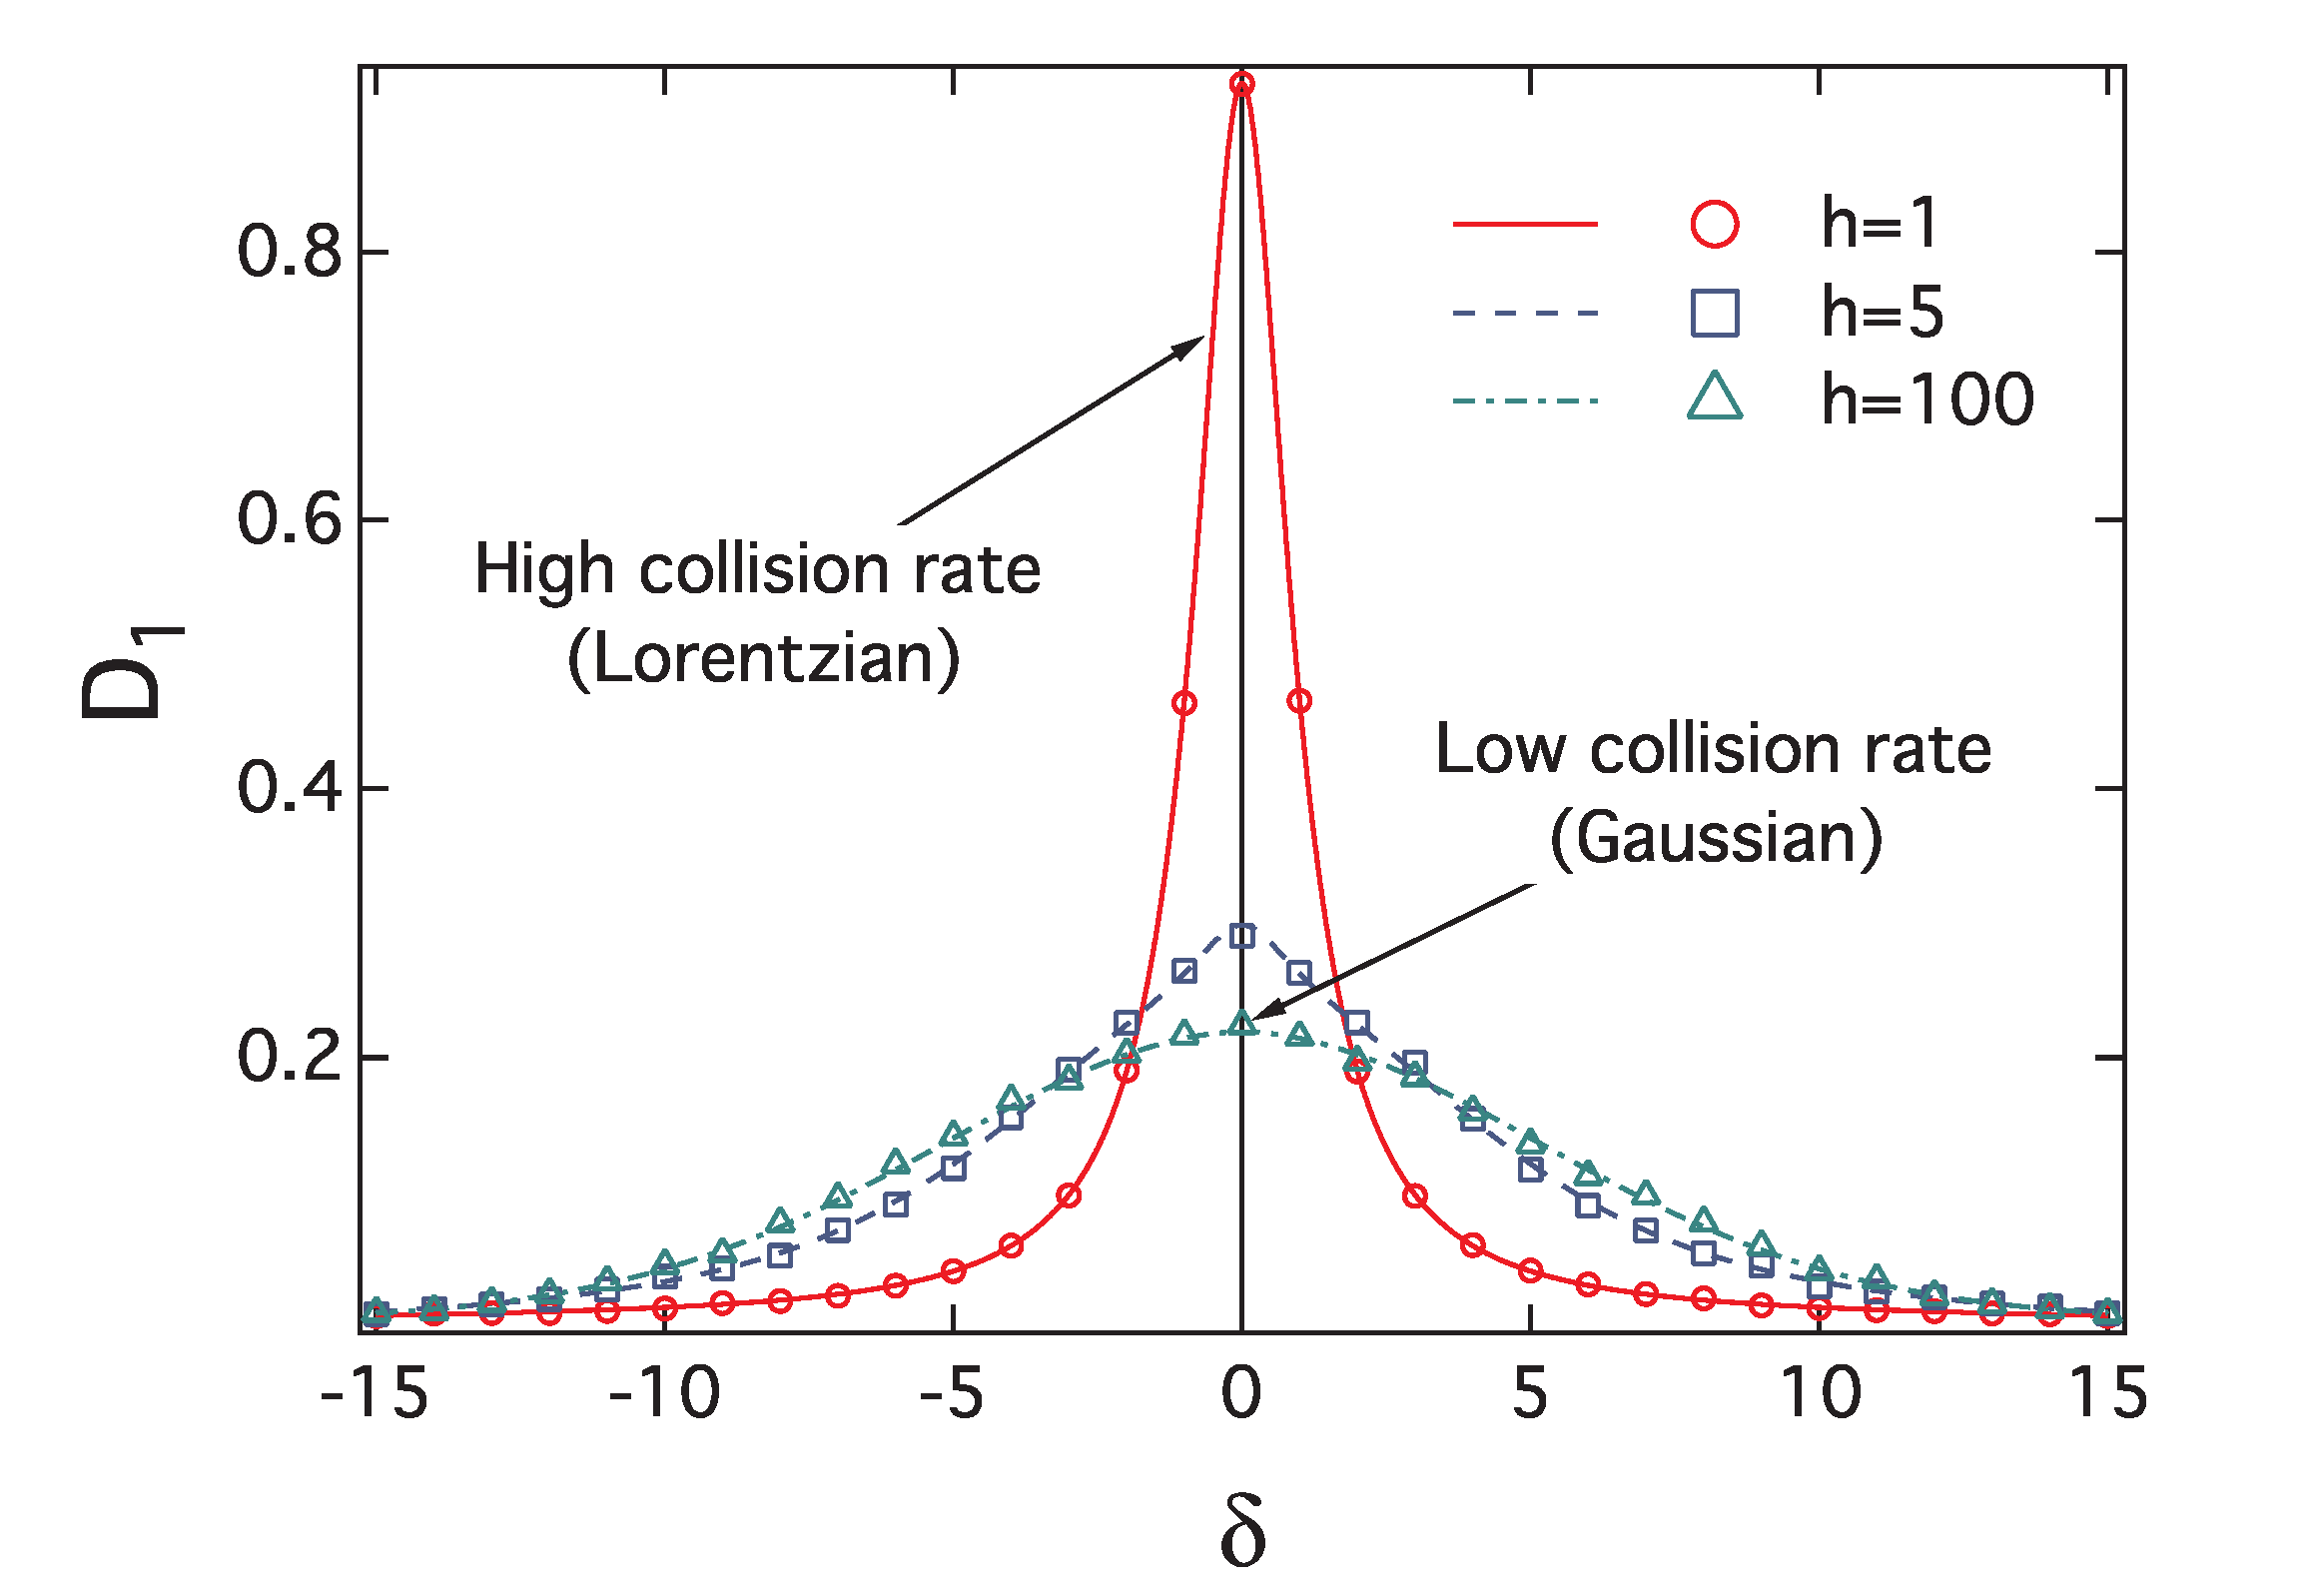
\includegraphics[width=\textwidth]{single_atom.pdf}
\end{center}
\caption{Optical depth $D_1$ versus detuning $\delta$ of a single-atom ensemble with thickness $h=100, 5$ and $1$. The rms axial speed of the atom is $v=5$ for all. Gaussian and Lorentzian profiles are observed when $h=100$ and $h=1$ respectively. When $h=5$, a bulge in the center distorted the curve, making the profile an intermediate state between Gaussian and Lorentzian. Simulations precisely agree with analytical calculations.}
\label{SINGLESPECTRUM}
\end{figure}

The three curves in  Fig.~\eq{SINGLESPECTRUM} also reveal an important phenomenon. As we keep the rms speed of the atom constant and vary the thickness $h$ from extremely big to very small, the spectrum profile undergoes a transition from a broad Gaussian lineshape to a narrow Lorentzian, which is roughly of the natural linewidth.  This narrowing mechanism is consistent with Dicke narrowing. That is to say,  a shorter distance between the two bases, hence a shorter mean free path of the atom, would narrow the spectrum.

\subsection{A Simplified Multiple-Atom Gas}

We can make one more step forward to a simplified model of a gas of $N$ atoms.

In this model, the atom radius is infinitesimal hence there is no atom-atom collision. Moreover, the dipole-dipole interaction between atoms is also neglected. Each atom under these conditions would evolve absolutely independent of others, therefore the dipole moment of each atom at equilibrium is still given by Eq.~\eq{BACKFORTH}. 

If we have $\{v_n\}$ $(n=1,2,3,\cdots,N)$ as the speeds of the $N$ atoms, the total transmission coefficient can be written as:
\bea
\tau_N=1+\sum_{n=1}^{N}\frac{2ie^{-iz_n(t)}d(h,\delta,v_n,t)}{R^2E_0},
\eea
where $z_n(t)$ is the ever-changing position of the $n$th atom. 

Like before, we assume $R\gg 1$, so the approximation in Eq.~\eq{APPROX} is still valid and the total optical thickness of the gas
\bea
D_N(h,\{v_n\}, \delta,t)&\approx&-\frac{4}{R^2E_0}\mathfrak{R}\left[\sum_{n=1}^{N}ie^{-iz_n(t)}d(h,\delta,v_n,t)\right]=\sum_{n=1}^{N}D_1(h,v_n,\delta,t)
\eea

Note that the sum and the time integral in Eq.~\eq{THEORYD} are interchangeable, so the time average is
\bea
\bar{D}_N(h,\{v_n\},\delta)=\sum_{n=1}^{N}\bar{D}_1(h,v_n,\delta)
\eea

Finally, if $\{v_n\}$ obeys Gaussian distribution with rms velocity $u$, the absorption spectrum of the N-atom gas is then
\bea
D_N(h,u,\delta)=ND_1(h,u,\delta)
\eea

We can see that except for a multiplying factor $N$, the spectrum of such a simplified model of gas is essentially identical to the one of a single atom, as in Fig.~\eq{SINGLESPECTRUM}. 
 
This is the end point of the analytical calculations. 

If we want to investigate the influence on the spectrum brought by atom-atom collisions, we have to turn to simulations.

More details about our simulations will be introduced in next section. Here, as a premiere, we present the simulation results for a gas of N atoms with and without atom-atom collisions in Fig.~\eq{COLLISION} (dipole-dipole interaction is still not considered in either case). It is clear that as we adopt a big atom radius so that atom-atom collisions become very frequent, the lineshape is significantly narrowed. 

\begin{figure}[h!]
\begin{center}
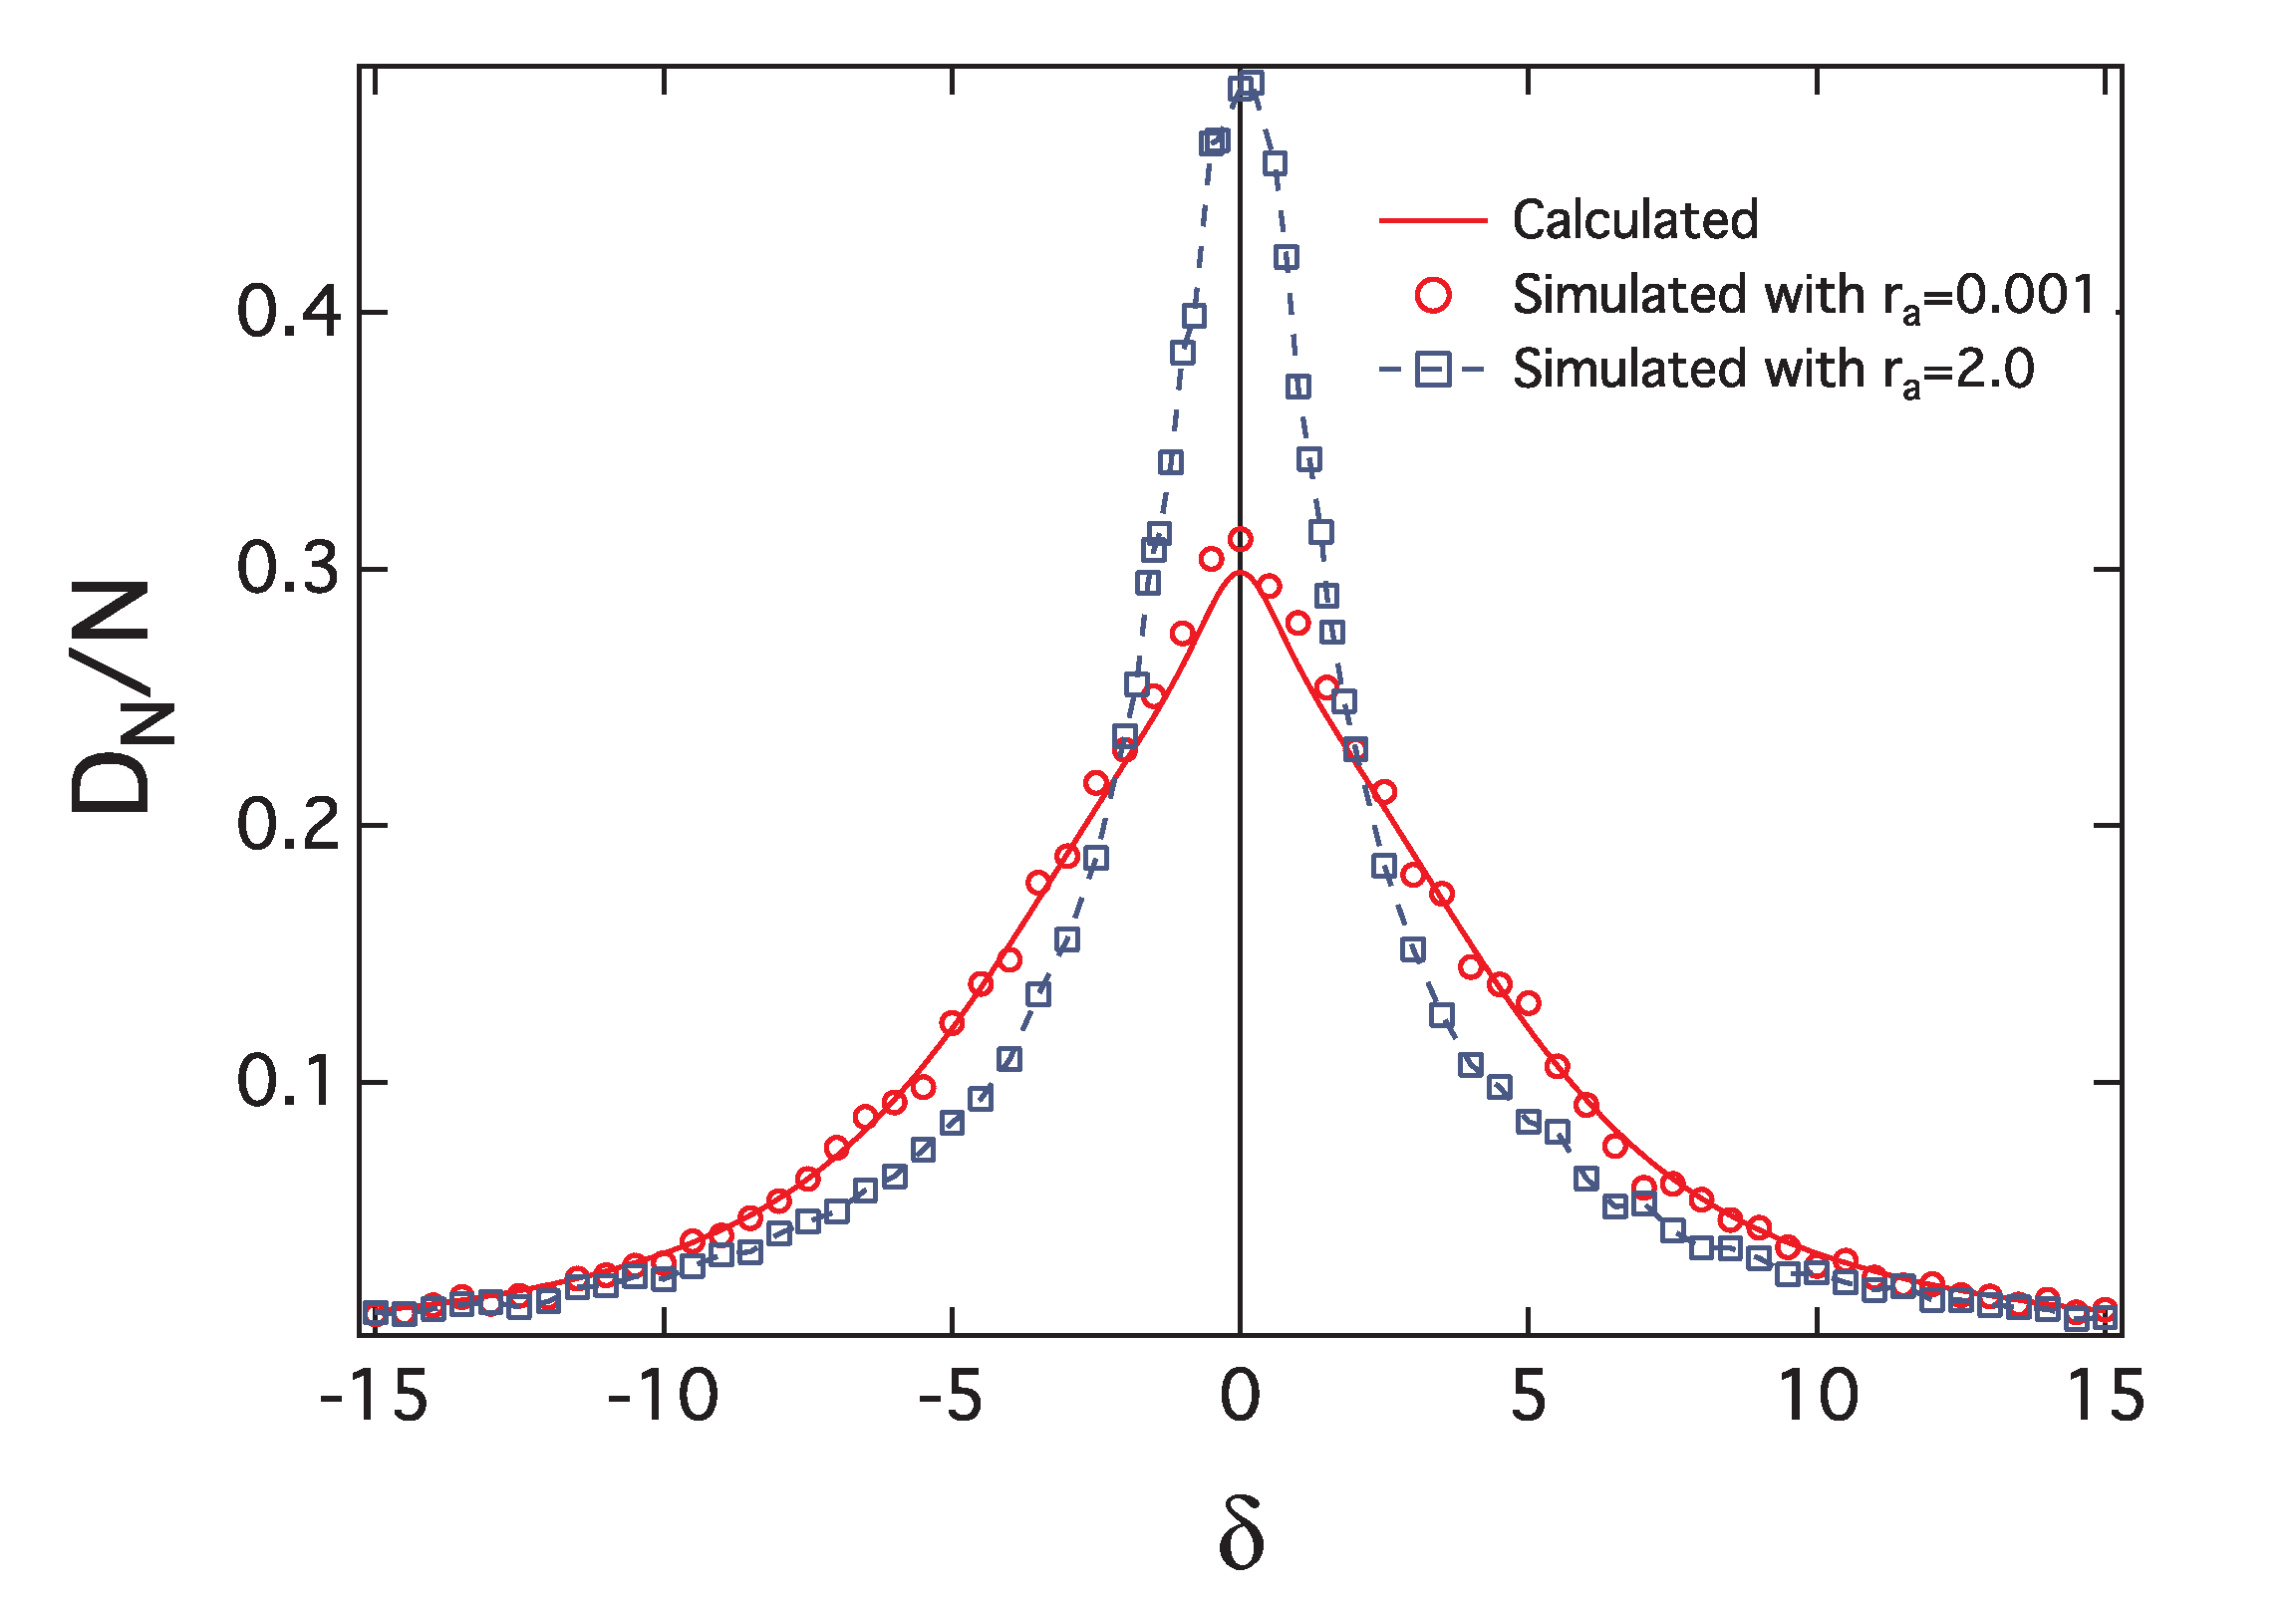
\includegraphics[width=\textwidth]{COLLISION.pdf}
\end{center}
\caption{$D_N/N$ versus $\delta$ with different atom-atom collision ratios. The solid line is calculated by Eq.~\eq{ONEATOMSPECTRUM}, identical to $D_1$ of $h=5$ in Fig.~\eq{SINGLESPECTRUM}. The black crosses correspond to a simulation where atom radius $r_a=0.001$ and the program recorded exactly zero atom-atom collisions. While the red dots correspond to a simulation where $r_s=2.0$ so about half of the collisions are mutual collisions between atoms. In all cases, $N=10$, $u=5$, $R=\sqrt{256/\pi}$ and $h=5+2r_a$. Note that the thickness of the disk has been adjusted to remove any effective shortening of the disk due to the assumption that each atom is a rigid sphere of radius $r_a$.}
\label{COLLISION}
\end{figure}
In summary, if dipole-dipole interactions between atoms are completely absent, either by squeezing the disk in the $z$-direction or by increasing the atom radius, we would end up with a narrower lineshape in the absorption spectrum. Essentially, these two approaches are doing the same thing: reducing the mean free path of the atoms.

\section{Simulations of Multiple-atom Gases}

\subsection{Procedure and Validity of the Simulation Program}

Most of our effort is put into the simulations including dipole-dipole interaction. First of all, some details about our simulations will be introduced. 

\subsubsection{The Initial State of the Evolution}

We assume that, initially, the gas sample is evenly distributed in the circular disk. The atoms obey the Maxwell-Boltzmann velocity distribution and have the same root-mean-squared speed in all three dimensions.

Although the initial states of atoms' dipole moments are irrelevant to the final state as shown in Sec. II, it is still worthwhile to carefully choose the initial states so that the system would relax as soon as possible. This is critical when we deal with a large number of atoms for the time efficiency in computation now becomes a major concern. 

As soon as the incident field is turned on, each atom would be excited by the incident field as well as the dipolar fields from all the other atoms. The time needed to establish the total electric field inside the sample is so short that during which the displacements of the atoms are negligible.  Therefore, we still assume the atoms would stay stationary until the correlations are set up. That means, in our simulations, after the initializations of positions and velocities, the first step is to solve the same hierarchy of equations for the dipole moment of each atom as in a stationary-atom simulation. Just like in the stationary samples, the resonance frequency of each atom has a Doppler shift of $\Delta\omega=kv$. The solutions to these $6N$ linear equations provide the initial states of the dipole evolution described by Eq. ~\eq{DIPOLEEQ}. Essentially, an inhomogeneously broadened static sample in our previous simulations is treated as an initial state in our current simulations. We investigate what would happen when the atoms are moving and colliding.

\subsubsection{Integrating the Evolution Equations and Sampling}

We use adaptive-stepsize Runge-Kutta method to integrate Eq.~\eq{DIPOLEEQ} numerically. The coordinates of the $n$th atom $\mathbf{r}_n$ change with time as the atom moves. Between two successive collisions, the displacement of an atom is simply linear to time. However, this linear dependence would be interrupted by a collision for the velocity always alters its direction in the rigid-sphere model. Consequently, we have to halt the Runge-Kutta integration when a collision happens, update the atom that just collided with the new velocity and then resume the computation.

In the simulations with stationary atoms, we took average over many statistically independent static samples. Now we work on the time average of only one sample instead.  We wait for a time much longer (ten times longer) than the relaxation time of the system, and then begin to take a large number of snapshots of the system's state at times. The time interval between successive snapshots is also longer than the relaxation time to ensure the independence of the samples. Each snapshot works as a sample in our analysis. 


\subsubsection{Collective Lamb Shift: Replicating the Result from Stationary-Atom Simulations}
 
In the simulations of stationary atoms, collective Lamb shifts are observed in dense gases when inhomogeneous broadening is added. For moving atoms,  the CLS is retained as time goes on. This is natural since the model of moving atoms is closer to a real gas.

\begin{figure}[h!]
\begin{center}
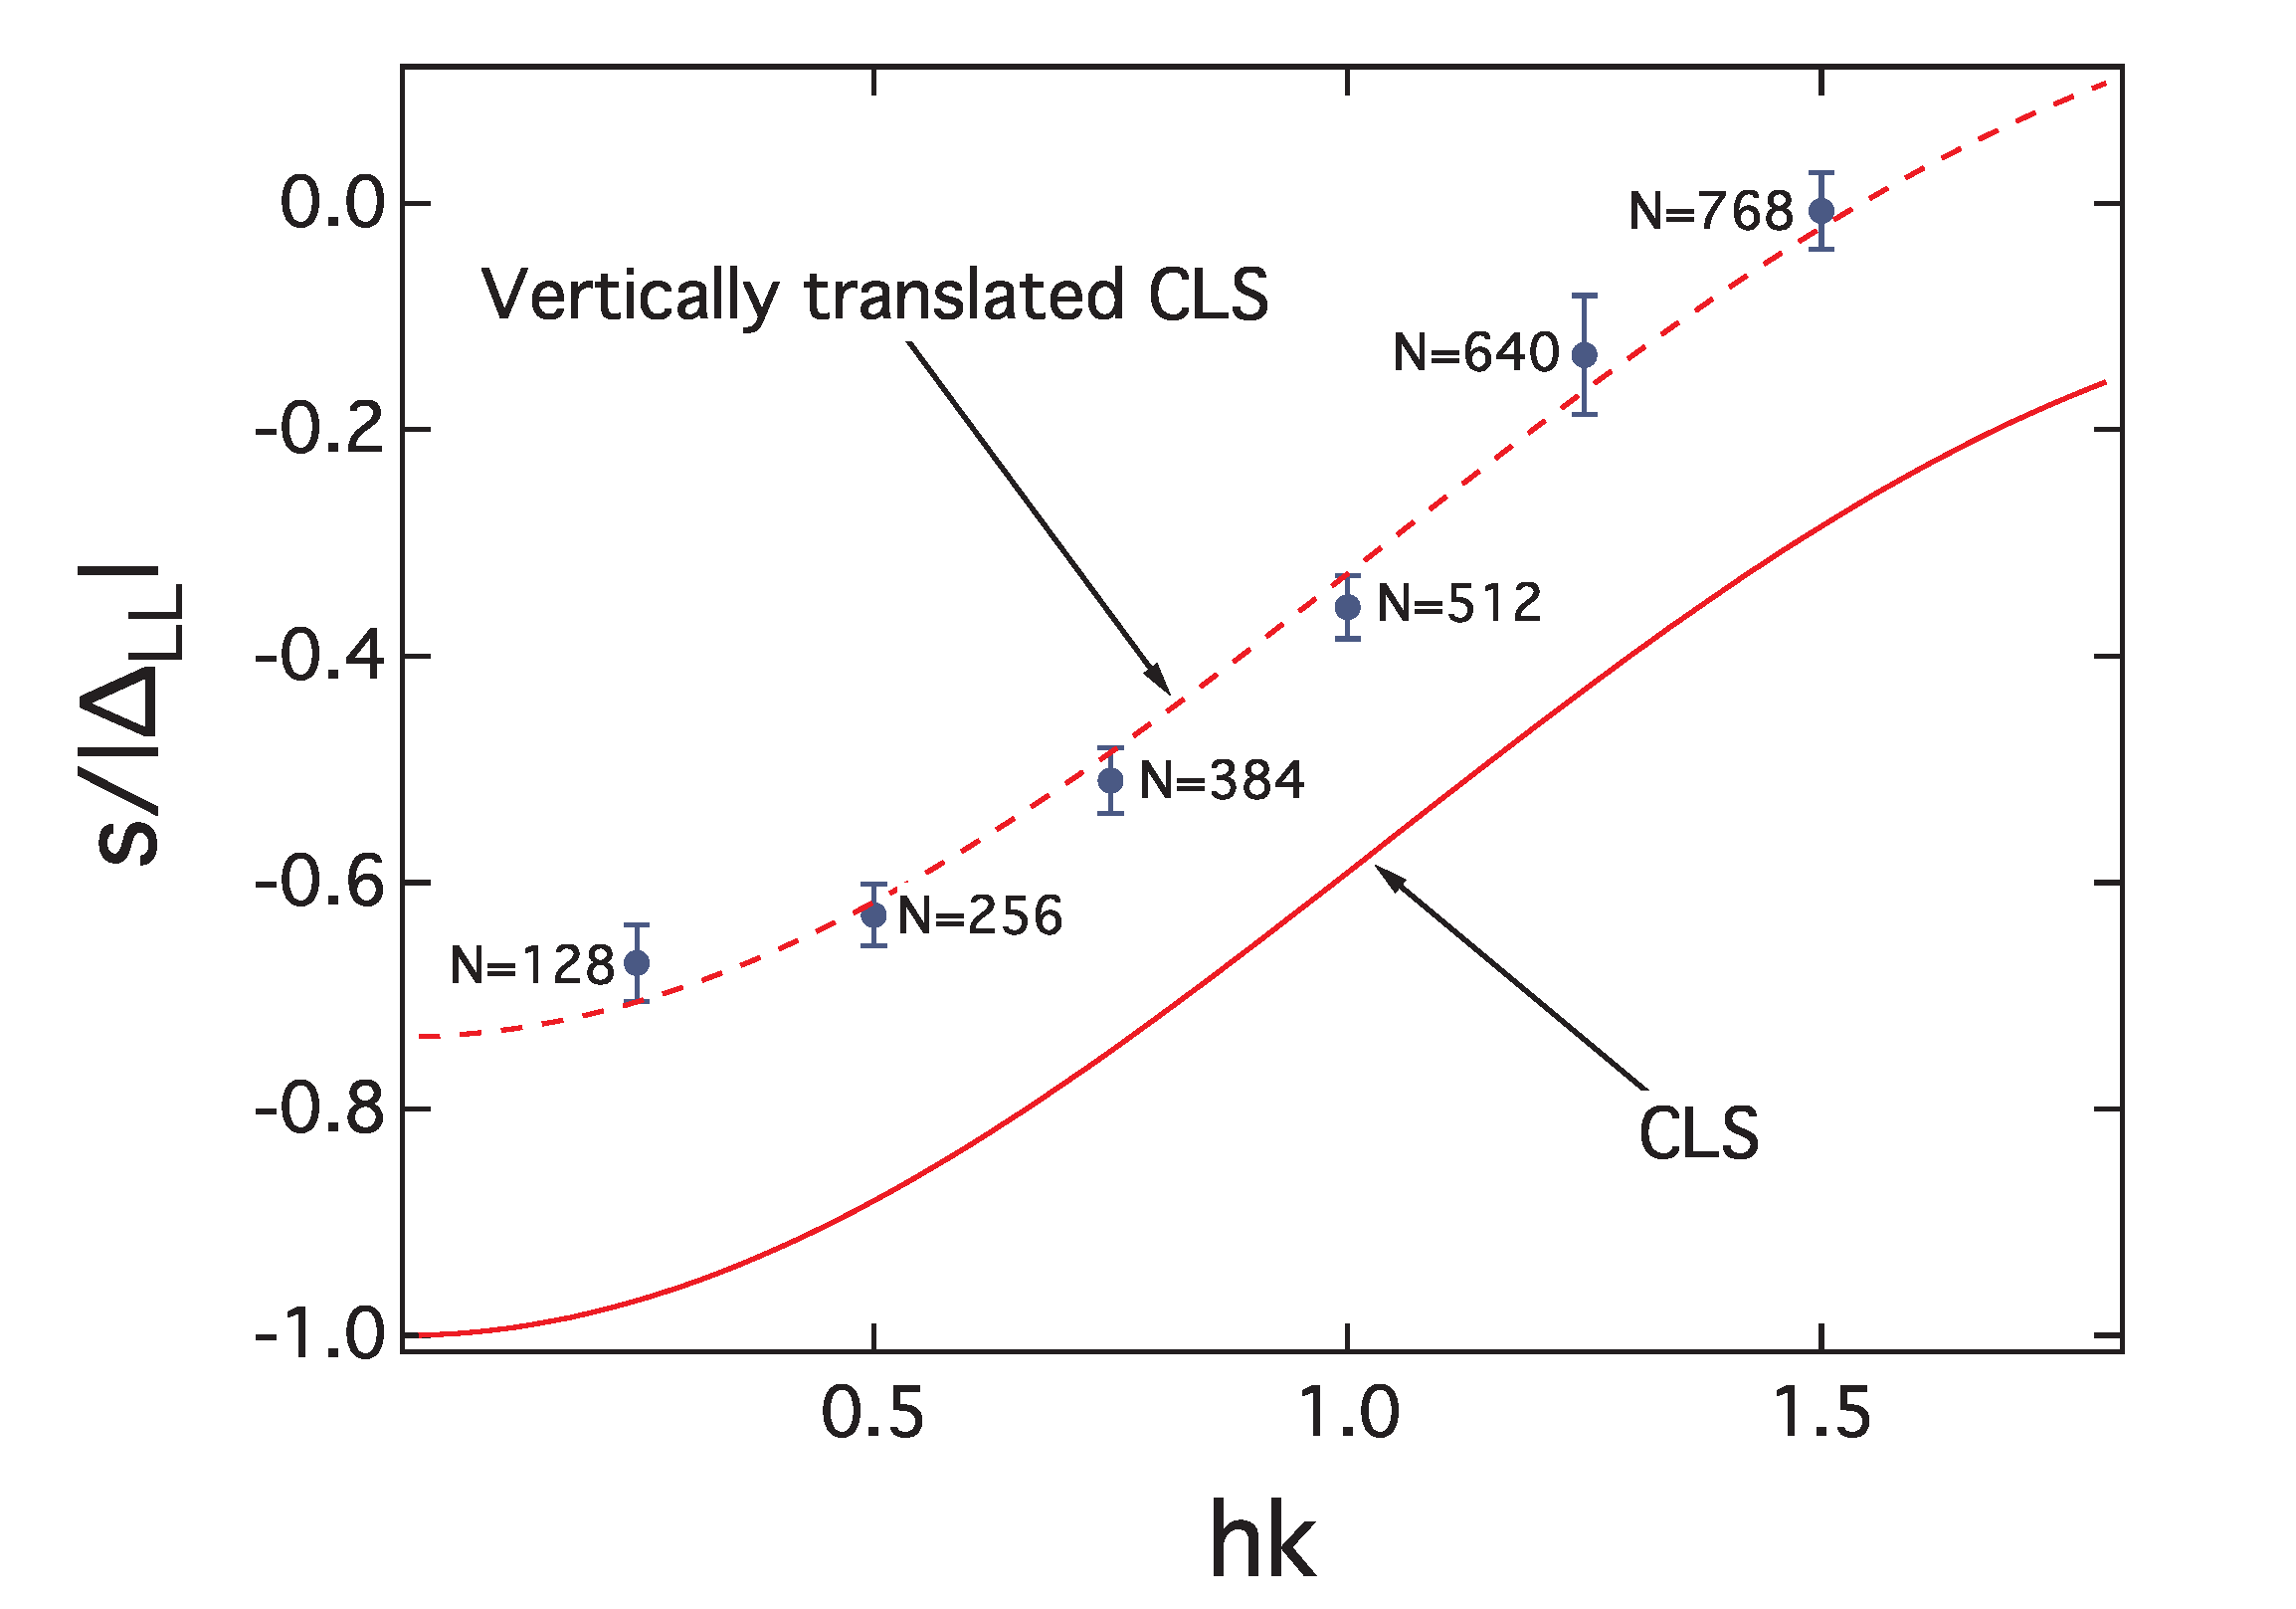
\includegraphics[width=\textwidth]{CLS.pdf}
\end{center}
\caption{The shift of the absorption line $s$ versus the thickness $h$ in a dense gas of moving atoms. $\Delta_{LL}$ is the standard LL shift.}
\label{CLS}
\end{figure}

FIG.~\eq{CLS} shows similar oscillations of the numerical and theoretical CLS. The dashed line is the vertically translated version of the theory. Note that no matter in the experiments ~cite{PhysRevLett.108.173601}, stationary-atom simulations ~cite{PhysRevLett.112.113603} or moving-atom simulations, there is always an additive constant to fit the data points.  The maximum atom number we have tested is $N=768$, for our simulation is restricted by the computing power. This result provides anther proof of the validity of our simulation program.

Similarly to stationary atoms, when the disk is very thin ($hk=0.25$ and $N=128$ in this case), the numerical result deviates from the curve because two dimensional behavior becomes important at this thickness.

\subsection{Broadening of the Dicke-narrowed lineshape in a Dense Gas}

By varying the density of the gas, we found new signs of coorporative effects in the absorption spectra.

\begin{figure}[h!]
\begin{center}
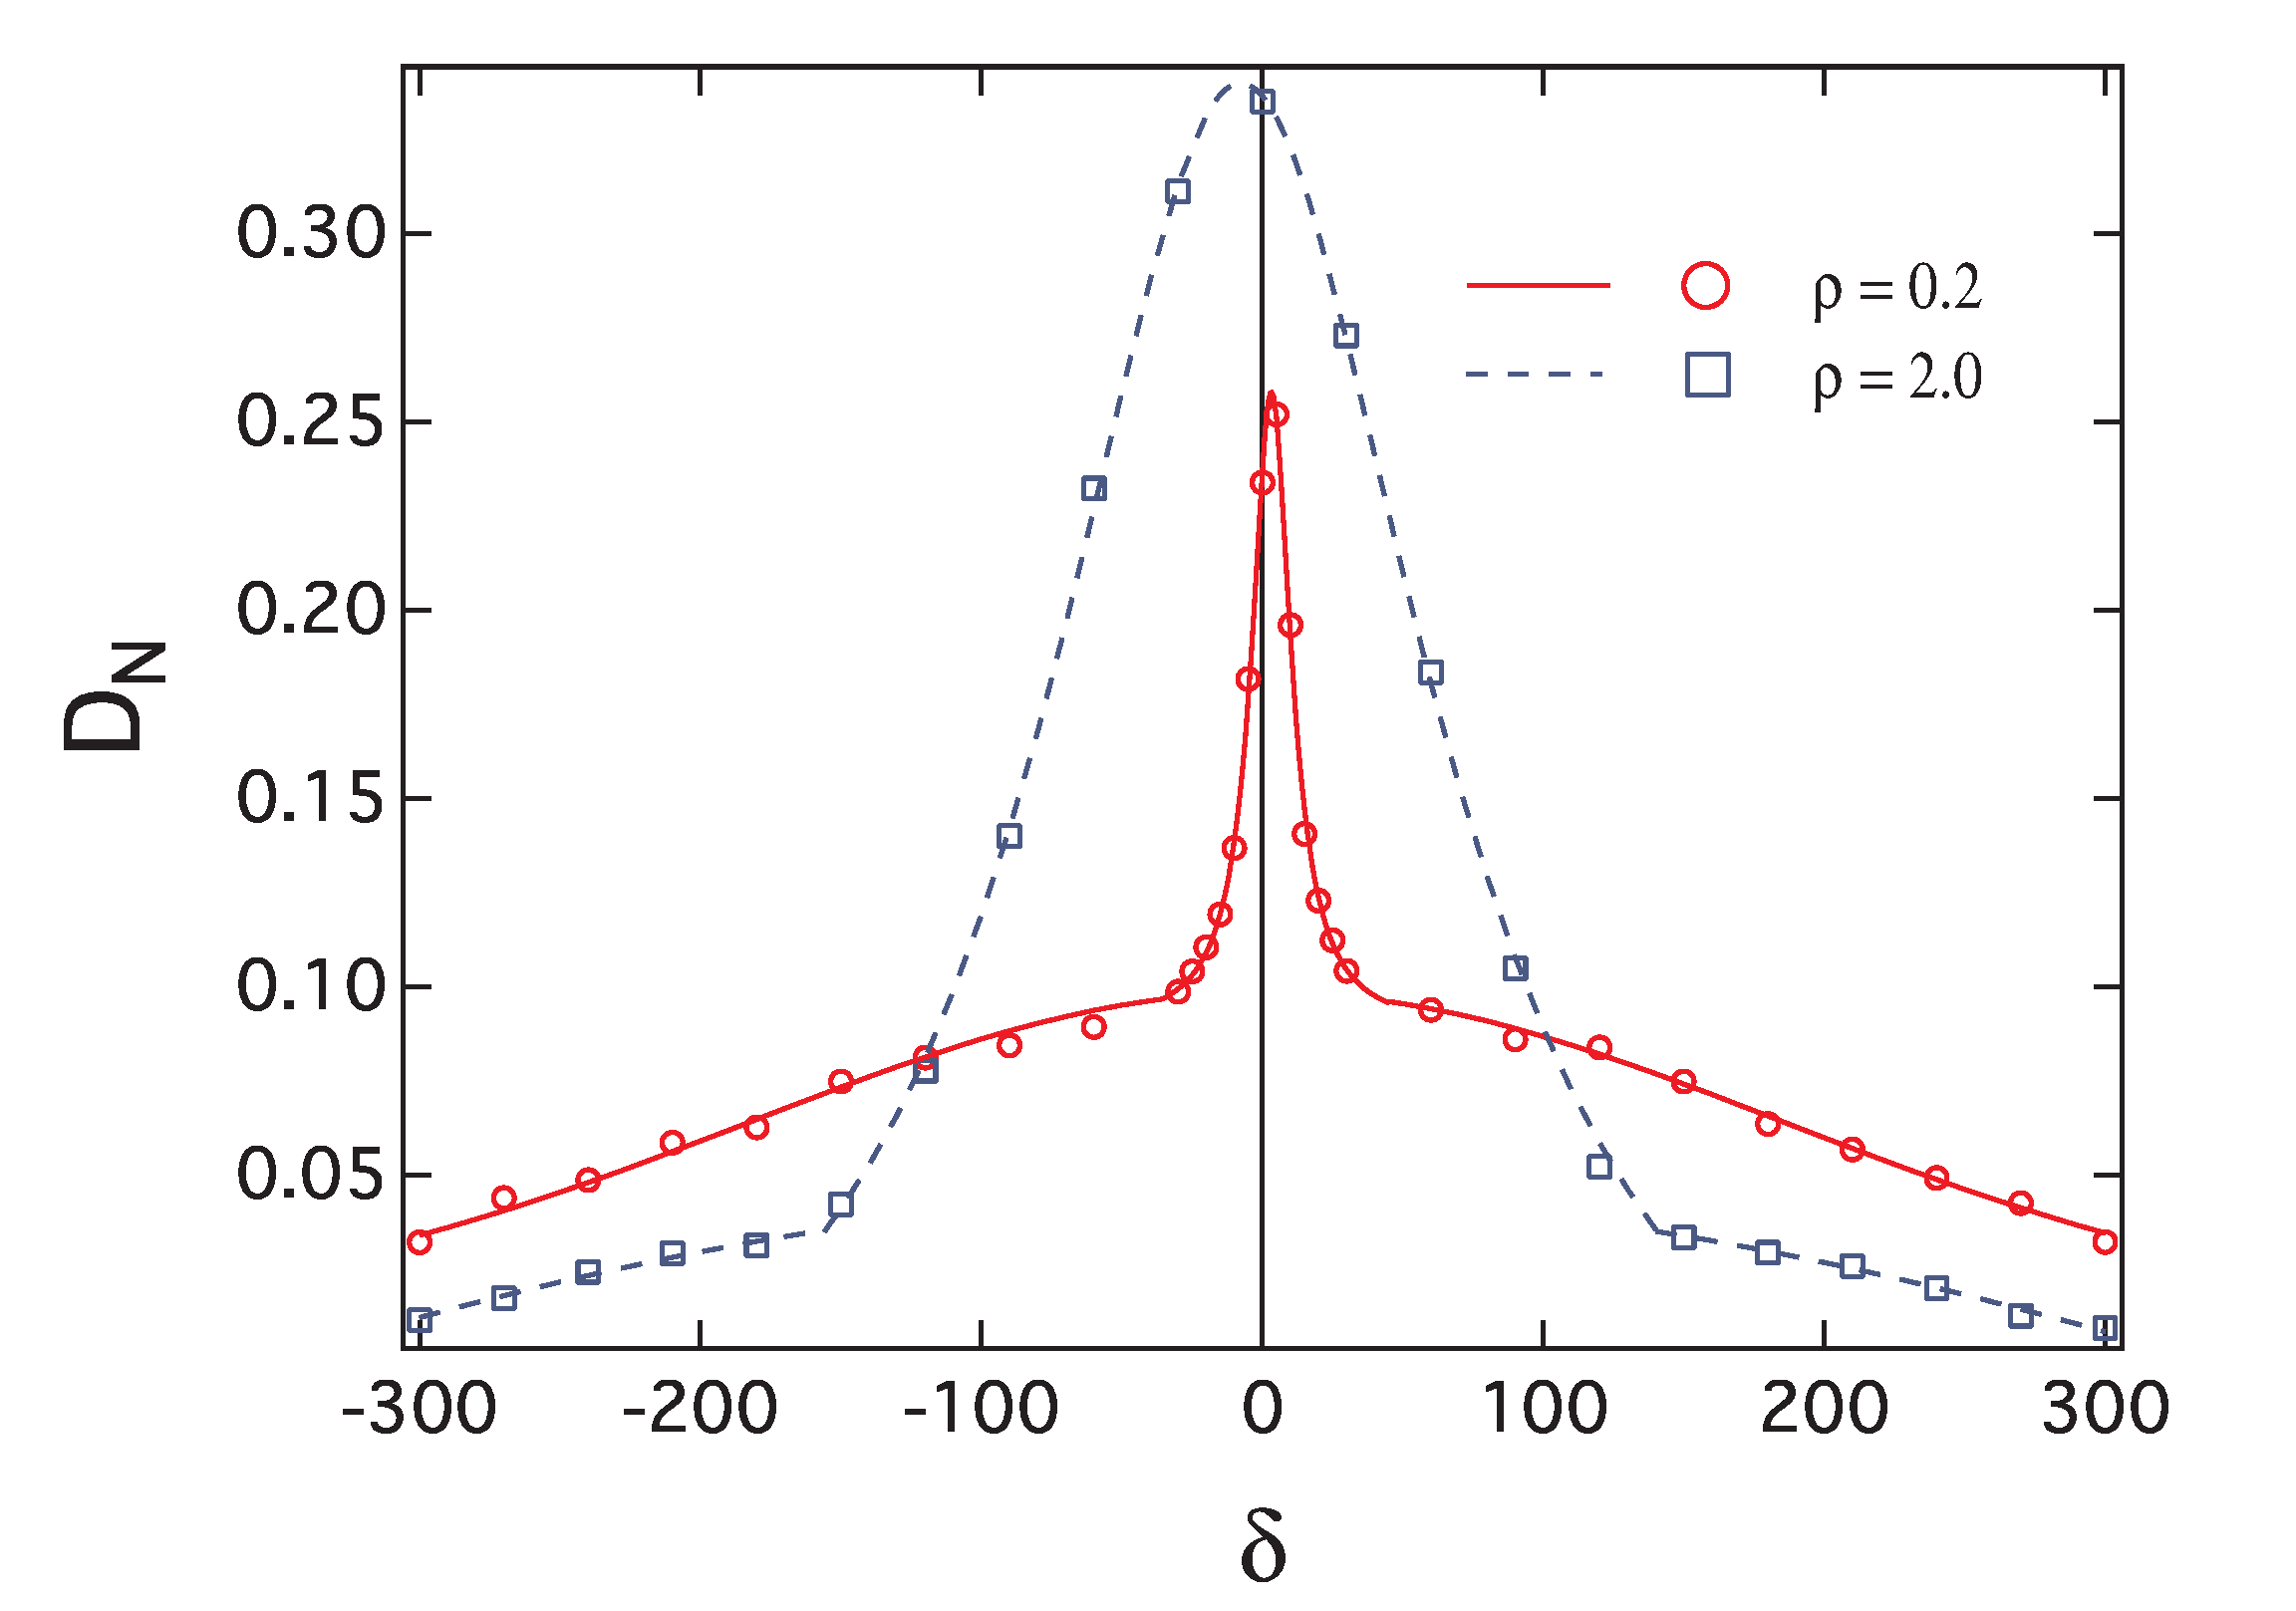
\includegraphics[width=\textwidth]{DICKE.pdf}
\end{center}
\caption{Optical thickness $D_N$ versus $\delta$ in two samples with different densities but the same number of atoms $N=256$. The thickness of the disk $h=5$ (red) and $0.5$ (blue) respectively. In both cases, the rms velocity of atoms $u=5$ and $R=\sqrt{256/\pi}$. The radius of an atom is $r_a=0.01$, so atom-atom collisions are very rare.}
\label{DICKE}
\end{figure}

As shown in FIG.~\eq{DICKE},  in a dilute gas ($\rho k^3=0.2$), based on a Gaussian profile from inhomogenous broadening, a very sharp Lorentzian peak arises near resonance. This is a typical phenomenon of Dicke narrowing. Note that in Sec. II, we also have a narrowing effect on the lineshape from collisions, nevertheless, what we observed there is more like a continuous transition from Gaussian to Lorentzian, not an abrupt Lorentzian peak right over a Gaussian base. So we may conclude here that in a classical gas, the typical appearance of a Dicke narrowed spectrum does not merely result from collision. In order to produce such a lineshape, dipole-dipole interactions (i.e. cooperative effects) must be present.

In the high density regime ($\rho k^3=2$) , the spectrum is still composed of two parts: Gaussian in the side wings and Lorentzian in the center. However, the central peak, as a signature of Dicke narrowing, is remarkably broadened, although the collision rate is much higher.

\begin{figure}[h!]
\begin{center}
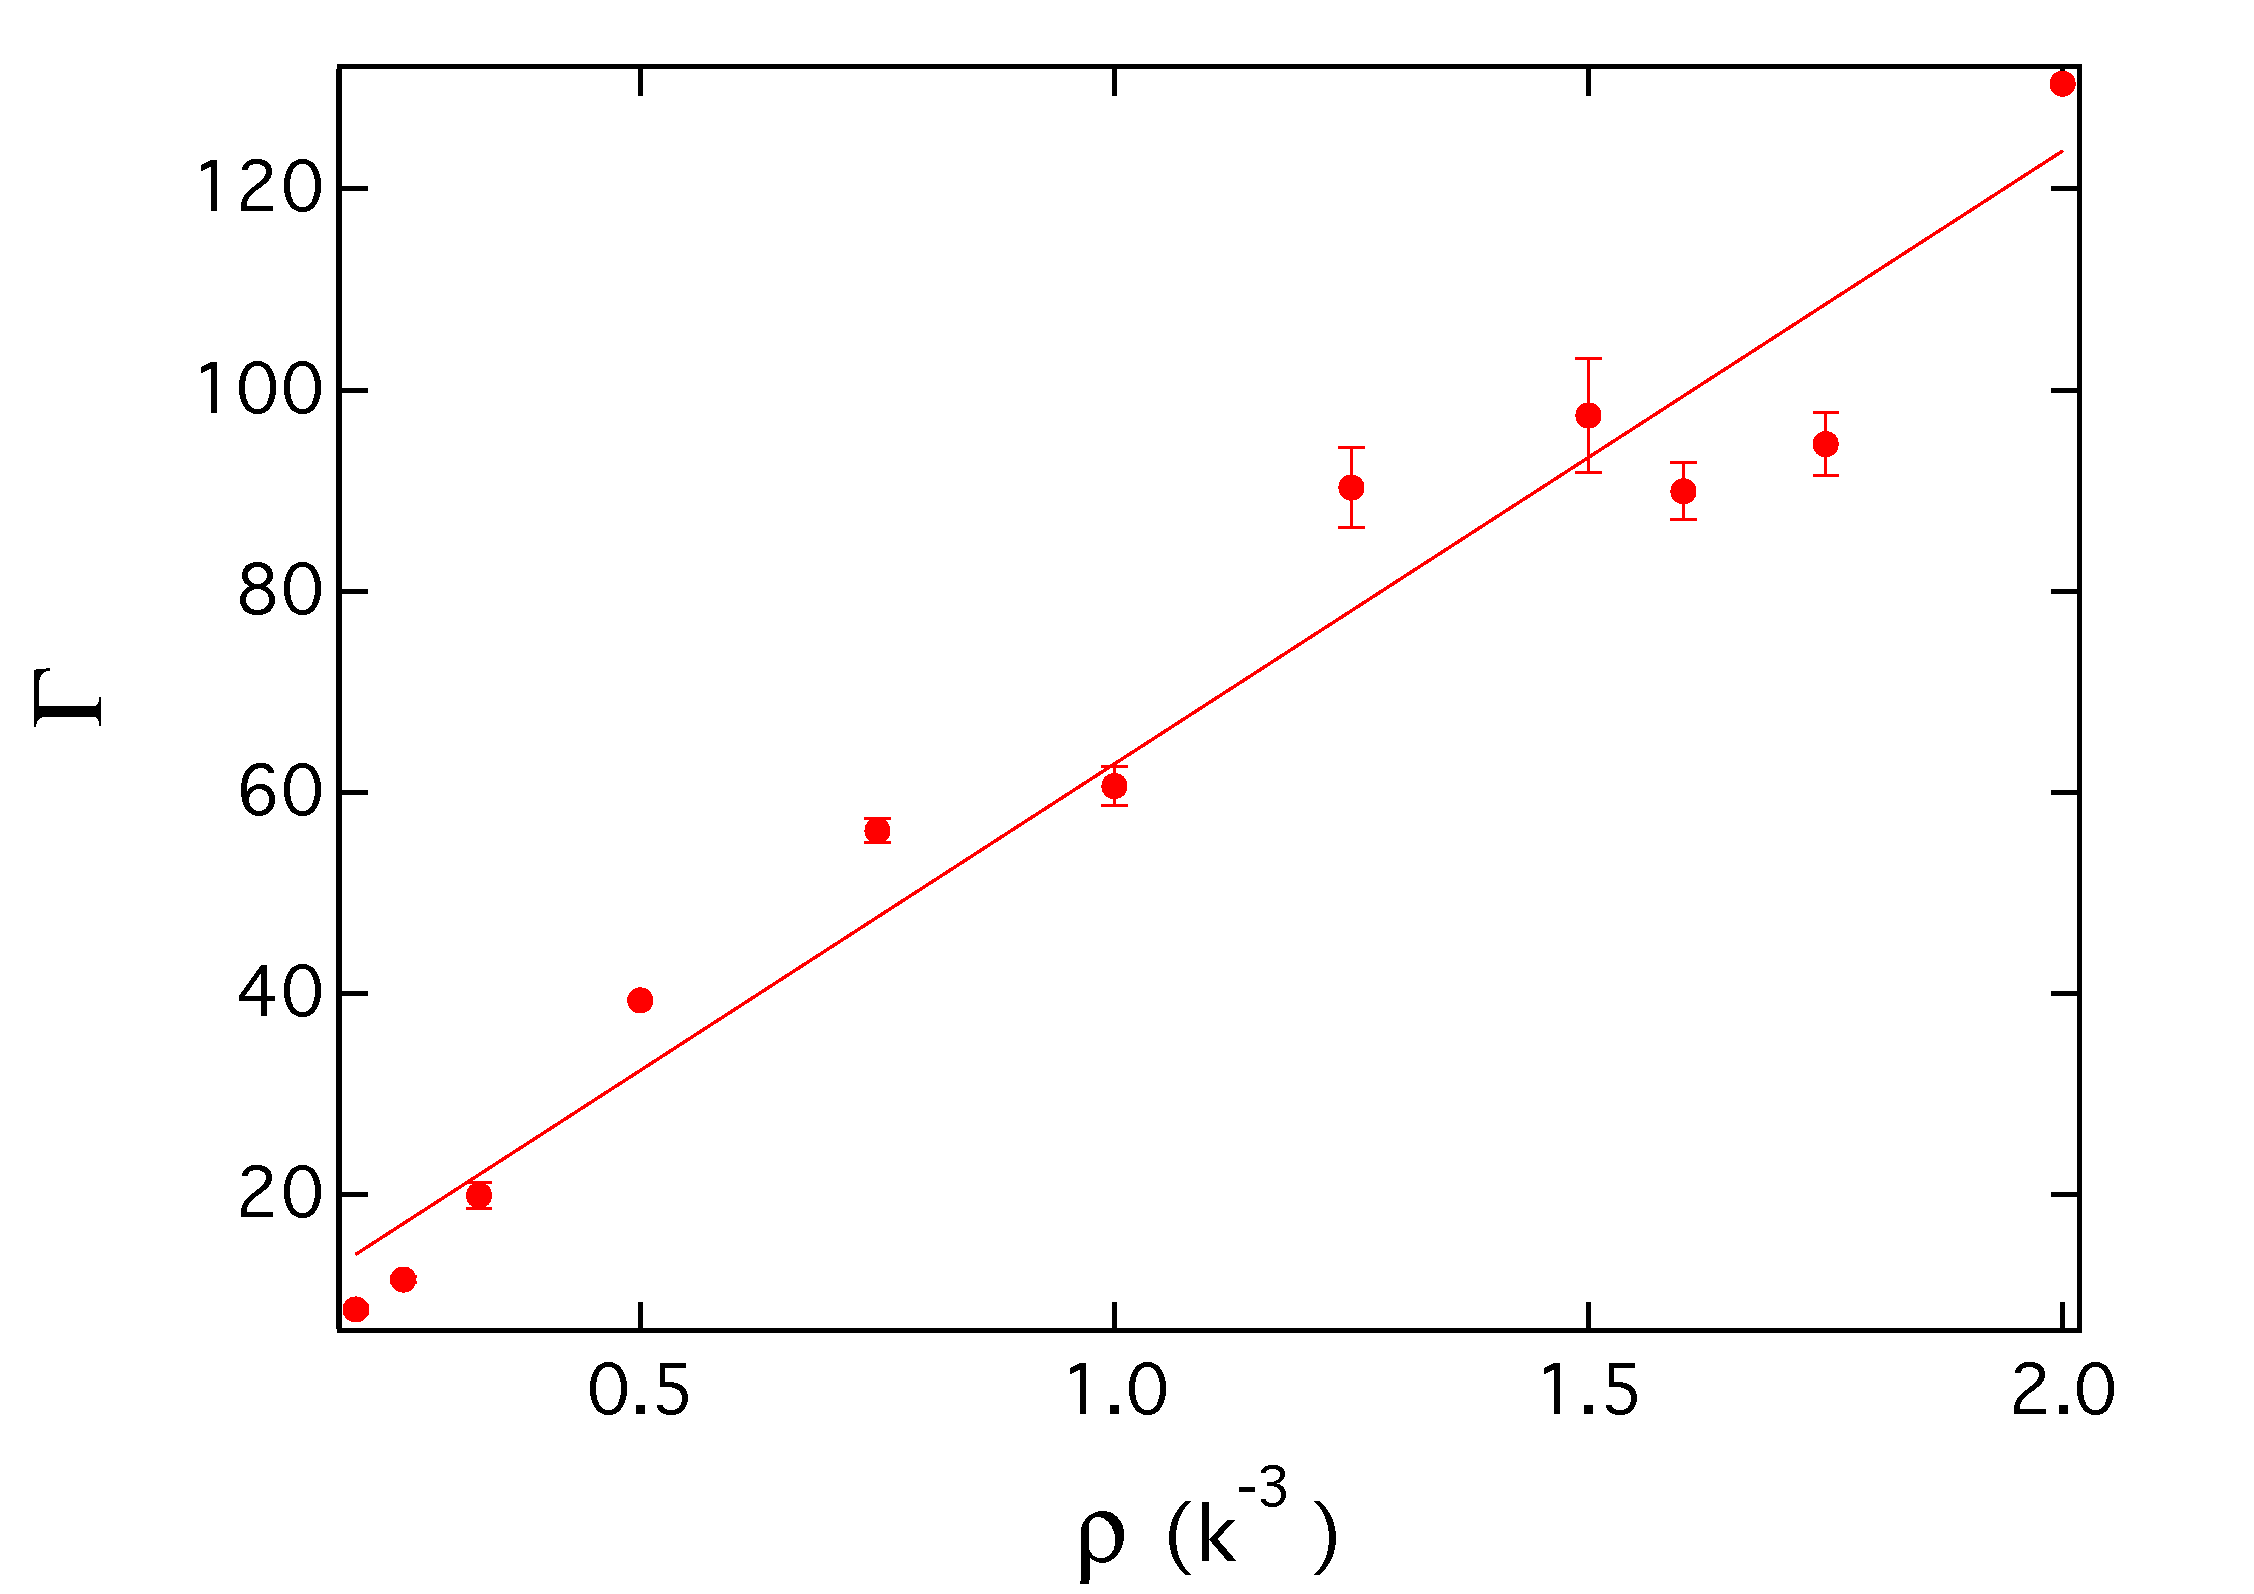
\includegraphics[width=\textwidth]{FWHM.pdf}
\end{center}
\caption{FWHM of the Lorentzian peak vs. density for same number of atoms $N=256$. The density is changed by varying the thickness of the disk.}
\label{FWHM}
\end{figure}

Recall the results we obtained in Sec. II, without dipole-dipole interactions, a higher frequency of either atom-wall collisions or atom-atom collisions would always narrow the lineshape. Conversely, when dipole-dipole interactions kick in, as shown in FIG.~\eq{FWHM}, the width of the Lorentzian peak in the spectrum keeps increasing as the density goes up. 

This broadening shows difference from a conventional Dicke narrowing phenomenon. It can by no means be classified as a collisional broadening, because the rigid sphere model is used all through our simulations thus the internal state of the atom is not considered at all. Since all of our work is done classically,  comparing to the results in Sec. II, we conclude that this broadening is a cooperative effect because of the light re-scattering processes between atoms.

\chapter{Conclusion}
For stationary atoms, an analytical calculation of radiated fields is feasible in simple cases such as a single atom, two atoms, and a non-cooperative Gaussian sample. We derived explicit expressions of total radiation power in these cases. The discrepancy between a continuous medium and a sample of discrete non-interacting atoms touches some fundamental problems in the traditional optics which is essentially a mean-field theory. More details are discussed in other works.

We carried out simulations for stationary atoms with dipole-dipole interactions. A direct comparison of the total radiated power with independent atoms has revealed the cooperative effects.

In the second part of this paper, we incorporated atomic motion, including collisions, in our classical-electrodynamics simulations of light propagation in a dense gas sample. The introduction of atomic motion not only reproduces the same results as we achieved on stationary atoms, such as collective Lamb shift, but also demonstrates new spectral features that result from cooperative effects on the optical response of the gas.

Starting from Eq.~\eq{DIPOLEEQ}, our calculations and simulations on moving atoms confirms that for a gas confined in a certain container like a circular disk that we adopted, if each atom is supposed to be polarized solely by the incident light but electromagnetically independent of any other atoms, a shorter mean free path would narrow the absorption spectrum. This is consistent with the conventional theory of Dick narrowing.

However, a confirmative signature of Dick narrowing, i.e., a sharp Lorentzian peak over a wide Gaussian base, would manifest only when dipole-dipole interactions are included in the simulations. Even more interesting, the cooperative response in this system reverses the dependence of the line width on the gas density. An extra broadening is observed based on a Dick-narrowed spectrum. ~\cite{Sci.325.1510}.





\bibliography{bib_summary}



% appendices: we put them after the references in what ever order
% we prefer
%\input{appendices/dsmethod.tex}
\end{document}

